\documentclass[a4paper]{scrartcl}

\usepackage[
	fancytheorems,
	fancyproofs,
	noindent
]{adam}

\usepackage{tikz}
\usepackage{subcaption}
\usetikzlibrary{calc,angles,quotes,decorations.pathreplacing}

\tikzset{every picture/.style={line width=0.5pt}}

\newcommand{\rank}{\operatorname{rank}}
\newcommand{\nullity}{\operatorname{null}}
\newcommand{\adj}{\operatorname{adj}}
\newcommand{\diag}{\operatorname{diag}}

% The aside environment uses \subsection* internally, which (with KOMA)
% resets the subsubsection counter -- save and restore it around asides.
\newcounter{asidesubsubsave}
\AtBeginEnvironment{aside}{\setcounter{asidesubsubsave}{\value{subsubsection}}}
\AtEndEnvironment{aside}{\setcounter{subsubsection}{\value{asidesubsubsave}}}

\title{Vectors and Matrices}
\author{Adam Kelly (\texttt{ak2316@cam.ac.uk})}
\date{\today}

\allowdisplaybreaks

\begin{document}

\maketitle

Vectors and Matrices covers topics in both algebra and geometry, and the ways in which they relate to one another. Starting from the complex numbers, we will work our way up through vectors in three dimensions, vectors in general, and then to linear maps and the matrices that represent them -- along the way meeting determinants, eigenvalues, and the various canonical forms a matrix can be put into. The approaches used throughout are quite varied in their nature (they can be abstract or concrete, conceptual or computational, and so on), and being able to switch fluently between these viewpoints is one of the main skills this course develops.

This article constitutes my notes for the `Vectors and Matrices' course, held in Michaelmas 2020 at Cambridge. These notes are \emph{not a transcription of the lectures}, and differ significantly in quite a few areas. Still, all lectured material should be covered.

\tableofcontents



\section{Complex Numbers}

The complex numbers arose through the study of polynomials, but there is hardly an area of modern mathematics where they are not of use, with applications stretching from number theory to geometry to quantum mechanics.


\subsection{Defining the Complex Numbers}

We are going to start right at the beginning, though some familiarity with complex numbers is assumed.
We will construct the set of complex numbers, denoted by $\C$, from the real numbers $\R$ by adjoining an element $i$ with the property that $i^2 = -1$.

\begin{definition}[Complex Numbers]
	A \vocab{complex number} is a number $z \in \C$ of the form $z = x + yi$ with $x, y \in \R$ such that $i^2 = -1$. 
	
	We call $x = \re(z)$ the \vocab{real part}, and $y = \im(z)$ the \vocab{imaginary part} of $z$.
\end{definition}

The reals are a subset of the complex numbers, as for $x \in \R$, we have $x + 0i \in \C$. 

\subsubsection{Basic Operations}

With the complex numbers defined, we have to come up with some things to do with them.
We can add, subtract, multiply and divide complex numbers in a sensible way, and indeed they form a \emph{field} (we will elaborate on this later).

\begin{definition}[Basic Operations in $\C$]
	Let $z_1 = x_1 + y_1 i$ and $z_2 = x_2 + y_2 i$ be two complex numbers. Then we define \vocab{addition} and \vocab{multiplication} as
	\begin{align*}
		z_1 + z_2 &= (x_1 + x_2) + (y_1 + y_2)i,\\
		z_1 \times z_2 &= (x_1 x_2 - y_1 y_2) + (x_1 y_2 + x_2 y_1)i.
	\end{align*}
\end{definition}

We can see from this definition that the operation of multiplication respects our original requirement that $i^2 = -1$. From these definitions we can also immediately define \vocab{subtraction} and \vocab{division} as the inverse operations of these, with
\begin{align*}
	z_1 - z_2 &= (x_1 - x_2) + (y_1 - y_2)i \\
	\frac{z_1}{z_2} &= \frac{x_1 + y_1 i}{x_2 + y_2 i} \cdot \frac{x_2 - y_2i}{x_2 - y_2 i} = \left(\frac{x_1y_1 + x_2 y_2}{x_2^2 + y_2^2}\right) + \left(\frac{x_2y_1 - x_1 y_2}{x_2^2 + y_2^2}\right)i.
\end{align*}

From the definitions of addition and multiplication, it is clear that both operations are commutative and associative. Indeed, as we also have inverse operations, the complex numbers form groups.

\begin{proposition}[$\C$ is a Group]
	$\C$ with the operation $+$ is an abelian group with identity $0$, and $\C \backslash \{0\}$ with the operation $\times$ is an abelian group with identity $1$.
\end{proposition}
\begin{proof}[Proof Sketch]
	Check definitions and verify that $+$ and $\times$ are indeed associative.
\end{proof}

Another useful operation is the \emph{complex conjugate}. 

\begin{definition}[Complex Conjugation]
  For a complex number $z = x + iy$, we define its \vocab{complex conjugate} to be $\overline{z} = z^* = x - iy$.
\end{definition}

Complex conjugation allows us to extract the real and imaginary parts of a complex number, with
$$
\re(z) = \frac{z+ \overline{z}}{2}, \quad \text{and} \quad \im(z) = \frac{z - \overline{z}}{2i}.
$$
For complex numbers $z_1$ and $z_2$, we have $\overline{(\overline{z})} = z$, $\overline{z_1 + z_2} = \overline{z_1} + \overline{z_2}$ and $\overline{z_1 z_2} = \overline{z_1} \cdot  \overline{z_2}$.

\begin{aside}{Aside: The History of Complex Numbers}

The complex numbers arose through the study of polynomials, and their serious study really began in the study of the \emph{cubic} polynomials of the form\footnote{This form of a cubic equation is a `depressed', and any general cubic can be expressed in this form.}
$$
x^3 - 3px - 2q = 0.
$$
The sixteenth century mathematicians del Ferro, Tartaglia and Cardano discovered that this equation could be solved explicitly, with the result being published in Cardano's 1545 work \emph{Ars Magna} (where he mentioned del Ferro as a first author, and noted that Tartaglia had independently found the same result).
The solution they had obtained was
$$
x = \sqrt[3]{q + \sqrt{q^2 - p^3}} + \sqrt[3]{q - \sqrt{q^2 - p^3}}.
$$
For example, for the cubic $x^3 - 12x - 20$ we obtain the solution $x = \sqrt[3]{16} + \sqrt[3]{2}$. 

Some 30 years later, Rafael Bombelli discussed one particular cubic in his work \emph{l'Algebra}. He looked at $x^3 - 15x - 4 = 0$.
One might observe (through mere trial and error) that $x = 4$ is a solution, but using Cardano's formula, we obtain the solution
$$
x = \sqrt[3]{2 + \sqrt{-121}} + \sqrt[3]{2 - \sqrt{-121}}.
$$
Indeed, Bombelli noticed this and gave an explanation for how these two solutions were essentially the same, even with the presence of the rather puzzling term $\sqrt{-121}$.
His explanation essentially began by noting that if we wrote $\sqrt{-121} = 11i$, then we could find that
\begin{align*}
	\sqrt[3]{2 + \sqrt{-121}} &= 2 + ni \\
	\sqrt[3]{2 - \sqrt{-121}} &= 2 - ni,
\end{align*}
and adding would then result in $2 + ni + 2 - ni = 4$, our other solution.

Inherent in this explanation was an expectation that this $i$ would obey many of the same rules of arithmetic that we would expect of, say, a real number. After this work, contributions from mathematicians such as Descartes, Wallis, de Moivre, Euler, Wessel, Argand, Hamilton, Gauss, Cauchy and many others began to build up a rich theory of the complex numbers, later developing the field of complex analysis, all centered on this construction of some $i$ with the property that $i^2 = -1$. 

\end{aside}

Looking again at the solutions to polynomials it turns out that the complex numbers are sufficient to solve \emph{every} polynomial equation. This result is known as the `Fundamental Theorem of Algebra', and was proved in the 18th century. We will use it frequently in this course, but you will have to wait until a later course to see a proof.
\begin{theorem}[Fundamental Theorem of Algebra]
Let $p(z)$ be a polynomial of degree $n \geq 1$ with complex coefficients. Then $p(z) = 0$ has precisely $n$ (not necessarily distinct) complex roots, counted with multiplicity. 
\end{theorem}

\subsubsection{The Argand Diagram}

There is a geometric way to interpret complex numbers and the way that they operate. We can plot a complex number $z = x + yi$ on the \vocab{Argand diagram} or \vocab{complex plane} by associating it with a point $(x, y)$. We call the $x$ axis the `real' axis, and the $y$ axis the `imaginary' axis.

\begin{center}
  \begin{tikzpicture}
    \draw [->] (-1, 0) -- (3.5, 0) node [right] {$\re$};
    \draw [->] (0, -1) -- (0, 2.75) node [above] {$\im$};
	\draw [->] (0, 0) -- (2.5, 1.7) node [anchor=south west] {$x + yi$} node [pos=0.5, above] {$r$} node [pos=0.3, below] {$\theta$};
    \draw [dashed] (0, 1.7) node [left] {$y$} -- (2.5, 1.7) -- (2.5, 0) node [below] {$x$};
  \end{tikzpicture}
\end{center}

From the complex number written $z= x + yi$, we can plot it in rectangular coordinates. However, it can also be useful to plot it using polar coordinates. With this in mind, we introduce some useful 
definitions.

\begin{definition}[Modulus]
	For a complex number $z = x + yi$, we define its \vocab{modulus} to be $r = |z|$ such that $r \geq 0$ and $r^2 = |z|^2 = x^2 + y^2$.
\end{definition}

Indeed, this definition matches the distance from the origin of the Argand diagram to the point $(x, y)$.

\begin{definition}[Argument]
	For a non-zero complex number $z$, we define its \vocab{argument} to be $\theta = \arg(z)$, a real number such that $z = r(\cos \theta + i \sin \theta)$. We say this is the \vocab{polar form} of $z$.
\end{definition}

From this, we get that for $z = x + yi$,
$$
\cos \theta = \frac{x}{\sqrt{x^2 + y^2}}, \quad \sin \theta = \frac{y}{\sqrt{x^2 + y^2}}, \quad \text{and} \quad \tan \theta = \frac{y}{x}.
$$

An important point to note is that $\arg(z)$ is only defined up to multiples of $2 \pi$, as mapping $\theta \mapsto \theta + 2\pi$ leaves $z$ unchanged. So, to make $\theta$ unique (which is often useful), we typically restrict its range. For example, if we restrict $- \pi < \theta \leq \pi$, we get the \vocab{principal value} of $\theta$.

Using the Argand diagram, there is a geometric 
way to define addition, multiplication and complex conjugation. Addition and subtraction correspond to parallelograms constructed as shown.

\begin{center}
	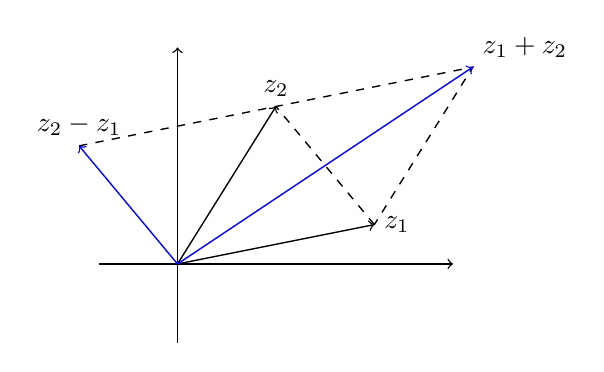
\begin{tikzpicture}
	  \draw [->] (-1, 0) -- (3.5, 0) node [right] {$\re$};
	  \draw [->] (0, -1) -- (0, 2.75) node [above] {$\im$};
	  \draw [->] (0, 0) -- (2.5, 0.5) node [anchor=west] {$z_1$};
	  \draw [->] (0, 0) -- (1.25, 2.0) node [anchor=south]{$z_2$};
	  \draw [dashed] (-1.25, 1.5) -- (3.75, 2.5) node [anchor=south west] {$z_1 + z_2$}  -- (2.5, 0.5);
	  \draw [dashed] (2.5, 0.5) -- (1.25, 2.0);

	  \draw [->, color=blue] (0, 0) -- (3.75, 2.5); 
	  \draw [->, color=blue] (0, 0) -- (-1.25, 1.5) node [color=black, anchor=south] {$z_2 - z_1$};
	\end{tikzpicture}
  \end{center}

  Complex conjugation corresponds to reflection in the real axis.

  \begin{center}
	\begin{tikzpicture}
	  \draw [->] (-1, 0) -- (3.5, 0) node [right] {$\re$};
	  \draw [->] (0, -2) -- (0, 2) node [above] {$\im$};
	  \draw [->] (0, 0) -- (2.5, 1.4) node [anchor=south west] {$z = x + yi$};
	  \draw [color=blue, ->] (0, 0) -- (2.5, -1.4) node [color=black, anchor=south west] {$\overline{z} = x - yi$};
	  \draw [dashed] (2.5, 1.4) -- (2.5, -1.4);
	\end{tikzpicture}
  \end{center}

  Multiplication is slightly more complex. If we have two complex numbers in polar form, $z_1 = r_1 (\cos \theta_1 + i\sin \theta_1)$ and $z_2 = r_2 (\cos \theta_2 + i \sin \theta_2)$, then expanding and applying the angle sum identities gives $z_1 z_2 = r_1 r_2 (\cos (\theta_1 + \theta_2) + i \sin (\theta_1 + \theta_2))$.
  This gives the following.

  \begin{proposition}[Moduli Multiply and Arguments Add]
	  For complex numbers $z_1$ and $z_2$, we have $\arg(z_1 z_2) = \arg(z_1) + \arg(z_2)$ and $|z_1 z_2| = |z_1| \cdot |z_2|$.
  \end{proposition}

  This is shown in the diagram below.

  \begin{center}
	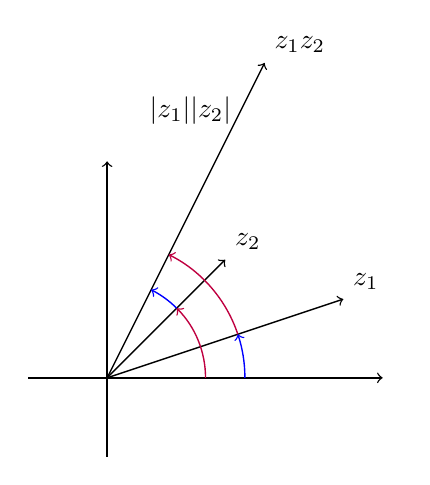
\begin{tikzpicture}
	\coordinate (origin) at (0,0);
	\coordinate (one) at (1.0, 0.0);
	\coordinate (im) at (0.0, 1.0);
	\coordinate (z1) at (3.0, 1.0);
	\coordinate (z2) at (1.5, 1.5);
	\coordinate (z) at (2, 4);

	% draw axes
	\draw [->] (-1, 0) -- (3.5, 0) node [right] {$\re$};
	\draw [->] (0, -1) -- (0, 2.75) node [above] {$\im$};

	% draw vectors
	\draw [->] (origin) -- (z1) node [anchor=south west] {$z_1$};
	\draw [->] (origin) -- (z2) node [anchor=south west] {$z_2$};
	\draw [->] (origin) -- (z) node [anchor=south west] {$z_1 z_2$} node [pos=0.85, anchor=east] {$|z_1|  |z_2|$};

	\pic [draw, ->, angle eccentricity=1.2, angle radius=1.75cm, color=blue] {angle = one--origin--z1};
	\pic [draw, ->, angle eccentricity=1.2, angle radius=1.75cm, color=purple] {angle = z1--origin--z};

	\pic [draw, ->, angle eccentricity=1.2, angle radius=1.25cm, color=purple] {angle = one--origin--z2};
	\pic [draw, ->, angle eccentricity=1.2, angle radius=1.25cm, color=blue] {angle = z2--origin--z};
	\end{tikzpicture}
  \end{center}

To see how useful a geometric perspective can be, consider the following result.

\begin{proposition}[Triangle Inequality]
	For complex numbers $z_1$ and $z_2$, $|z_1 + z_2| \leq |z_1| + |z_2|$.
\end{proposition}
\begin{proof}[Algebraic Proof]
	We have $|z_1 + z_2|^2 = (z_1 + z_2)\overline{(z_1 + z_2)} = |z_1|^2 + z_1 \overline{z_2} + \overline{z_1} z_2 + |z_2|^2$, so it suffices to show that $z_1 \overline{z_2} + \overline{z_1} z_2 \leq 2 |z_1| |z_2|$. To show this, we have
	\begin{align*}
		z_1 \overline{z_2} + \overline{z_1} z_2 &\leq 2 |z_1| |z_2| \\
\iff 	\frac{z_1 \overline{z_2} + \overline{z_1 \overline{z_2}}}{2} &\leq |z_1| |\overline{z_2}| \\
\iff \re(z_1 \overline{z_2}) &\leq |z_1 \overline{z_2}|,
	\end{align*}
	which is true. 
\end{proof}

Now put everything on an Argand diagram and stare at it for a minute.


\begin{center}
	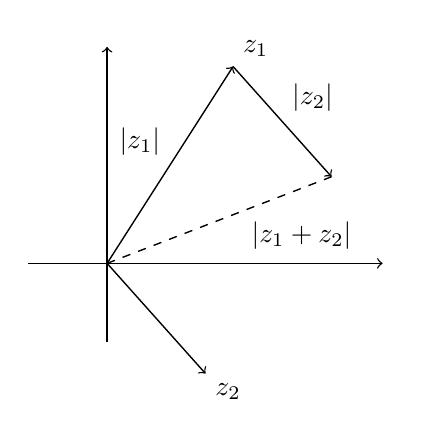
\begin{tikzpicture}
	\coordinate (origin) at (0,0);
	\coordinate (one) at (1.0, 0.0);
	\coordinate (im) at (0.0, 1.0);
	\coordinate (z1) at (1.6, 2.5);
	\coordinate (z2) at (1.25, -1.4);

	% draw axes
	\draw [->] (-1, 0) -- (3.5, 0) node [right] {$\re$};
	\draw [->] (0, -1) -- (0, 2.75) node [above] {$\im$};

	% draw vectors
	\draw [->] (origin) -- (z1) node [anchor=south west] {$z_1$} node [pos=0.5, anchor=south east] {$|z_1|$};
	\draw [->] (origin) -- (z2) node [anchor=north west] {$z_2$};
	\draw [dashed] (origin) -- (2.85, 1.1) node [pos=0.6, anchor=north west] {$|z_1 + z_2|$};
	\draw [->] (z1) -- (2.85, 1.1) node [pos=0.5, anchor=south west] {$|z_2|$};
	\end{tikzpicture}
  \end{center}

\begin{proof}[Geometric Proof]
	The shortest distance between $0$ and $z_1 + z_2$ is $|z_1 + z_2|$. This is a side length of the triangle at $0$, $z_1$ and $z_1 + z_2$, and this must be shorter than the other two sides of the triangle, which has length $|z_1| + |z_2|$. This gives the triangle inequality. 
\end{proof}

Alternate forms of the triangle inequality are
$$
|z_2 - z_1| \geq |z_2| - |z_1|, \quad \text{and} \quad |z_2  - z_1| \geq |z_1| - |z_2|.
$$
One of these tends to be trivially true, however, due to one side being negative. Still, we can combine these into a single statement
$$
|z_2 - z_1| \geq ||z_2| - |z_1||.
$$

We will end our discussion with the following theorem which will repeatedly appear.

\begin{theorem}[De Moivre's Theorem]
	For $n \in \Z$ and $\theta \in \R$, we have
	$$
	(\cos \theta + i \sin \theta)^n = \cos n \theta + i \sin n \theta,
	$$
	where $z^0 = 1$ for non-zero $z$.
\end{theorem}
\begin{proof}[Proof Sketch]
	Use induction and angle sum identities. A different proof will be given after exponential functions are defined.
\end{proof}

\subsection{Exponential and Trigonometric Functions}

We define the functions $\exp$, $\cos$ and $\sin$ on the complex numbers by
\begin{align*}
	\exp(z) &= \sum_{n = 0}^{\infty} \frac{1}{n!} z^n = e^z \\
	\cos(z) &= \frac{1}{2}(e^{iz} + e^{-iz}) = 1 - \frac{1}{2!}z^2 + \frac{1}{4!} z^4 - \cdots \\
	\sin(z) &= \frac{1}{2i}(e^{iz} - e^{-iz}) = z - \frac{1}{3!}z^3 + \frac{1}{5!}z^5 - \cdots
\end{align*}
These functions are defined by \vocab{power series}, which will be explored more in Analysis. They converge for all $z$, and can be manipulated and rearranged as you may expect.

\begin{aside}{Aside: Power Series (Preview of Analysis I)}

	A \vocab{power series} about a point $x_0$ is a sum of the form
	$$
	\sum_{n = 0}^{\infty} a_n(x - x_0)^n,	
	$$
	where $a_n \in \C$. A power series is said to \vocab{converge} at a point $x$ if the finite sums
	$
	\sum_{n = 0}^N a_n(x - x_0)^n
	$
	tend to a limit as $N \rightarrow \infty$. With each power series there is a \vocab{radius of convergence} $\rho$ such that if $\left|x-x_{0}\right|<\rho,$ then the power series converges absolutely. If $\left|x-x_{0}\right|>\rho,$ then the series does not converge. If $\left|x-x_{0}\right|=\rho,$ then it may or may not converge. In the functions defined above, the radius of convergence is infinity.


	We can manipulate power series as you might expect. Notably, we can differentiate term by term (and the radius of convergence will stay the same), and we can add and multiply power series if we are in the radius of convergence of both.

	Power series will be discussed in detail in Analysis I.
	
\end{aside}

These definitions reduce to familiar definitions when $z \in \R$. Indeed, if we differentiate the series, we get
$$
	\frac{\mathrm{d}}{\mathrm{d}x} \exp(x) = \exp(x), \quad
	\frac{\mathrm{d}}{\mathrm{d}x}\cos(x) = -\sin(x), \quad
	\frac{\mathrm{d}}{\mathrm{d}x} \sin(x) = \cos(x),
$$
and $\exp(0) = 1$, $\cos(0) = 1$, $\sin(0) = 0$, which together uniquely defines these functions over the reals. However, the behavior over $\C$ is somewhat richer.

\begin{proposition}[Properties of the Complex Exponential]
	For $z = x + yi$,
	\begin{enumerate}[label=(\roman*)]
		\item $e^z = e^x(\cos y + i \sin y)$.
		\item $e^z$ can take on all values in $\C$ except 0.
		\item $e^z = 1$ if and only if $z = 2 n \pi i$ for $n \in \Z$. 
	\end{enumerate}
\end{proposition}
\begin{proof}\begin{enumerate}[label=(\roman*)]
	\item $e^{x + iy} = e^x e^{iy}$, and $e^{iy} = \cos y + i \sin y$.
	\item $|e^z| = |e^x|$, which takes on all positive real values, and $\arg(e^z) = y$, which takes on all real values.
	\item $e^z = 1 \iff e^x = 1$ and $\cos y = 1$, $\sin y = 0$ which gives $x = 0$ and $y = 2 n \pi$ as required. \qedhere
\end{enumerate}
\end{proof}

Returning to polar form, we can write
$$
z = r(\cos \theta + i \sin \theta) = re^{i \theta},
$$
where $r = |z|$ and $\theta = \arg(z)$. 
Then De Moivre's theorem follows immediately from $(e^{i \theta})^n = e^{i n \theta}$.


\subsection{Roots of Unity}

An important application of these results are \emph{roots of unity}, which answers the question `find all $z$ such that $z^n = 1$'.

\begin{definition}[Roots of Unity]
	An \vocab{$n$th root of unity} is a complex number $z$ such that $z^n = 1$.
\end{definition}

\begin{proposition}[Finding Roots of Unity]
	The $n$th roots of unity are
	$$
	z = e^{2 k \pi i / n} = \cos \frac{2 \pi k}{n}+ i \sin \frac{2 \pi k}{n},
	$$
	where $k \in \{0, 1, \dots, n - 1\}$.
\end{proposition}
\begin{proof}
	Writing $z$ in polar form, these are easy to find. We have $z = re^{i \theta}$, then
$$
z^n = r^n e^{i n \theta} = 1,
$$
so $r = 1$, and $\theta = \frac{2 k \pi}{n}$ for some $k \in \Z$. This gives $n$ distinct solutions.
\end{proof}

To get a feel for this, we can plot the cases for $n = 2, 3, 4$ and $5$ on an Argand diagram. This hints at a geometric interpretation of the roots of unity.

\begin{figure}[h]  
	\centering 
	\begin{subfigure}[b]{0.4\linewidth}
		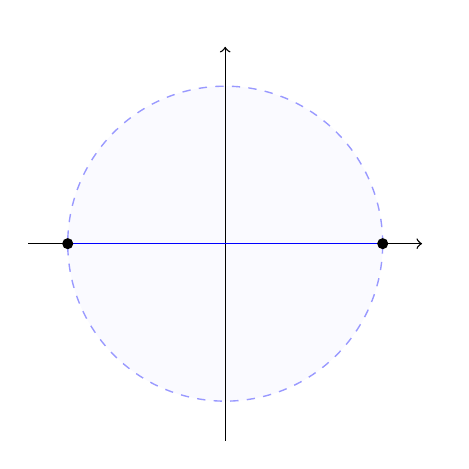
\begin{tikzpicture}
			\coordinate (origin) at (0,0);
			\coordinate (one) at (1.0, 0.0);
			\coordinate (im) at (0.0, 1.0);
		
			\filldraw[dashed, color=blue!40, fill=blue!2] (0, 0) circle (2);

			% draw axes
			\draw [->] (-2.5, 0) -- (2.5, 0) node [right] {$\re$};
			\draw [->] (0, -2.5) -- (0, 2.5) node [above] {$\im$};
		
			\draw [color=blue] (2,0) --(-2, 0);

			% points
			\fill (2,0)  circle[radius=2pt];
			\fill (-2,0)  circle[radius=2pt];
			\end{tikzpicture}
		\caption{$n = 2$}
	  \end{subfigure}
	  \begin{subfigure}[b]{0.4\linewidth}
		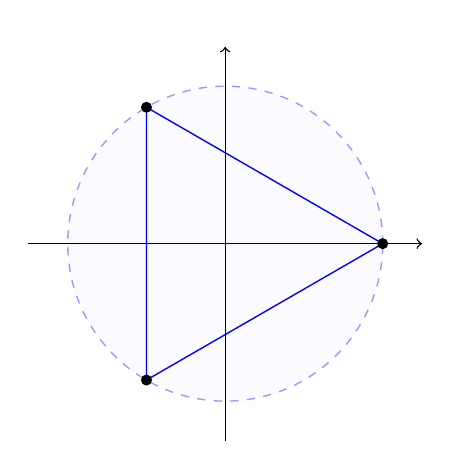
\begin{tikzpicture}
			\coordinate (origin) at (0,0);
			\coordinate (one) at (1.0, 0.0);
			\coordinate (im) at (0.0, 1.0);
			\coordinate (p1) at (2,0);
			\coordinate (p2) at (-1,-1.73206);
			\coordinate (p3) at (-1, 1.73206);
		
			\filldraw[dashed, color=blue!40, fill=blue!2] (0, 0) circle (2);

			\draw [color=blue] (p1) -- (p2) -- (p3) -- (p1);

			% draw axes
			\draw [->] (-2.5, 0) -- (2.5, 0) node [right] {$\re$};
			\draw [->] (0, -2.5) -- (0, 2.5) node [above] {$\im$};
		
			% points
			\fill (p1)  circle[radius=2pt];
			\fill (p2)  circle[radius=2pt];
			\fill (p3)  circle[radius=2pt];
			\end{tikzpicture}%
		\caption{$n = 3$}
	  \end{subfigure}
	\begin{subfigure}[b]{0.4\linewidth}
		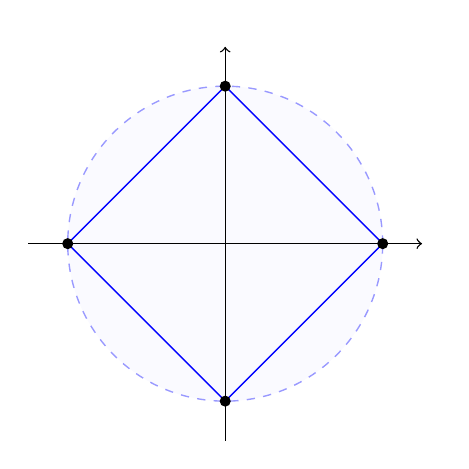
\begin{tikzpicture}
			\coordinate (origin) at (0,0);
			\coordinate (one) at (1.0, 0.0);
			\coordinate (im) at (0.0, 1.0);
			\coordinate (p1) at (2,0);
			\coordinate (p2) at (0,2);
			\coordinate (p3) at (-2,0);
			\coordinate (p4) at (0,-2);
		
			\filldraw[dashed, color=blue!40, fill=blue!2] (0, 0) circle (2);

			\draw [color=blue] (p1) -- (p2) -- (p3) -- (p4) -- (p1);

			% draw axes
			\draw [->] (-2.5, 0) -- (2.5, 0) node [right] {$\re$};
			\draw [->] (0, -2.5) -- (0, 2.5) node [above] {$\im$};
		
			% points
			\fill (p1)  circle[radius=2pt];
			\fill (p2)  circle[radius=2pt];
			\fill (p3)  circle[radius=2pt];
			\fill (p4)  circle[radius=2pt];
			\end{tikzpicture}
	\caption{$n = 4$}
	\end{subfigure}
	\begin{subfigure}[b]{0.4\linewidth}
		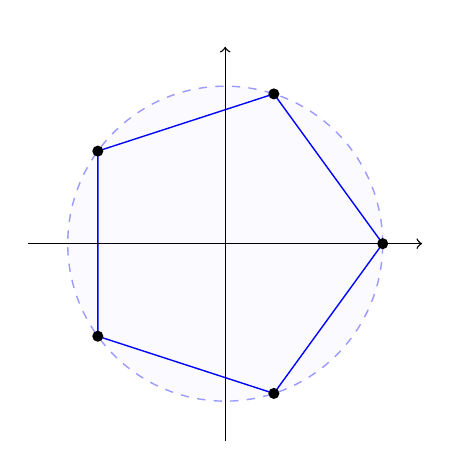
\begin{tikzpicture}
			\coordinate (origin) at (0,0);
			\coordinate (one) at (1.0, 0.0);
			\coordinate (im) at (0.0, 1.0);
			\coordinate (p1) at (2,0);
			\coordinate (p4) at (-1.6180,-1.1756);
			\coordinate (p2) at (0.6180,1.9021);
			\coordinate (p5) at (0.6180,-1.9021);
			\coordinate (p3) at (-1.6180,1.1756);

			\filldraw[dashed, color=blue!40, fill=blue!2] (0, 0) circle (2);

			\draw [color=blue] (p1) -- (p2) -- (p3) -- (p4) -- (p5) -- (p1);

			% draw axes
			\draw [->] (-2.5, 0) -- (2.5, 0) node [right] {$\re$};
			\draw [->] (0, -2.5) -- (0, 2.5) node [above] {$\im$};
		
			% points
			\fill (p1)  circle[radius=2pt];
			\fill (p2)  circle[radius=2pt];
			\fill (p3)  circle[radius=2pt];
			\fill (p4)  circle[radius=2pt];
			\fill (p5)  circle[radius=2pt];
			\end{tikzpicture}
	\caption{$n = 5$}
	\end{subfigure}
	\caption{$n$th roots of unity on an Argand diagram}
	\end{figure}  

	\begin{proposition}[Geometric Interpretation of Roots of Unity]
		The $n$th roots of unity correspond to the vertices of a regular $n$-gon, inscribed within the unit circle with a vertex at $1$.
	\end{proposition}
	\begin{proof}
		Follows directly from roots of unity written in polar form.
	\end{proof}

\subsection{Logarithms and Complex Powers}

Over $\R$, the exponential function is one to one. This means that we can quite easily define the inverse function, the logarithm, on the positive reals (the image of the exponential over $\R$).

This is not true over $\C$, as the complex exponential function is many to one. For example, $e^{3\pi i/2} = e^{7 \pi i/2} = -i$. However, we do know that if we have $e^{i\theta} = e^{i \gamma}$, then $\theta$ and $\gamma$ differ by a multiple of $2 \pi$\footnote{This comes from the argument of a complex number only being defined up to a multiple of $2\pi$}. Thus we can define a \emph{multi-valued} logarithm function.

\subsubsection{The Complex Logarithm}

To see how to define the logarithm over $\C$, let $z$ be any non-zero complex number. Then if we let $\theta = \arg(z)$ with $-\pi < \theta \leq \pi$, then we can write
$$
z = re^{i \theta} =  e^{\log r} e^{i \theta + 2n \pi i} = e^{\log r + i(\theta + 2n \pi)},
$$
for any $n \in \Z$.

\begin{definition}[Complex Logarithm]
	For a complex number $z$, we define the \vocab{complex logarithm} $\log z$ to be the multi-valued function
	$$
	\log z = \log r + i(\theta + 2n\pi),
	$$
	where $r = |z|$, $\theta = \arg (z)$ with $- \pi < \theta \leq \pi$ and $n \in \Z$.
\end{definition}

\begin{example}[Calculating Complex Logarithms]
	Let $z = \frac{5}{2} + \frac{5\sqrt{3} i}{2}$. We will find $\log z$. We have $|z| = 5$, and the principal value is $\arg(z) = \pi/3$. Thus we have
	$$
	\log z = \log 5 + i (\pi/3 + 2n \pi), \quad n \in \mathbb{Z}.
	$$
\end{example}

Sometimes we will want single-valued behavior from the complex logarithm, and we can define the \vocab{principal logarithm} so that we fix $n = 0$. A warning though: if this is done, not all of the familiar properties of the logarithm still hold.\footnote{When taking the principal logarithm, we are really taking a \emph{branch} of the multi-valued logarithm function. This corresponds with taking a slice of the Riemann surface that $\log z$ defines. This gives some weird behavior as we move past certain sets of points (singular points) which breaks many of the identities that we use frequently for the real valued logarithm.}

\subsubsection{Complex Powers}

The multi-valued nature of the logarithm carries into the notion of taking powers of complex numbers.
For real numbers, we can define $x^a = e^{a \ln x}$ for $x > 0$. We can do the same for complex numbers.

\begin{definition}[Complex Powers]
	We define \vocab{complex powers} for $z, \alpha \in \C$ with $z \neq 0$ to be the multi-valued
	$$
	z^{\alpha} = e^{\alpha \log z}.
	$$
\end{definition}

This is not \emph{always} multi valued. For example, if $\alpha \in \Z$, then $z^\alpha$ is unique. If $\alpha \in \Q$, then there will be only finitely many values. However, in most cases there will be infinitely many values.

\begin{example}[Calculating $i^i$]
	We have
	\begin{align*}
		i^i &= e^{i \log i} \\
		&= e^{i \log 1 + i(\pi/2 + 2n\pi)} \\
		&= e^{-(2n + 1/2)\pi},
	\end{align*}
	for any $n \in \Z$. Notably $i^i \in \R$.
\end{example}


\subsection{Transformations, Lines and Circles}

Consider the following transformations on $\C$.
\begin{itemize}
	\item $z \mapsto z + \alpha$, translation by $\alpha \in \C$.
	\item $z \mapsto \lambda z$, scaling by $\lambda \in \R$,
	\item $z \mapsto e^{i \theta} z$, rotation by $\theta \in \R$. 
	\item $z \mapsto \overline{z}$, reflection in the real axis.
	\item $z \mapsto \frac{1}{z}$, inversion.
\end{itemize}
Using these transformations, we can think geometrically to do things like find equations of various geometric objects.

First we will find the general point on a line
in $\C$ through $z_0$, parallel to $w \in \C$ where $w \neq 0$.
\begin{center}
	\begin{tikzpicture}
		\coordinate (origin) at (0,0);
		\coordinate (one) at (1.0, 0.0);
		\coordinate (im) at (0.0, 1.0);
		\coordinate (z1) at (1, 0.33);
		\coordinate (z2) at (-0.8, 1.4);
	
		% draw axes
		\draw [->] (-1, 0) -- (3.5, 0) node [right] {$\re$};
		\draw [->] (0, -1) -- (0, 2.75) node [above] {$\im$};
	
		% draw vectors
		\draw [->] (origin) -- (z1) node [anchor=south west] {$w$};
		\draw [->] (origin) -- (z2) node [anchor=south west] {$z_0$};
		\draw [<->, dashed, color=blue!80] ($(z2) - (z1)$) -- ($(z2) + (z1) + (z1) + (z1) + (z1) + (z1)$);
		\fill ($(z2) + (z1) + (z1)$)  circle[radius=2pt] node [anchor=south west] {$z$};
	\end{tikzpicture}
\end{center}
We can write $z = z_0 + \lambda w$ for $\lambda \in \R$. To eliminate $\lambda$, we can take the conjugate $\overline{z} = \overline{z_0} + \lambda \overline{w}$, and then multiplying by $w$ and subtracting we obtain $\overline{w}z - w\overline{z} = \overline{w} z_0 - w \overline{z_0}$.

Similarly, we can find the general point on a circle with a center $c \in \C$ and positive real radius $\rho$.

\begin{center}
	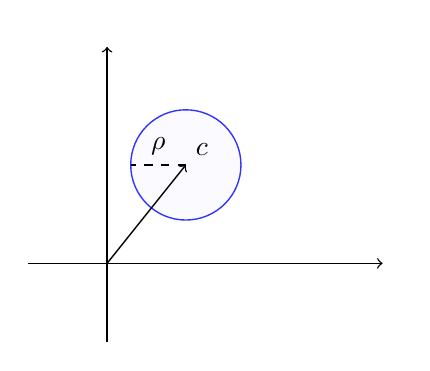
\begin{tikzpicture}
		\coordinate (origin) at (0,0);
		\coordinate (one) at (1.0, 0.0);
		\coordinate (im) at (0.0, 1.0);
		\coordinate (z1) at (1, 1.25);
		% \coordinate (z2) at (-0.8, 1.4);
	
		
		\filldraw[color=blue!80, fill=blue!2] (z1) circle (0.7);

		% draw axes
		\draw [->] (-1, 0) -- (3.5, 0) node [right] {$\re$};
		\draw [->] (0, -1) -- (0, 2.75) node [above] {$\im$};
	
		% draw vectors
		\draw [->] (origin) -- (z1) node [anchor=south west] {$c$};
		\draw [dashed] (1, 1.25) -- (0.3, 1.25) node [pos=0.5, anchor=south] {$\rho$};
		\end{tikzpicture}
\end{center}
A general point on this circle can be written $z = c + \rho e^{i \alpha}$, $\alpha \in \R$. To get rid of $\alpha$, note that we could instead write $|z - c| = \rho$.

We can unify these two forms in the following way.

\begin{proposition}[Circles and Lines in $\C$]
	The equation of any line, and of any circle, may be written respectively as
$$
\bar{B} z+ B \bar{z}+C=0 \quad \text { and } \quad z \bar{z}+\bar{B} z+B \bar{z}+C=0
$$
for some complex $B$ and real $C$.

In particular, the first is a line in the direction $iB$, and the second (if $|B|^2 > C$) is a circle with centre $-B$ and radius $\sqrt{|B|^2 - C}$.
\end{proposition}
\begin{proof}
	For the line, we found above that a general line through $z_0$ parallel to $w$ satisfies $\overline{w}z - w\overline{z} = \overline{w}z_0 - w\overline{z_0}$. The right-hand side is a constant, and both sides are purely imaginary (each is equal to the negative of its own conjugate). Multiplying through by $i$, we can write this as $\overline{B}z + B\overline{z} + C = 0$ where $B = -iw$ and $C \in \R$, and then the direction of the line is $w = iB$ (rescaling to absorb factors). This process is reversible, so every equation of this form with $B \neq 0$ gives a line.

	For the circle, expanding $|z - c|^2 = \rho^2$ gives
	$$
	z\bar{z} - \bar{c}z - c\bar{z} + |c|^2 - \rho^2 = 0,
	$$
	which is of the stated form with $B = -c$ and $C = |c|^2 - \rho^2 \in \R$. Conversely, given such an equation we can complete the square to get $|z + B|^2 = |B|^2 - C$, a circle with centre $-B$ and radius $\sqrt{|B|^2 - C}$, provided $|B|^2 > C$.
\end{proof}


\section{Vectors in Three Dimensions}

Fundamentally, vectors are mathematical objects that we can add together and take multiples of, in both cases obtaining another vector. We will consider vectors in a general setting later on, but in this chapter we will consider vectors in $\R^3$, three dimensional space. Specifically, we will take a geometric approach, thinking of vectors as position vectors and using Euclidean notions of points, lines, planes, etc.

We begin by choosing a point $O$ as the origin. Then points $A$ and $B$ have position vectors
$$
\vv{a} = \overrightarrow{OA}, \quad\quad \vv{b} = \overrightarrow{OB}.
$$

\begin{center}
	\begin{tikzpicture}
	\coordinate (origin) at (0,0);
	\coordinate (a) at (4, 0.25);
	\coordinate (b) at (1.5, 2.25);

	\draw (origin) node [anchor=north east] {$O$};

	\draw [->,>=stealth] (origin) -- (a) node [anchor=north west] {$A$} node [pos=0.6, anchor=north] {$\vv{a}$};
	\draw [->,>=stealth] (origin) -- (b) node [anchor=north west] {$B$} node [pos=0.6, anchor=north west] {$\vv{b}$};
	\end{tikzpicture}
\end{center}

The vectors have length $|\vv{a}| = |\overrightarrow{OA}|$, the distance between $O$ and $A$. We also let $\vv{0}$ denote the position vector of $O$.

\subsection{Vector Addition and Scalar Multiplication}

The most important operations on vectors (in $\R^3$ and in general) are vector addition and scalar multiplication. We define these geometrically as follows.

\begin{definition}[Scalar Multiplication in $\R^3$]
	Given $\vv{a}$, the position vector for a point $A$, and a scalar $\lambda \in \R$, we define \vocab{scalar multiplication} $\lambda \vv{a}$ to be the position vector for the point $A'$ on the line $OA$ such that
	$$
	|\lambda \vv{a} | = |OA'| = |\lambda| |\vv{a}|,
	$$
	with the vector being in the direction $\overrightarrow{OA}$ if $\lambda$ is positive, and in the opposite direction otherwise.
\end{definition}

\begin{center}
	\begin{tikzpicture}
	\coordinate (origin) at (0,0);
	\coordinate (a) at (2, 0.17);

	\draw (origin) node [anchor=north east] {$O$};

	\draw [->,>=stealth, dashed] ($(origin)  - (a) - (a)$) -- ($(a) + (a) + (a) + (a) $);

	\draw [->,>=stealth, color=blue] (origin) -- ($(a) + (a) + (a)$) node [anchor=north west, color=black] {$A'$} node [pos=0.8, anchor=north] {$\lambda\vv{a}$};
	\draw [->,>=stealth, color=black] (origin) -- ($(a)$) node [anchor=north west, color=black] {$A$} node [pos=0.6, anchor=north, color=black] {$\vv{a}$};
	
	\end{tikzpicture}
\end{center}

If two vectors are scalar multiples of each other, then we say that they are \vocab{parallel}. Specifically, we write $\vv{a} \parallel \vv{b}$ if and only if $\vv{a} = \lambda \vv{b}$ or $\vv{b} = \lambda \vv{a}$ for some $\lambda \in \R$. Notably, $\vv{a} \parallel \vv{0}$ for all vectors $\vv{a}$.


\begin{definition}[Vector Addition in $\R^3$]
	Given $\vv{a}$ and $\vv{b}$, position vectors of points $A$ and $B$, if $\vv{a} \not \parallel \vv{b}$, we construct the parallelogram $OACB$, and define \vocab{vector addition} $\vv{a} + \vv{b} = \vv{c}$. 
\end{definition}


\begin{center}
	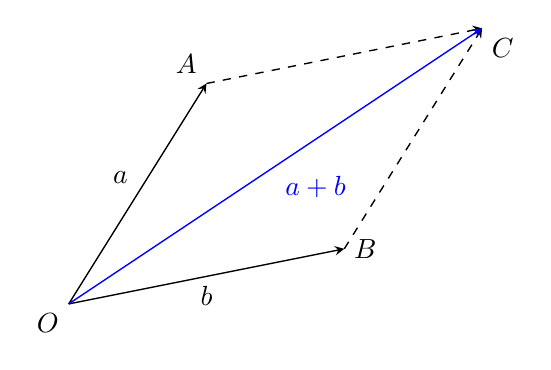
\begin{tikzpicture}[xscale=1.4, yscale=1.4]
	\draw (0, 0) node [anchor=north east] {$O$};
	\draw [->,>=stealth] (0, 0) -- (2.5, 0.5) node [anchor=west] {$B$} node [pos=0.5, anchor=north] {$\vv{b}$};
	\draw [->,>=stealth] (0, 0) -- (1.25, 2.0) node [anchor=south east] {$A$} node [pos=0.5, anchor=south east] {$\vv{a}$};
	\draw [->,>=stealth, dashed] (1.25, 2.0) -- (3.75, 2.5);
	\draw [->,>=stealth, dashed] (2.5, 0.5) -- (3.75, 2.5);
	\draw [->,>=stealth, color=blue] (0,0) -- (3.75, 2.5) node [pos=0.5, anchor=north west] {$\vv{a} + \vv{b}$};
	\draw (3.75, 2.5) node [anchor=north west] {$C$};
	\end{tikzpicture}
  \end{center}

If $\vv{a} \parallel \vv{b}$, then writing $\vv{a} = \alpha \vv{u}$ and $\vv{b} = \beta \vv{u}$ where $\vv{u}$ is a unit vector, then $\vv{a} + \vv{b} = (\alpha+ \beta) \vv{u}$.

Given some set of vectors $\vv{v_1}$, $\vv{v_2}$, $\dots$, $\vv{v_k}$, we can form a \vocab{linear combination}
$$
\lambda_1 \vv{v_1} + \lambda_2 \vv{v_2}  + \cdots + \lambda_k \vv{v_k},
$$
where $\lambda_i \in \R$. With this in mind, we can consider the set of all vectors that can be formed as a linear combination of some vectors.

\begin{definition}[Span]
	For vectors $\vv{v_1}$, $\vv{v_2}$, $\dots$, $\vv{v_k}$, we define their \vocab{span} to be the set
	$$
	\vecspan\{\vv{v_1}, \vv{v_2}, \dots, \vv{v_k} \} = \{ \lambda_1 \vv{v_1} + \lambda_2 \vv{v_2}  + \cdots + \lambda_k \vv{v_k} \mid \lambda_i \in \R \}.
	$$
\end{definition}

If two vectors $\vv{a} \not \parallel \vv{b}$, then $\vecspan\{\vv{a}, \vv{b}\}$ is a plane through $OAB$.

Vector addition and scalar multiplication obey some basic properties that you should keep in mind, as they will be used again when we define vectors in a general sense.

\begin{proposition}[Basic Properties of Vector Operations]
For any vectors $\vv{a}$, $\vv{b}$ and $\vv{c}$,
\begin{enumerate}[label=(\roman*)]
	\item Vectors along with vector addition form an abelian group.
	\item $\lambda(\vv{a} + \vv{b}) = \lambda \vv{a} + \lambda \vv{b}$.
	\item $(\lambda + \mu)\vv{a} = \lambda\vv{a} + \mu\vv{a}$.
	\item $\lambda(\mu \vv{a}) = (\lambda \mu) \vv{a}$.
\end{enumerate}
\end{proposition}
\begin{proof}[Proof Sketch]
	Check geometric definitions. Checking associativity of vector addition will require the construction of a parallelepiped.
\end{proof}


\subsection{The Dot Product}

We saw in the previous section how to add vectors, and how to multiply a vector by a scalar. In the next two sections, we will consider how to multiply a vector and a vector. 
We will first define the \emph{scalar} or \emph{dot product}.
Consider two vectors $\vv{a}$ and $\vv{b}$, with the angle between then being $\theta$ as shown.

\begin{center}
    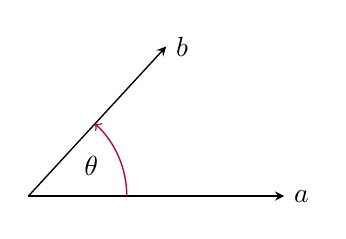
\begin{tikzpicture}
        \coordinate (origin) at (0,0);
        \coordinate (z) at (1.75, 1.9);
        \coordinate (z1) at (3.25, 0);

        % \draw (0, 0) node [anchor=north east] {$O$};
        \draw [->,>=stealth] (0, 0) -- (z1) node [anchor=west] {$\vv{a}$};
        %  node [pos=0.5, anchor=north] {$\vv{a}$};
        \draw [->,>=stealth] (0, 0) -- (z) node [anchor=west] {$\vv{b}$};
        %  node [pos=0.5, anchor=south east] {$\vv{b}$};
        \pic [draw, ->, angle eccentricity=1.2, angle radius=1.25cm, color=purple] {angle = z1--origin--z};
        \draw (0.8, 0.38) node {$\theta$};
	\end{tikzpicture}
  \end{center}

\begin{definition}[Dot Product]
    For two vectors $\vv{a}$ and $\vv{b}$, and $\theta$ the angle between them as shown, we define the \vocab{scalar} or \vocab{dot product} as
    $$
    \vv{a} \cdot \vv{b} = |\vv{a}| |\vv{b}| \cos \theta.
    $$

    [Note that $\theta$ is defined unless $\vv{a}$ or $\vv{b}$ is zero, but then $|\vv{a}| = 0$ or $|\vv{b}| = 0$ and $\vv{a} \cdot \vv{b} = 0$.]
\end{definition}

The scalar product encodes the angle between vectors, and in particular it gives us a test for perpendicularity. We say vectors $\vv{a}$ and $\vv{b}$ are \vocab{orthogonal} or \vocab{perpendicular} if and only if $\vv{a} \cdot \vv{b} = 0$. This corresponds with $\theta = \pm \pi/2$, or with either $|\vv{a}| = 0$ or $|\vv{b}| = 0$.

There is a geometric interpretation of the dot product. Fundamentally, the dot product is a \emph{projection}. For $\vv{a} \neq \vv{0}$, the quantity $|\vv{b}| \cos \theta$ is the component of $\vv{b}$ when projected along the direction of $\vv{a}$.

\begin{center}
    \begin{tikzpicture}
        \coordinate (origin) at (0,0);
        \coordinate (z) at (1.75, 1.9);
        \coordinate (z1) at (3.25, 0);

        \draw [dashed] (0, 0) -- (5.25, 0);

        \draw [color=blue, dashed] (z) -- (1.75, 0);

        \fill (1.75,0)  circle[color=blue, radius=1pt];

        % \draw (0, 0) node [anchor=north east] {$O$};
        \draw [->,>=stealth] (0, 0) -- (z1) node [anchor=north] {$\vv{a}$};
        %  node [pos=0.5, anchor=north] {$\vv{a}$};
        \draw [->,>=stealth] (0, 0) -- (z) node [anchor=west] {$\vv{b}$};
        %  node [pos=0.5, anchor=south east] {$\vv{b}$};
        \pic [draw, ->, angle eccentricity=1.2, angle radius=0.8cm, color=purple] {angle = z1--origin--z};
        \draw (0.533333333, 0.253333333) node {\small $\theta$};

        % \draw (1.75, 0) node [anchor=north] {$\vv{b}_{\parallel}$};
        \draw [color=blue] (0,0) -- (1.75, 0);

        \draw [decoration={brace, mirror, raise=0.4cm}, decorate] (0,0) -- (1.75, 0) node [pos=0.5, anchor=north, yshift=-0.45cm] {\footnotesize $|\vv{b}| \cos \theta$};
        \draw [densely dashed] (0,0) -- (0, -0.4cm);
        \draw [densely dashed] (1.75,0) -- (1.75, -0.4cm);
	\end{tikzpicture}
  \end{center}

  \begin{proposition}[Basic Properties of the Dot Product]
      For any vectors $\vv{a}$ and $\vv{b}$,
      \begin{enumerate}[label=(\roman*)]
          \item $\vv{a} \cdot \vv{b} = \vv{b} \cdot \vv{a}$.
          \item $\vv{a} \cdot \vv{a} = |\vv{a}|^2 \geq 0$, and $\vv{a} \cdot \vv{a} = 0$ if and only if $\vv{a} = \vv{0}$.
          \item $(\lambda \vv{a}) \cdot \vv{b} = \lambda (\vv{a} \cdot \vv{b}) = \vv{a} \cdot (\lambda \vv{b})$.
          \item $\vv{a} \cdot (\vv{b} + \vv{c}) = \vv{a} \cdot \vv{b} + \vv{a} \cdot \vv{c}$. 
      \end{enumerate}
  \end{proposition}
  \begin{proof}
      Properties (i) to (iii) follow directly from the definition of the dot product. Property (iv) follows from the geometric interpretation of the dot product shown above. 
  \end{proof}



\subsection{The Cross Product}

The next operation only works with vectors in three dimensions, and is the \emph{vector} or \emph{cross product}. As before, consider two vectors $\vv{a}$ and $\vv{b}$, and let $\theta$ be measured as shown with respect to $\hat{\vv{n}}$, a unit normal to the plane spanned by $\vv{a}$ and $\vv{b}$.

\begin{center}
    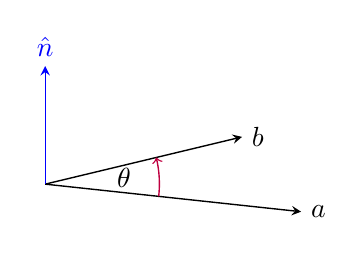
\begin{tikzpicture}
        \coordinate (origin) at (0,0);
        \coordinate (z) at (2.5, 0.6);
        \coordinate (z1) at (3.25, -0.35);

        % \draw (0, 0) node [anchor=north east] {$O$};
        \draw [->,>=stealth] (0, 0) -- (z1) node [anchor=west] {$\vv{a}$};
        %  node [pos=0.5, anchor=north] {$\vv{a}$};
        \draw [->,>=stealth] (0, 0) -- (z) node [anchor=west] {$\vv{b}$};
        %  node [pos=0.5, anchor=south east] {$\vv{b}$};
        \pic [draw, ->, angle eccentricity=1.8, angle radius=1.45cm, color=purple] {angle = z1--origin--z};
        
        \draw (1, 0.08) node {$\theta$};

        \draw [->,>=stealth, color=blue] (0,0) -- (0, 1.5) node [anchor=south] {$\hat{\vv{n}}$};
	\end{tikzpicture}
  \end{center}

  \begin{definition}[Cross Product]
For two vectors $\vv{a}$ and $\vv{b}$ with angle  $\theta$ measured as shown, we define the \vocab{vector} or \vocab{cross product} as
$$
\vv{a} \times \vv{b} = | \vv{a}| |\vv{b}| \sin \theta \hat{\vv{n}},
$$
where $\hat{\vv{n}}$ is a unit vector perpendicular to the plane spanned by $\vv{a}$ and $\vv{b}$.

[$\hat{\vv{n}}$ is defined up to a sign if $\vv{a} \not \parallel \vv{b}$, but changing the sign changes $\theta$ to $2\pi - \theta$, and thus leaves $\vv{a} \times \vv{b}$ unchanged. When $\hat{\vv{n}}$ is not defined ($\vv{a} \parallel \vv{b}$ or $\theta$ not defined), $\vv{a} \times \vv{b} = \vv{0}$.] 
  \end{definition}

  The geometric interpretation of the cross product is that $|\vv{a} \times \vv{b}|$ is the area of the parallelogram as shown.

  \begin{center}
    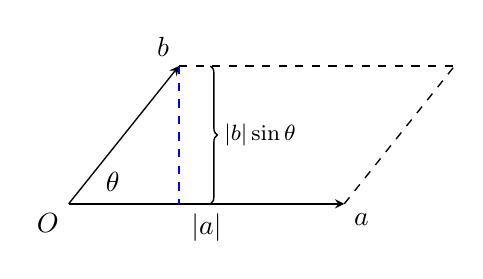
\begin{tikzpicture}[xscale=1.4, yscale=1.4]
    \draw (0, 0) node [anchor=north east] {$O$};
    
    \draw [->,>=stealth] (0, 0) -- (2.5, 0) node [anchor=north west] {$\vv{a}$} node [pos=0.5, anchor=north] {$|\vv{a}|$};
    \draw [->,>=stealth] (0, 0) -- (1, 1.25) node [anchor=south east] {$\vv{b}$};

    \draw (0.4, 0.2) node {$\theta$};

    \draw [dashed] (1, 1.25) -- (3.5, 1.25);
    \draw [dashed] (2.5, 0) -- (3.5, 1.25);

    \draw [dashed, color=blue] (1,1.25) -- (1, 0);
    \draw [decoration={brace, raise=0.4cm}, decorate] (1, 1.25) -- (1, 0) node [pos=0.5, anchor=west, xshift=0.45cm] {\footnotesize $|\vv{b}| \sin \theta$};
    
	% \draw [->,>=stealth, dashed] (1.25, 2.0) -- (3.75, 2.5);
	% \draw [->,>=stealth, dashed] (2.5, 0.5) -- (3.75, 2.5);
	% \draw [->,>=stealth, color=blue] (0,0) -- (3.75, 2.5) node [pos=0.5, anchor=north west] {$\vv{a} + \vv{b}$};
	% \draw (3.75, 2.5) node [anchor=north west] {$C$};
    \end{tikzpicture}
  \end{center}

  The direction of $\vv{a} \times \vv{b}$ gives the orientation of this parallelogram in space.   

For an alternate geometric interpretation, fix a vector $\vv{a}$ and consider some vector $\vv{x}$ with $\vv{x} \perp \vv{a}$. Then the transformation $\vv{x} \longmapsto \vv{a} \times \vv{x}$ corresponds with scaling $\vv{x}$ by $|\vv{a}|$ and rotating by $\pi/2$ in the plane perpendicular to $\vv{a}$.

\begin{proposition}[Basic Properties of the Cross Product]
    For vectors $\vv{a}$, $\vv{b}$ and $\vv{c}$,
    \begin{enumerate}[label=(\roman*)]
        \item $\vv{a} \times \vv{b} = - (\vv{b} \times \vv{a})$.
        \item $(\lambda \vv{a}) \times \vv{b} = \lambda (\vv{a} \times \vv{b})$.
        \item $\vv{a} \times (\vv{b} + \vv{c}) = \vv{a} \times \vv{b} + \vv{a} \times \vv{c}$.
        \item $\vv{a} \times \vv{b} = \vv{0}$ if and only if $\vv{a} \parallel \vv{b}$.
        \item $\vv{a} \times \vv{b} \perp \vv{a}, \vv{b}$, so $\vv{a} \cdot (\vv{a} \times \vv{b}) = \vv{b} \cdot (\vv{a} \times \vv{b}) = 0$. 
    \end{enumerate}
\end{proposition}
\begin{proof}[Proof Sketch]
    Check definitions.
\end{proof}

\subsection{Orthonormal Bases and Components}

So far we have considered vectors in a purely geometric sense. But just as a coordinate system can be used to reason about geometry, basis (and by extension components) can be used to reason about vectors. We will look at bases again in a more general setting later on, but for now we will focus on vectors in three dimensions.

When we use a cartesian coordinate system, we pick a set of axes and using them, we can describe the position of any point. In a similar way, a \emph{basis} is a set of vectors that span the space. That is, any vector can be written as a linear combination of vectors in the set. However we also have an additional requirement: this linear combination must be unique.

\begin{definition}[Basis -- Informal]
    We say that a set of vectors is a \vocab{basis} if any vector can be uniquely written as a linear combination of vectors in the set.
\end{definition}

Before we continue, it's helpful when working with vectors in three dimensions (and in other settings) to pick basis vectors in a certain way. We introduce the following definition.

\begin{definition}[Orthonormal]
    We say that a set of vectors $\{\vv{v_1}, \vv{v_2}, \dots, \vv{v_n} \}$ is \vocab{orthonormal} if they are all unit vectors and are orthogonal to each other. That is, if $|\vv{v_i}| = 1$ and
    $$
        \vv{v_i} \cdot \vv{v_j} = \begin{cases}
            1 &\mbox{if } i = j, \\
            0 &\mbox{if } i \neq j.
           \end{cases}
    $$
    for all $1 \leq i, j \leq n$.
\end{definition}

Now choose vectors $\vv{e}_1, \vv{e}_2, \vv{e}_3$ that are \vocab{orthonormal}. Then the set $\{\vv{e}_i \}$ is a basis, so for any vector $\vv{a}$, we can write
$$
\vv{a} = \sum_{i} a_i \vv{e}_i = a_1 \vv{e}_1 + a_2 \vv{e}_2 + a_3 \vv{e}_3,
$$
and each coefficient is uniquely defined by $a_i = \vv{e}_i \cdot \vv{a}$. Note that this only works because of our orthonormal condition.

Recalling that dot products correspond to projections, we can see that this really is analogous to a cartesian coordinate system.

\begin{center}
    \begin{tikzpicture}
        \draw [->,>=stealth] (0, 0) -- (0, 2) node [anchor=south] {$\vv{e}_3$};
        \draw [->,>=stealth] (0, 0) -- (1.95, -0.4) node [anchor=west] {$\vv{e}_2$};
        \draw [->,>=stealth] (0, 0) -- (-1.45, -1) node [anchor=north east] {$\vv{e}_1$};

        \draw [dashed, color=blue] (0.85, 1.6) -- (0, 1.675);

        \draw [->,>=stealth, color=red] (0, 0) -- (0.85, 1.6) node [anchor=south west] {$\vv{a}$};

        \draw [decoration={brace, raise=0.25cm}, decorate, color=blue] (0,0) -- (0, 1.675) node [pos=0.5, anchor=east, xshift=-0.3cm] {\footnotesize $a_3$}; 
    \end{tikzpicture}
\end{center}
Once we have specified the basis vectors $\{\vv{e}_i\}$, we can then identify the vector $\vv{a}$ by its \vocab{components}, writing 
$$
\vv{a} = (a_1, a_2, a_3), \quad \quad \text{or} \quad \quad \vv{a} = \begin{pmatrix} a_1 \\ a_2 \\ a_3 \end{pmatrix},
$$
which is a \vocab{row} or \vocab{column} vector respectively\footnote{The difference will be important when we move onto matrices.}.

An advantage of writing vectors in this form is that we can work directly with the components of vectors, rather than using a purely geometric approach.

\subsubsection{Dot Product in Components}

For two vectors $\vv{a} = (a_1, a_2, a_3)$ and $\vv{b} = (b_1, b_2, b_3)$, their dot product is
$$
\vv{a} \cdot \vv{b} = (a_1, a_2, a_3) \cdot (b_1, b_2, b_3) = a_1 b_1 + a_2 b_2 + a_3 b_3.
$$
This comes directly from writing $\vv{a}$ and $\vv{b}$ in terms of $\vv{e}_i$, and using the orthonormality condition.

We can use this to directly calculate the length of the vector,
with
$$
\vv{a}\cdot\vv{a} = |\vv{a}|^2 = a_1 ^2 + a_2 ^2 + a_3^2.
$$

\subsubsection{Cross Product in Components}

The cross product is orientation dependent, so it helps to choose the basis in a specific way. Usually, we pick a \vocab{right-handed} bases, which is one that satisfies
\begin{align*}
    \vv{e}_1 \times \vv{e}_2 &= \vv{e}_3 \\
    \vv{e}_2 \times \vv{e}_3 &= \vv{e}_1 \\
    \vv{e}_3 \times \vv{e}_1 &= \vv{e}_2,
\end{align*} 
and note that just one of these implies all of the others.
Then we can calculate the cross product of two vectors in component form.
\begin{align*}
    \vv{a} \times \vv{b} &= (a_1 \vv{e}_1 + a_2 \vv{e}_2 + a_3 \vv{e}_3) \times (b_1 \vv{e}_1 + b_2 \vv{e}_2 + b_3 \vv{e}_3) \\
        &= (a_2 b_3 - a_3 b_2) \vv{e}_1 + (a_3 b_1 - a_1 b_3) \vv{e}_2 + (a_1 b_2 - a_2 b_1) \vv{e}_3.
\end{align*}

\begin{example}[Computing a Cross Product]
    The following is an example of computing a cross product using vector components.
    \begin{align*}
        \vv{a} \times \vv{b} &= \begin{pmatrix}2 \\ 0 \\ -1\end{pmatrix}\times\begin{pmatrix}7 \\ -3 \\ 5\end{pmatrix} \\
        &= \begin{pmatrix}
            0 \times 5 - (-3) \times (-1) \\
            7 \times (-1) - 2 \times 5 \\
            2 \times (-3) - 7 \times 0
        \end{pmatrix} \\
        &= \begin{pmatrix}
            -3 \\ -17 \\ -6
        \end{pmatrix}.
    \end{align*}
\end{example}


Later on in this chapter, we will develop some more tools for working efficiently with components.

\subsection{Triple Products}

\subsubsection{Scalar Triple Product}

Given three vectors, we define the \emph{scalar triple product} as follows.

\begin{definition}[Scalar Triple Product]
    Let $\vv{a}, \vv{b}, \vv{c}$ be vectors. The \vocab{scalar triple product} of $\vv{a}, \vv{b}, \vv{c}$ is
    \begin{align*}
        [\vv{a}, \vv{b}, \vv{c}] &= \vv{a} \cdot ( \vv{b} \times \vv{c}) =  \vv{b} \cdot ( \vv{c} \times \vv{a}) =  \vv{c} \cdot ( \vv{a} \times \vv{b}) \\
    &= - \vv{a} \cdot ( \vv{c} \times \vv{b}) =  -\vv{b} \cdot ( \vv{a} \times \vv{c}) =  -\vv{c} \cdot ( \vv{b} \times \vv{a}).
    \end{align*}
\end{definition}

The most natural interpretation of the scalar triple product is as the `signed' volume of the parallelepiped formed by $\vv{a}, \vv{b}, \vv{c}$.

\begin{center}
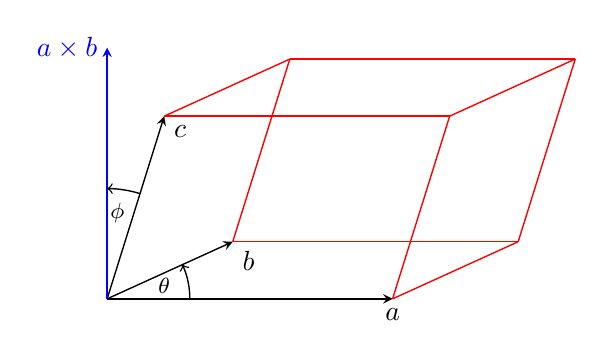
\begin{tikzpicture}[xscale=1.45, yscale=1.45]
    \coordinate (origin) at (0,0);
    \coordinate (z) at (1.1, 0.5);
    \coordinate (z1) at (2.5, 0);
    \coordinate (z2) at (0.5, 1.6);
    \coordinate (z3) at (0, 2.2);

    % \draw [->,>=stealth] (0, 0) -- (0, 1.75);
    \draw [->,>=stealth] (0, 0) -- (2.5, 0) node [anchor=north] {$\vv{a}$};
    \draw [->,>=stealth] (0, 0) -- (1.1, 0.5) node [anchor=north west] {$\vv{b}$};
    \draw [color=red] (2.5, 0) -- (3.6, 0.5);
    \draw [color=red] (1.1, 0.5) -- (3.6, 0.5);

    \draw [->,>=stealth] (0, 0) -- (0.5, 1.6) node [anchor=north west] {$\vv{c}$};
    \draw [color=red] (0.5, 1.6) -- (3.0, 1.6);
    \draw [color=red] (2.5, 0) -- (3.0, 1.6);

    \draw [color=red] (3.6, 0.5) -- (4.1, 2.1);
    \draw [color=red] (3.0, 1.6) -- (4.1, 2.1);

    \draw [color=red] (1.1, 0.5) -- (1.6, 2.1);
    \draw [color=red] (0.5, 1.6) -- (1.6, 2.1);

    \draw [color=red] (1.6, 2.1) -- (4.1, 2.1);

    \draw [->,>=stealth, color=blue] (0, 0) -- (0, 2.2) node [anchor=east] {$\vv{a} \times \vv{b}$};

    \pic [draw, ->, angle eccentricity=1.2, angle radius=1.05cm, color=black] {angle = z1--origin--z};
        
    \draw (0.5, 0.115) node {\footnotesize $\theta$};

    \pic [draw, ->, angle eccentricity=1.2, angle radius=1.4cm, color=black] {angle = z2--origin--z3};
        
    \draw (0.09, 0.75) node {\footnotesize $\phi$};
\end{tikzpicture}
\end{center}

In the sketch above (where we assume $\theta, \phi < \pi/2$), we have
$$
|\vv{c}| |\vv{a} \times \vv{b}| \cos \phi = \underbrace{|\vv{a}||\vv{b}| \sin \theta}_{\text{base area}} \cdot \underbrace{|\vv{c}| \cos \phi}_{\text{height}},
$$
which is the volume as shown. 

We do have a sign, and indeed we have that $\vv{c} \cdot (\vv{a} \times \vv{b}) > 0$ implies that $\vv{a},\vv{b}, \vv{c}$ is a right handed set. Also $\vv{c} \cdot (\vv{a} \times \vv{b}) = 0$ if and only if $\vv{a}, \vv{b}, \vv{c}$ are coplanar (corresponding with the parallelepiped having zero volume).

We can compute the scalar triple product using components. For $\vv{a} = (a_1, a_2, a_3)$, $\vv{b} = (b_1, b_2, b_3)$, $\vv{c} = (c_1, c_2, c_3)$, then we have
\begin{align*}
    \vv{a} \cdot (\vv{b} \times \vv{c}) &= a_1 b_2 c_3 - a_1 b_3 c_2 \\
    & + a_2 b_3 c_1 - a_2 b_1 c_3 \\
    & + a_3 b_1 c_2 - a_3 b_2 c_1 \\
    &= \begin{vmatrix}
        a_1 & a_2 & a_3 \\
        b_1 & b_2 & b_3 \\
        c_1 & c_2 & c_3 
    \end{vmatrix},
\end{align*}
which is a determinant (we shall study these in Section 5).

\subsubsection{Vector Triple Product}

Another slightly less used product on three vectors is the \emph{vector triple product}.

\begin{definition}[Vector Triple Product]
    For vectors $\vv{a}, \vv{b}, \vv{c}$, we define the \vocab{vector triple product} to be
    $$
    \vv{a} \times(\vv{b} \times \vv{c})=(\vv{a} \cdot \vv{c}) \vv{b}-(\vv{a} \cdot \vv{b}) \vv{c}.
    $$
\end{definition}

We will prove this identity later on, but note that this product is not associative. As the cross product is anticommutative, we do have
$$
\vv{a} \times(\vv{b} \times \vv{c}) = - (\vv{b} \times \vv{c}) \times \vv{a}.
$$

There's not really a sensible geometric interpretation of the vector triple product, but it is used in other vector formulas as it can shorten certain expressions.

\subsection{Lines, Planes \& Vector Equations}

We defined vectors as position vectors from an origin $O$, but with the introduction of vector addition, we can also use vectors to describe the displacement between two points,
$$
\vv{u} = \overrightarrow{QP} = \vv{p} - \vv{q}.
$$

\begin{center}
    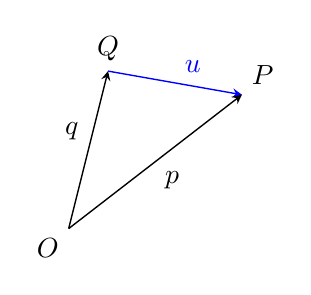
\begin{tikzpicture}
        \draw (0,0) node [anchor=north east] {$O$};
        \draw [->,>=stealth] (0,0) -- (0.5, 2) node [anchor=south] {$Q$} node [pos=0.5, anchor=south east] {$\vv{q}$};
        \draw [->,>=stealth, color=blue] (0.5,2) -- (2.2, 1.7) node [anchor=south west, color=black] {$P$} node [pos=0.5, anchor=south west] {$\vv{u}$};
        \draw [->,>=stealth] (0,0) -- (2.2, 1.7) node [pos=0.5, anchor=north west] {$\vv{p}$};
    \end{tikzpicture}
\end{center}

With this description of displacement vectors, we can define geometric objects such as lines and planes using equations involving vectors.

\subsubsection{Lines}

A general point on a line through $\vv{a}$ in the direction of $\vv{u} \neq \vv{0}$
can be written as
$$
\vv{r} = \vv{a} + \lambda \vv{u}, \quad \quad \lambda \in \R.
$$
This is known as the \vocab{parametric form} of the line. Note the similarity between this equation and the one for a line in the complex plane.

\begin{center}
    \begin{tikzpicture}
        \draw (0,0) node [anchor=north east] {$O$};

        \draw [dashed] (-1.5, 1.25) -- (3, 2.375);

        \draw [->,>=stealth] (0, 0) -- (-0.5, 1.5) node [anchor=north east] {$\vv{a}$};
        \draw [->, >=stealth] (-0.5, 1.5) -- (0.25, 1.6875) node [anchor=south] {$\vv{u}$};
        \draw [->, >=stealth, color=blue] (0,0) -- (2.25, 2.1875) node [anchor=north west] {$\vv{r}$};
    \end{tikzpicture}
\end{center}

To eliminate the parameter from this equation, we can take the cross product with $\vv{u}$
\begin{align*}
    \vv{u} \times \vv{r} &= \vv{u} \times (\vv{a} + \lambda \vv{u})\\
                         &= \vv{u} \times \vv{a}  \\
\implies \vv{u} \times (\vv{r} - \vv{a}) &= \vv{0}.
\end{align*}

With this in mind, consider also the related equation $\vv{u} \times \vv{r} = \vv{c}$ with $\vv{u}, \vv{c} \neq \vv{0}$. From this, $\vv{u} \cdot \vv{c} = \vv{u} \cdot (\vv{u} \times \vv{r}) = 0$, so if $\vv{u} \cdot \vv{c} \neq 0$, this is inconsistent and there are no solutions. Otherwise, if $\vv{u} \cdot \vv{c}= 0$, then $\vv{u} \times (\vv{u} \times \vv{c}) = -|\vv{u}|^2 \vv{c}$, so $\vv{a} = \frac{-1}{|\vv{u}|^2}(\vv{u} \times \vv{c})$ is one solution. Then $\vv{r} = \vv{a} + \lambda \vv{u}$ is the general solution.


\subsubsection{Planes}

A general point on a plane $\Pi$ through $\vv{a}$ with directions $\vv{u}, \vv{v}$ in the plane ($\vv{u} \not \parallel \vv{v}$) is
$$
\vv{r} = \vv{a} + \lambda \vv{u} + \mu \vv{v}, \quad \quad \lambda, \mu \in \R.
$$

\begin{center}
    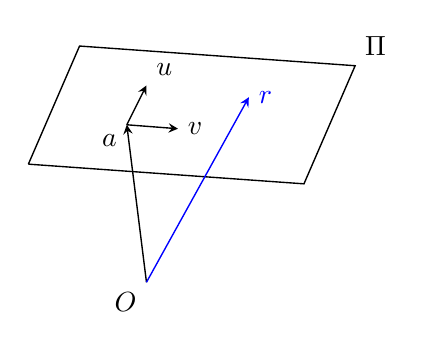
\begin{tikzpicture}
        \draw [color=black] (0, 0) -- (3.5, -0.25) -- (4.15, 1.25) -- (0.65, 1.5) -- (0,0);

        \draw (4.15, 1.25) node [color=black, anchor=south west] {$\Pi$};

        \draw (1.5,-1.5) node [anchor=north east] {$O$};

        % \draw [dashed] (-1.5, 1.25) -- (3, 2.375);

        
        \draw [->,>=stealth] (1.25, 0.5) -- (1.5, 1) node [anchor=south west] {$\vv{u}$};
        \draw [->,>=stealth] (1.25, 0.5) -- (1.9, 0.45) node [anchor=west] {$\vv{v}$};

        \draw [->,>=stealth] (1.5, -1.5) -- (1.25, 0.5) node [anchor=north east] {$\vv{a}$};

        \draw [->,>=stealth, color=blue] (1.5, -1.5) -- (2.8, 0.85) node [anchor=west] {$\vv{r}$};
    \end{tikzpicture}
\end{center}

An alternative form comes from considering a normal to the plane, $\vv{n}= \vv{u} \times \vv{v}$ ($\neq \vv{0}$). With this, we get
\begin{align*}
    \vv{n} \cdot \vv{r} &= \vv{n} \cdot \vv{a}  \\
\implies   \vv{n} \cdot (\vv{r} - \vv{a}) &= 0.
\end{align*}
For a geometric interpretation of this, note that $\vv{r} - \vv{a}$ is the displacement in the direction of the plane, and thus should be perpendicular to $\vv{n}$, a normal to the plane.

\subsubsection{Other Vector Equations}

To handle other vector equations, a general strategy is to manipulate equations and dot/cross with constant vectors.

\begin{example}[Vector Equation of a Sphere]
    We will attempt to find a geometric interpretation of the vector equation
    $$
    |\vv{r}|^2 + \vv{r} \cdot \vv{a} = k,
    $$
    with $\vv{a}$, $k$ constant.

    Here, we can `complete the square' to get
    $$
    \left|\vv{r} + \frac{1}{2}\vv{a}\right|^2 = k + \frac{1}{4}|\vv{a}|^2,
    $$
    which is a sphere with center $-\frac{1}{2}\vv{a}$ and radius $(k + \frac{1}{4}|\vv{a}|^2)^{1/2}$, if $k > - \frac{1}{4}|\vv{a}|^2$. If this is not the case, then there are no solutions.
\end{example}

\begin{example}[Arbitrary Vector Equation]
    We will solve the vector equation
    $$
    \vv{r} + \vv{a} \times (\vv{b} \times \vv{r}) = \vv{c},
    $$
    where $\vv{a}, \vv{b}, \vv{c}$ are given.

    We will use the `dot and cross stuff' approach. We use the vector triple product identity to rewrite this as
    \begin{equation}
        \vv{r} + (\vv{a} \cdot \vv{r}) \vv{b} - (\vv{a} \cdot \vv{b})\vv{r} = \vv{c} \tag{$\dagger$}.
    \end{equation}
    Then dotting with $\vv{a}$ we get
    \begin{align*}
        \vv{a} \cdot \vv{r} + (\vv{a} \cdot \vv{r})(\vv{b} \cdot \vv{a}) - (\vv{a} \cdot \vv{b})(\vv{a} \cdot \vv{r}) &= \vv{c} \cdot \vv{a} \nonumber \\
\implies \vv{a} \cdot \vv{r} &= \vv{c} \cdot \vv{a}. \tag{$\dagger \dagger$}
    \end{align*}
    Taking a dot product has `lost information', so we substitute $(\dagger \dagger)$ into $(\dagger)$ to get
    $$
    (1 - \vv{a} \cdot \vv{b}) \vv{r} = \vv{c} - (\vv{a} \cdot \vv{c}) \vv{b}.
    $$

    If $\vv{a} \cdot \vv{b} \neq 1$, then we can rearrange to get our solution
    $$
        \vv{r} = \frac{1}{1 - \vv{a} \cdot \vv{b}} ( \vv{c} - (\vv{a} \cdot \vv{c}) \vv{b}),
    $$
    which is a point.

    If $\vv{a} \cdot \vv{b} = 1$, then $\vv{c} - (\vv{a} \cdot \vv{c})\vv{b} \neq \vv{0}$ would cause the equation to be inconsistent. So if $\vv{c} - (\vv{a} \cdot \vv{c})\vv{b} = \vv{0}$, then $(\dagger)$ can be rewritten
    $$
    (\vv{a} \cdot \vv{r} - \vv{a} \cdot \vv{c}) \vv{b} = \vv{0},
    $$
    of which the set of solutions is given by $(\dagger \dagger)$, a plane.
\end{example}

\subsection{Index Notation \& The Summation Convention}

Returning to the component approach that we began to develop earlier, we will now introduce some machinery for working with components algebraically in a more streamlined way. The notation may look like mere bookkeeping at first, but it makes otherwise painful vector identities almost mechanical to prove.

\subsubsection{Components, $\delta$ and $\varepsilon$}

Begin by writing vectors $\vv{a}$, $\vv{b}$, $\dots$ in terms of components $a_i, b_i$ with respect to an orthonormal, right-handed basis $\{\vv{e}_i\}$. In the following discussion, the indices $i$, $j$, $k$, $l$, $p$, $q$, $\dots$ will take on values $1, 2, 3$\footnote{This corresponds to the number of basis vectors, and the approach used will naturally generalize to indices taking on more values.}.

Using indices, we can take some vector $\vv{c} = \alpha \vv{a} + \beta \vv{b}$ and express the components as $c_i = [\alpha \vv{a} + \beta \vv{b}]_i = \alpha a_i + \beta b_i$, for $i = 1, 2, 3$ (a \vocab{free variable}). Using the same notation, we can write things like
$$
\vv{a} \cdot \vv{b} = \sum_i a_i b_i,
$$
and
\begin{align*}
    \vv{x} &= \vv{a} + (\vv{b} \cdot \vv{c}) \vv{d} \\
\iff x_j &= a_j + \left(\sum_k b_k c_k\right) d_j, \quad \quad \text{for }j = 1, 2, 3.
\end{align*}

\begin{definition}[Kronecker Delta Symbol]
    We define the \vocab{Kronecker delta} symbol to be
    $$
    \delta_{ij} = \begin{cases}
        1 &\mbox{if } i = j, \\
        0 &\mbox{if } i \neq j.
       \end{cases}
    $$
\end{definition}

With this definition, we get $\vv{e}_i \cdot \vv{e}_j = \delta_{ij}$, which encodes our orthonormality condition from before. Then
\begin{align*}
    \vv{a} \cdot \vv{b} &= \left(\sum_i a_i \vv{e}_i\right)\cdot\left(\sum_j b_j \vv{e}_j\right) \\
    &= \sum_{ij} a_i b_j \vv{e}_i \cdot \vv{e}_j \\
    &= \sum_{ij} a_i b_j \delta_{ij} \\
    &= \sum_i a_i b_i.
\end{align*}

\begin{definition}[Levi-Civita Symbol]
    We define the \vocab{Levi-Civita symbol} such that
    $$
    \varepsilon_{ijk} = \begin{cases}
        +1 &\mbox{if } (i\ j\ k) \text{ is an even permutation of } (1\ 2\ 3), \\
        -1 &\mbox{if } (i\ j\ k) \text{ is an odd permutation of } (1\ 2\ 3), \\ 
        0 &\mbox{otherwise}
       \end{cases}
    $$
\end{definition}

For example,
\begin{align*}
    \varepsilon_{123} =  \varepsilon_{231} =  \varepsilon_{312} = +1, \\
    \varepsilon_{321} =  \varepsilon_{213} =  \varepsilon_{132} = -1, \\
    \varepsilon_{ijk} = 0 \text{ if any of } i,j,k \text{ repeat.}
\end{align*}

The Levi-Civita symbol is \vocab{totally antisymmetric}, in that exchanging a pair of indices produces a change in sign.

With this definition, in our right-handed orthonormal basis we have
$$
\vv{e}_i \times \vv{e}_j = \sum_k \varepsilon_{ijk} \vv{e}_k,
$$
for example
$$
\vv{e}_2 \times \vv{e}_1 = \sum_k \varepsilon_{21k}\vv{e}_k = \varepsilon_{213} \vv{e}_3 = - \vv{e}_3.
$$

So we can compute the cross product of two vectors as
\begin{align*}
    \vv{a}\times \vv{b} &= \left(\sum_i a_i \vv{e}_i\right) \times \left(\sum_j b_j \vv{e}_j\right) \\
    &= \sum_{ij} a_i b_j \vv{e}_i \times \vv{e}_j \\
    &= \sum_{ijk} a_i b_j \varepsilon_{ijk} \vv{e}_k \\
\iff (\vv{a} \times \vv{b})_k &= \sum_{ij} \varepsilon_{ijk} a_i b_j.
\end{align*}

For example, $(\vv{a} \times \vv{b})_3 = \sum_{ij} \varepsilon_{ij3} a_i b_j = \varepsilon_{123} a_1 b_2 + \varepsilon_{213} a_2 b_1 = a_1 b_2 - a_2 b_1$, as we had before.

\subsubsection{Summation Convention}

With components and index notation, indices that appear twice in a given term are usually summed over. In the \vocab{summation convention}, we omit the sigma ($\sum$) signs for repeated indices, and the sums are implicitly understood.

\begin{example}[Examples of the Summation Convention]
    The following all use the summation convention.
    \begin{enumerate}[label=(\roman*)]
        \item $a_i \delta_{ij} = a_1 \delta_{1j} + a_2 \delta_{2j} + a_3\delta_{3j} = a_j$.
        \item $\vv{a} \cdot \vv{b} = a_i b_i$.
        \item $(\vv{a} \times \vv{b})_i= \varepsilon_{ijk}a_j b_k$.
        \item $\vv{a} \cdot (\vv{b} \times \vv{c}) = \varepsilon_{ijk} a_i b_j c_k$.
        \item $\delta_{ii} = \delta_{11} + \delta_{22} + \delta_{33} = 3$.
        \item $[(\vv{a} \cdot \vv{c})\vv{b} - (\vv{a} \cdot \vv{b})\vv{c}]_i = (\vv{a} \cdot \vv{c})b_i - (\vv{a} \cdot \vv{b})c_i = a_j c_j b_i - a_k b_k c_i$.
    \end{enumerate}
\end{example}

We can explicitly define the rules of the summation convention as follows.

\begin{definition}[Summation Convention Rules]
    When using the summation convention, we have the following rules.
    \begin{enumerate}[label=(\roman*)]
        \item An index occurring exactly once in any given term must appear once in every term of an equation, and it can take any value -- a \vocab{free index}.
        \item Any index occurring exactly \emph{twice} in a given term is summed over -- a \vocab{repeated}, \vocab{contracted} or \vocab{dummy index}.
        \item No index can occur more than twice in a given term.
    \end{enumerate}
\end{definition}

Let's have a look at applying the summation convention to prove the vector triple product identity we stated earlier.

\begin{proposition}[Vector Triple Product Identity]
    For vectors $\vv{a}, \vv{b}, \vv{c}$, we have
    $$
    \vv{a} \times(\vv{b} \times \vv{c})=(\vv{a} \cdot \vv{c}) \vv{b}-(\vv{a} \cdot \vv{b}) \vv{c}.
    $$
\end{proposition}
\begin{proof}
We have
\begin{align*}
    [\vv{a} \times (\vv{b} \times \vv{c})]_i &= \varepsilon_{ijk} a_j (\vv{b} \times \vv{c})_k \\
        &= \varepsilon_{ijk} a_j \varepsilon_{kpq} b_p c_q \\
 &= (\varepsilon_{ijk}\varepsilon_{pqk}) a_j b_p c_q,
\end{align*}    
now $\varepsilon_{ijk}\varepsilon_{pqk} = \delta_{ip} \delta_{jq} - \delta_{iq} \delta_{jp}$ (we will prove this later on), hence
\begin{align*}
    [\vv{a} \times (\vv{b} \times \vv{c})]_i &= (\delta_{ip} \delta_{jq})a_j b_p c_q - (\delta_{iq} \delta_{jp}) a_j b_p c_q \\
    &= [(\vv{a} \cdot \vv{c})\vv{b} - (\vv{a} \cdot \vv{b})\vv{c}]_i,
\end{align*}
as required.
\end{proof}

\subsubsection{$\varepsilon \varepsilon$ Identities}

We will finish this section by looking at $\varepsilon \varepsilon$ identities, which can be used in various computations involving $\delta$ and $\varepsilon$ symbols.

\begin{itemize}
    \item $\varepsilon_{ijk}\varepsilon_{pqk} = \delta_{ip} \delta_{jq} - \delta_{iq} \delta_{jp} = \varepsilon_{kij} \varepsilon_{kpq}$.
    
    To check this, note that RHS and LHS are antisymmetric under $i \leftrightarrow j$, $p \leftrightarrow q$, so both vanish if $i$ \& $j$ or $p$ \& $q$ take the same value. Now it suffices to check examples $i = p = 1$, $j = q = 2$, where LHS and RHS are both $+1$, or $i = q = 1$, $j = p = 2$, where LHS and RHS are both $-1$. All other index choices giving non-zero results work similarly.

    \item $\varepsilon_{ijk} \varepsilon_{pjk} = 2 \delta_{ip}$.
    
    This comes from the above identity, where the LHS becomes $\delta_{ip} \delta_{jj} - \delta_{ij} \delta_{jp} = 3\delta_{ip} - \delta_{ip} = 2\delta_{ip}$.

    \item $\varepsilon_{ijk} \varepsilon_{ijk} = 6$.

    This follows directly from the previous result, with $i = p$. Then $2 \delta_{ii} = 6$.
\end{itemize}


\section{Vectors in a General Setting, $\R^n$ and $\C^n$}

In the previous chapter, we studied vectors as they occur when considering position vectors in three dimensions. However, vectors are more general objects, which we will see in this chapter. First, we will consider how to immediately generalise vectors from $\R^3$ (as in the previous chapter) to $\R^n$.

\subsection{Vectors in $\R^n$}

By regarding vectors as sets of components, it's easy to generalize from 3 to $n$ dimensions.

\begin{definition}[$\R^n$ Space]
    We define $\R^n$ to be the set of $n$-tuples of real numbers,
    $$
    \R^n = \{(x_1, x_2, \dots, x_n) \mid x_i \in \R\}.
    $$ 
    We also define \vocab{vector addition} and \vocab{scalar multiplication} as
    \begin{align*}
        (x_1, \dots, x_n) + (y_1, \dots, y_n) &= (x_1 + y_1, \dots, x_n + y_n),\\
       \text{and} \quad \lambda (x_1, \dots, x_n) &= (\lambda x_1, \dots, \lambda x_n).
    \end{align*}
\end{definition}

As before, we can take arbitrary linear combinations and we also get a notion of parallelism, where $\vv{x} \parallel \vv{y}$ if and only if $\vv{x} = \lambda \vv{y}$ or $\vv{y} = \lambda \vv{x}$ for $\lambda \in \R$.

We also still have a dot product, but in more general settings, such operations are normally referred to as \emph{inner products}.

\begin{definition}[Inner Product]
    The inner product on $\R^n$ is defined by
    $$
    \vv{x} \cdot \vv{y} = \sum_{i} x_i y_i = x_1 y_1 + x_2 y_2 + \cdots + x_n y_n.
    $$
\end{definition}

\begin{proposition}[Properties of the Inner Product]
    In $\R^n$, the inner product satisfies
    \begin{enumerate}[label=(\roman*)]
        \item \emph{Symmetric}. $\vv{x} \cdot \vv{y} = \vv{y} \cdot \vv{x}$.
        \item \emph{Bilinear}. $(\lambda \vv{x} + \lambda' \vv{x}') \cdot \vv{y} = \lambda \vv{x} \cdot \vv{y} + \lambda' \vv{x}' \cdot \vv{y}$.
        \item \emph{Positive Definite}. $\vv{x} \cdot \vv{x} = \sum_{i} x_i ^2 \geq 0$, and is equal 0 if and only if $\vv{x} = \vv{0}$. 
    \end{enumerate}
\end{proposition}

Also, if we return back to vectors in three-dimensions, we had an equivalent definition of the dot product as
$$
\vv{x} \cdot \vv{y} = |\vv{x}| |\vv{y}| \cos \theta,
$$
where $\theta$ is the angle between the vectors. Using this as a definition of the inner product in $\R^n$, we get a definition for the angle between vectors.

When we look at vector spaces in general, we will define the inner product in general to be any operation that satisfies these properties.

We also have the notions of length and orthogonality, much the same as in three-dimensions.

\begin{definition}[Length/Norm]
    For $\vv{x} \in \R^n$, we define its \vocab{length} or \vocab{norm} to be $|\vv{x}| \geq 0$ with $|\vv{x}|^2 = \vv{x} \cdot \vv{x}$.
\end{definition}

\begin{definition}[Orthogonality]
    We say two vectors $\vv{x}, \vv{y} \in \R^n$ are \vocab{orthogonal} if and only if $\vv{x} \cdot \vv{y} = 0$.
\end{definition}

When working in $\R^n$, we typically use a set of basis vectors known as the \vocab{standard basis}. They are
\begin{align*}
    \vv{e}_1 &= (1, 0, 0, \dots, 0), \\
    \vv{e}_2 &= (0, 1, 0, \dots, 0), \\
        &\vdots \\
        \vv{e}_n &= (0, 0, 0, \dots, 1).
\end{align*}
Then we have
$$
\vv{x} = \sum_i x_i \vv{e}_i,
$$
and $\vv{e}_i \cdot \vv{e}_j = \delta_{ij}$, so this basis is orthonormal.

\subsubsection{Cauchy-Schwarz and the Triangle Inequality}

We will now state an inequality about the inner product of two vectors in $\R^n$.

\begin{proposition}[Cauchy-Schwarz Inequality]
    For all vectors $\vv{x}, \vv{y} \in \R^n$, we have
    $$
|\vv{x} \cdot \vv{y}| \leq |\vv{x} | \cdot |\vv{y}|,
    $$
    with equality if and only if $\vv{x} \parallel \vv{y}$.
\end{proposition}
\begin{proof}
    If $\vv{y} = \vv{0}$, then we are done. Otherwise, consider
    \begin{align*}
        |\vv{x} - \lambda \vv{y}|^2 &= (\vv{x} - \lambda\vv{y}) \cdot (\vv{x} - \lambda \vv{y}) \\
        &= |\vv{x}|^2 - 2 \lambda \vv{x} \cdot \vv{y} + \lambda^2 |\vv{y}|^2 \geq 0
    \end{align*}
    for any $\lambda \in \R$. This is a real quadratic in $\lambda$ with at most one real root, so its discriminant satisfies
    $$
    (-2 \vv{x} \cdot \vv{y})
^2 - 4|\vv{x}|^2 |\vv{y}|^2 \leq 0,    $$
which rearranges to give $|\vv{x} \cdot \vv{y}| \leq |\vv{x}||\vv{y}|$. Equality holds if and only if the discriminant is zero, that is, if $\vv{x} = \lambda \vv{y}$ for some $\lambda$, as required.
\end{proof}

As vectors in $\R^n$ are just sets of components, we can state this inequality in terms of real numbers.
    For sequences of real numbers $(a_i)$ and $(b_i)$, we have
    $$
\left(\sum_{i = 1}^n a_i b_i\right)^2 \leq \left(\sum_{i = 1}^n a_i^2 \right)\left(\sum_{i = 1}^n b_i^2 \right),
    $$
    where we have equality if and only if $\frac{a_i}{b_i}$ is a constant for all $i$ where $a_i b_i \neq 0$.

We also have the triangle inequality, similar to the one stated in Section 1.

\begin{proposition}[Triangle Inequality]
    For all $\vv{x},\vv{y} \in \R^n$,
    $$
    |\vv{x} + \vv{y} |\leq |\vv{x}| + |\vv{y}|
    $$
\end{proposition}
\begin{proof}
We have
\begin{align*}
    |\vv x + \vv y|^2 &= |\vv x|^2 + 2 \vv{x}\cdot \vv{y} + |\vv{y}|^2 \\
    &\leq |\vv{x}|^2 + 2 |\vv{x}| \cdot |\vv{y}| + |\vv{y}|^2 \\
    &= (|\vv{x}| + |\vv{y}|)^2,
\end{align*}
as required.
\end{proof}

\subsubsection{A comment about $\R^n$ and $\R^3$}

The definition we gave for the inner product on $\R^n$ can be written as
$$
\vv{a} \cdot \vv{b} = \delta_{ij} a_i b_j,
$$
for $\vv{a}, \vv{b} \in \R^n$ where we use the summation convention. For $n = 3$, this matches with the compact definition of the dot product we gave previously.

However, in three dimensions we also had a compact definition of the cross product with
$$
(\vv{a} \times \vv{b})_i = \varepsilon_{ijk} a_j b_k.
$$
In $\R^n$ however, we have $\varepsilon_{ij\dots k}$ where there are $n$ indices (we will look at this again in Section 5). This is totally antisymmetric, so we cannot use $\varepsilon$ to define a vector-valued product for any $n$ except $3$. 

In $\R^2$ however, we have $\varepsilon_{ij}$ where $\varepsilon_{12} = - \varepsilon_{21} = 1$, and we can define an additional scalar product
$$
[\vv{a}, \vv{b}] = \varepsilon_{ij}a_i b_j = a_1 b_2 - a_2 b_1.
$$
This corresponds with the signed area of a parallelogram, and $|[\vv{a}, \vv{b}]| = |\vv{a}| |\vv{b}| \sin \theta$. Compare this with $[\vv{a}, \vv{b}, \vv{c}] = \varepsilon_{ijk}a_i b_j c_k$, the signed volume of the parallelepiped in three dimensions we defined earlier.

\subsection{Vector Spaces}

We will now go one step further and define what a vector is in a much more general sense.
This will be done by defining the properties that vectors have, rather than what they are themselves.

\begin{definition}[Vector Space]
  Let $V$ be a set of objects called \vocab{vectors} with operations $\vv{v} + \vv{w} \in V$ defined for all $\vv{v}, 
\vv{w} \in V$, and $\lambda \vv{v} \in V$ for all $\vv{v} \in V$ and $\lambda \in F$, where $F$ is some field. 

Then $V$ is a \vocab{vector space} if
\begin{enumerate}[label=(\roman*)]
    \item $V$ with $+$ is an abelian group.
    \item $\lambda( \vv{v} + \vv{w}) = \lambda \vv{v} + \lambda \vv{w}$.
    \item $(\lambda  + \mu)\vv{v} = \lambda \vv{v} + \mu \vv{v}$.
    \item $\lambda (\mu \vv{v}) = (\lambda \mu) \vv{v}$.
    \item $1 \vv{v} = \vv{v}$.
\end{enumerate}
\end{definition}

In this course, we will deal only with the fields $\R$ and $\C$. If $F = \R$, then we call $V$ a \vocab{real vector space}, and if $F = \C$, then we call it a \vocab{complex vector space}.

\begin{example}[Example of a Real Vector Space]
  Let $V$ be the set of all functions $f: [0, 1] \rightarrow \R$ where $f(0) = f(1) = 0$ and $f$ is smooth. Then $V$ is a real vector space.

  Indeed we have
  \begin{align*}
      (f + g)(x) &= f(x) + g(x), \\
      (\lambda f)(x) &= \lambda (f(x)).
  \end{align*}
  The other properties can be checked as required.
\end{example}

We can also define a \emph{subspace} in the natural way.

\begin{definition}[Subspace]
    A \vocab{subspace} of a vector space $V$ is a subset $U \subseteq V$ that is also a vector space.
\end{definition}

Note that a non-empty subset is a subspace if and only if $\vv{v}, \vv{w} \in U$ implies $\lambda \vv{v} + \mu \vv{w} \in U$ where $\lambda, \mu$ are some arbitrary scalars.

For any vectors $\vv{v}_1, \vv{v}_2, \dots, \vv{v}_r \in V$, their span
$$
    \vecspan \{\vv{v}_1, \dots, \vv{v}_r\} = \{ \lambda_1 \vv{v}_1 + \cdots + \lambda_r \vv{v}_r \mid \lambda_i \in \R \text{ or } \C \}.
$$
is a subspace. Also note that $V$ and $\{ \vv{0} \}$ are both subspaces of a vector space $V$.

\subsubsection{Linear Dependence \& Independence}

We will now think about whether sets of vectors are independent. 

\begin{definition}[Linear Dependence/Independence]
    For $\vv{v}_1, \vv{v}_2, \dots, \vv{v}_r \in V$, some vector space, consider the \vocab{linear relation}
    \begin{equation}\label{eq:dag}
        \lambda_1 \vv{v}_1 + \lambda_2 \vv{v}_2 + \cdots + \lambda_r \vv{v}_r = \vv{0} \tag{$\dagger$}
    \end{equation}
    If \eqref{eq:dag} implies that $\lambda_i = 0$ for all $i$, then these vectors form a \vocab{linearly independent} set. If \eqref{eq:dag} holds with some $\lambda_i \neq 0$, then they form a \vocab{linearly dependent} set.
\end{definition}


\begin{example}[Example of a Linearly Dependent Set]
    In $\R^2$, the set $\left\{\begin{pmatrix}1 \\ 0\end{pmatrix}, \begin{pmatrix}0 \\ 1\end{pmatrix}, \begin{pmatrix}0 \\ 2\end{pmatrix}\right\}$ is linearly dependent, since
    $$
    0\begin{pmatrix}1 \\ 0\end{pmatrix} + 2\begin{pmatrix}0 \\ 1\end{pmatrix} - 1\begin{pmatrix}0 \\ 2\end{pmatrix} = \begin{pmatrix}0 \\ 0\end{pmatrix},
    $$
    which is a non-trivial linear relation.
\end{example}

Any set containing $\vv{0}$ is linearly dependent, since $\lambda \vv{0} = \vv{0}$ for any $\lambda \neq 0$.

In $\R^3$, the set of vectors $\{\vv{a}, \vv{b}, \vv{c}\}$ are linearly independent if $\vv{a} \cdot (\vv{b} \times \vv{c}) \neq 0$, since if $\alpha \vv{a} + \beta \vv{b} + \gamma \vv{c} = \vv{0}$, then dotting with $\vv{b} \times \vv{c}$ gives $\alpha \vv{a} \cdot (\vv{b} \times \vv{c}) = 0 \implies \alpha = 0$, and $\beta, \gamma$ similarly.


\subsubsection{Inner Products}

A real vector space can have an additional structure that we can define by axioms.

\begin{definition}[Inner Product]
    For a real vector space $V$ and $\vv{v}, \vv{w} \in V$, an \vocab{inner product} denoted by
    $$
    \vv{v} \cdot \vv{w} \quad \text{or} \quad (\vv{v}, \vv{w}) \in \R
    $$
    is a map that is symmetric, bilinear, and positive definite.
\end{definition}

If these conditions hold, then we get things like the Cauchy-Schwarz inequality and a norm as by the previous argument.

\begin{example}[Inner Product on a Real Vector Space]
    Consider the real vector space of functions $V = \{ f: [0, 1] \rightarrow \R \mid f \text{ smooth, and } f(0) = f(1) = 0 \}$.
    We can define the inner product as
    $$
    (f, g) = \int_0^1 f(x)g(x) \; \mathrm{d}x,
    $$
    which satisfies the conditions specified above. Then we have
    $$
    |(f, g)| \leq \norm{f} \cdot \norm{g},
    $$
    that is,
    $$
    \left| \int_0^1 f(x)g(x)\; \mathrm{d}x \right| \leq \left(\int_0^1 f(x)^2\; \mathrm{d}x\right)^{1/2} \left(\int_0^1 g(x)^2\; \mathrm{d}x\right)^{1/2}.
    $$
\end{example}

We can also say something about linear independence from an inner product.

\begin{lemma}
In any real vector space $V$ with an inner product, if $\vv{v}_1, \vv{v}_2, \dots, \vv{v}_r$ are non-zero and orthogonal vectors, then they are linearly independent.
\end{lemma}
\begin{proof}
    If $\sum_i \alpha_i \vv{v}_i = \vv{0}$, then $(\vv{v}_j, \sum_i \alpha_i \vv{v}_i) = 0$ for a fixed $j$, so $\alpha_j (\vv{v}_j, \vv{v}_j) = 0$, and thus $\alpha_j = 0$.
\end{proof}

\subsection{Basis and Dimension}

We can generalize the notion of a basis to an arbitrary vector space.

\begin{definition}[Basis]
    For a vector space $V$, a \vocab{basis} is a set $B = \{\vv{e}_1, \vv{e}_2, \dots, \vv{e}_n \}$ such that
    \begin{enumerate}[label=(\roman*)]
        \item $B$ spans $V$, that is, any $\vv{v} \in V$ can be written $\vv{v} = \sum_{i = 1}^n v_i \vv{e}_i$.
        \item $B$ is linearly independent.
    \end{enumerate}
\end{definition}

The linear independence implies that the coefficients $v_i$ in (i) are unique. We say that $v_i$ are the components of $\vv{v}$ with respect to the basis $B$.

\begin{example}[Standard Basis]
    The standard basis for $\R^n$ consists of the vectors
    $$
\vv{e}_1 = \begin{pmatrix}1 \\ 0\\ \vdots \\ 0\end{pmatrix}, \quad \vv{e}_2 = \begin{pmatrix}0 \\ 1\\ \vdots \\ 0\end{pmatrix}, \quad \dots, \quad \vv{e}_n = \begin{pmatrix}0 \\ 0\\ \vdots \\ 1\end{pmatrix}.
    $$
    This is a basis since it satisfies the definition as $\vv{x} \in \R^n$, we have
    $$
\vv{x} = \begin{pmatrix}x_1 \\ x_2\\ \vdots \\ x_n\end{pmatrix} = x_1 \vv{e}_1 + \cdots + x_n \vv{e}_n,
    $$
    and $\vv{x} = \vv{0}$ if and only if $x_1 = x_2 = \cdots = x_n = 0$. 
\end{example}

Of course in the example above we just used one particular base. 
For example in $\R^2$ another basis consists of $\{(1, 0), (1, 1)\}$. 

\begin{theorem}[The Basis Theorem]
    If $\{\vv{e}_1, \dots, \vv{e}_n\}$ and $\{\vv{f}_1, \dots, \vv{f}_m\}$ are both bases of a vector space $V$, then $n = m$.
\end{theorem}
\begin{proof}
    We can find coefficients $A_{ai}$ and $B_{ia}$ such that $\vv{f}_a = \sum_i A_{ai} \vv{e}_i$ and $\vv{e}_i = \sum_a B_{ia} \vv{f}_a$. So we have that
    \begin{align*}
    \vv{f}_a &= \sum_i A_{ai} \left(\sum_b B_{ib} \vv{f}_b\right) \\
        &= \sum_b \left(\sum_{i} A_{ai} B_{ib}\right)\vv{f}_b,
\end{align*}
    but coefficients with respect to a basis are unique, hence
    $$
    \sum_{i} A_{ai} B_{ib} = \delta_{ab}.
    $$
    Similarly, $\sum_{a} B_{ia} A_{aj} = \delta_{ij}$. Finally,
    \begin{align*}
        \sum_{ia} A_{ai} B_{ia} &= \sum_{a} \delta_{aa} = m \\
        &= \sum_i \delta_{ii} = n,
     \end{align*}
     hence $n = m$.
\end{proof}

This theorem allows us to state the following definition.

\begin{definition}[Dimension]
    The \vocab{dimension} of a vector space $V$, written $\operatorname{dim} V$, is the size of its basis.
\end{definition}

Note that $\R^n$ has dimension $n$.

The steps in the proof of the basis theorem are within the scope of the course, but you will not be expected to prove this theorem without prompts (it is non-examinable in the schedules). The same applies with the following.


\begin{proposition}
    Let $V$ be a vector space with finite subsets $Y = \{\vv{w}_1, \vv{w}_2, \dots, \vv{w}_m\}$ that spans $V$, and $X = \{\vv{u}_1, \dots, \vv{u}_k \}$ that is linearly independent. Then $k \leq n \leq m$ where $n = \operatorname{dim} V$. Also
    \begin{enumerate}[label=(\roman*)]
        \item A basis can be formed from subsets of $Y$,
        \item A basis can be obtained from $X$ by adding additional vectors (from $Y$ if necessary).
    \end{enumerate}
\end{proposition}
\begin{proof}
    \begin{enumerate}[label=(\roman*)]
        \item If $Y$ is linearly independent, then it's a basis and $m = n = \operatorname{dim} V$. If $Y$ is not linearly independent, then
        $$
        \sum_{i = 1}^m \lambda_i \vv{w}_i = \vv{0}, \quad \text{with some } \lambda_i \neq 0.
        $$
        Take $\lambda_m \neq 0$ without loss of generality, then $\vv{w}_m = -\frac{1}{\lambda_m} \sum_{i = 1}^{m - 1} \lambda_i \vv{w}_i$,
        so $\vecspan Y = \vecspan Y'$, with $Y' = \{\vv{w}_1, \dots, \vv{w}_{m - 1}\}$. This can be repeated until a basis is obtained.
        \item If $X$ spans $V$ then it's a basis and $k = n = \operatorname{dim} V$. If not, then there exists $\vv{u}_{k + 1} \in V$ not in $\vecspan X$. But then $\sum_{i = 1}^{k + 1} \mu_i \vv{u}_i = \vv{0}$ implies $\mu_{k + 1} = 0$, thus $X' = \{\vv{u}_1, \dots, \vv{u}_{k + 1} \}$ is linearly independent. Furthermore, we can choose $\vv{u}_{k + 1} \in Y$ as otherwise $Y \subseteq \vecspan X \implies \vecspan Y \subseteq \vecspan X \implies \vecspan X = V$.
        We can repeat this process until we obtain a basis (and this must stop since $Y$ is a finite set).   \qedhere
    \end{enumerate}
\end{proof}

Not every vector space has a finite dimension, but in this course we will deal only with vector spaces that do, save for the occasional example.

\begin{example}[Example of an Infinite Dimensional Vector Space]
    Consider the vector space
    $$
    V = \{ f : [0, 1] \rightarrow \R \mid \text{f smooth, } f(0) = f(1) = 0 \}. 
    $$
    Then consider $S_n(x) = \sqrt{2} \sin(n \pi x)$, $n = 1, 2, \dots$. These belong to $V$ and
    $$
    (S_n, S_m) = 2 \int_{0}^1 \sin (n \pi x) \sin (m \pi x) \; \mathrm{d}x = \delta_{mn},
    $$
    so they are all linearly independent. But we have infinitely many of them, so $V$ is infinite dimensional.
\end{example}

\subsection{Vectors in $\C^n$}

So far we have looked at real vector spaces, and particularly at $\R^n$. We can define a similar vector space over the complex numbers.

\begin{definition}[$\C^n$ Space]
    We define $\C^n$ to be the set of $n$-tuples of complex numbers,
    $$
    \C^n = \{(z_1, z_2, \dots, z_n) \mid z_j \in \C\}.
    $$
    We also define \vocab{addition} and scalar multiplication with
    \begin{align*}
        \left(z_{1}, \ldots, z_{n}\right)+\left(w_{1}, \ldots, w_{n}\right)&=\left(z_{1}+w_{1}, \ldots, z_{n}+w_{n}\right) \\
        \text{and} \quad \lambda\left(z_{1}, \ldots, z_{n}\right)=\left(\lambda z_{1}, \ldots, \lambda z_{n}\right) 
    \end{align*}
\end{definition}

Note that we could have used real scalars and have gotten a real vector space, but having a complex vector space is more natural. 

The distinction between real and complex vector spaces is important. For example, if we have $\vv{z} = (z_1, \dots, z_n) \in \C^n$, with $z_j = x_j + i y_j$ then
$$
\vv{z} = \sum_j x_j \vv{e}_j + \sum_j y_j \vv{f}_j, \quad \text{where } \vv{f}_j = i \vv{e}_j,
$$
is a real linear combination, and thus $\{\vv{e}_1, \dots, \vv{e}_n, \vv{f}_1, \dots, \vv{f}_n\}$ is a basis for $\C^n$ as a real vector space, and it has dimension $2n$. However, taking $\C^n$ as defined before, it is of dimension $n$ which is clearly different.

From now on we will view $\C^n$ as a complex vector space unless we say otherwise.

\subsubsection{Complex Inner Product}

We can define an inner product on $\C^n$.

\begin{definition}[Complex Inner Product]
    For $\vv{z}, \vv{w} \in \C^n$, we define the inner product to be
    $$
    (\vv{z}, \vv{w}) = \sum_j \overline{z_j} w_j = \overline{z_1} w_1 + \cdots + \overline{z_n} w_n.
    $$
\end{definition}

\begin{proposition}[Properties of the Complex Inner Product]
    The complex inner product satisfies
    \begin{enumerate}[label=(\roman*)]
        \item \emph{Hermitian}. $(\vv{w}, \vv{z}) = \overline{(\vv{z}, \vv{w})}$.
        \item \emph{Linear/anti-linear}. $(\vv{z}, \lambda \vv{w}+ \lambda' \vv{w}') = \lambda(\vv{z}, \vv{w}) + \lambda' (\vv{z}, \vv{w}')$ and $(\lambda \vv{z} + \lambda' \vv{z}', \vv{w}) = \overline{\lambda}(\vv{z}, \vv{w}) + \overline{\lambda'} (\vv{z}' , \vv{w})$.
        \item \emph{Positive definite}. $(\vv{z}, \vv{z}) = \sum_j |z_j|^2$, which is real, non-negative and zero if and only if $\vv{z} = \vv{0}$.
    \end{enumerate}
\end{proposition}
\begin{proof}[Proof Sketch]
    Check definitions.
\end{proof}

We also define the \emph{length} or \emph{norm} of $\vv{z}$ to be $|\vv{z}| \geq 0$ with $|\vv{z}|^2 = (\vv{z}, \vv{z})$.

We can also say that $\vv{z}, \vv{w} \in \C^n$ are orthogonal if $(\vv{z}, \vv{w}) = 0$. With this, note that the standard basis for $\C^n$ is orthonormal.

\section{Matrices and Linear Maps}

Vector spaces have two basic operations: addition and scalar multiplication. 
The prominence of these operations makes thinking about functions that preserve this structure quite useful. Such functions are called linear maps, and in the setting of finite dimensional vector spaces we have a useful way of studying them: matrices. In this chapter we will study both ideas and how they link together.

\subsection{Linear Maps}

Let's begin by defining what we mean exactly by a linear map.

\begin{definition}[Linear Map]
    A \vocab{linear map} or \vocab{linear transformation} is a function $T : V \rightarrow W$ between two vector spaces $V$ and $W$ such that
    $$
    T(\lambda \vv{x} + \mu \vv{y}) = \lambda T(\vv{x}) + \mu T(\vv{y}),
    $$
    for all $\vv{x}, \vv{y} \in V$ and $\lambda, \mu \in \R$ or $\C$\footnote{Depending on whether we are working with real or complex vector spaces.}.
\end{definition}

From this definition, it is immediately clear that a linear map is completely determined by its action on a set of basis vectors.

Let's have a look at some examples of linear maps that appear in geometry.

\begin{example}[Geometric Linear Maps]
The following are all examples of linear maps.
\begin{enumerate}[label=(\roman*)]
    \item A rotation is an example of a linear map. In $\R^2$, a rotation about $\vv{0}$ through an angle $\theta$ is defined by
    \begin{align*}
        \vv{e}_1 \mapsto \vv{e}_1' &= \cos \theta \, \vv{e}_1 + \sin \theta \, \vv{e}_2 \\
        \vv{e}_2 \mapsto \vv{e}_2' &= -\sin \theta \, \vv{e}_1 + \cos \theta \, \vv{e}_2
    \end{align*}
    
    \begin{center}
        \begin{tikzpicture}
            % angle 40 degrees
          \draw [->] (0, 0) -- (2.75, 0) node [right] {$\vv{e}_1$};
          \draw [->] (0, 0) -- (0, 2.75) node [above] {$\vv{e}_2$};
          \draw [->, color=blue] (0, 0) -- (2.107, 1.768) node [anchor=south west] {$\vv{e}_1'$} node [pos=0.3, below] {$\theta$};
          \draw [->, color=blue] (0, 0) -- (-1.768, 2.107) node [anchor=south east] {$\vv{e}_2'$};
        %   \draw [dashed] (0, 1.7) node [left] {$y$} -- (2.5, 1.7) -- (2.5, 0) node [below] {$x$};
        \end{tikzpicture}
      \end{center}
    
      In $\R^3$, a rotation about an axis given by $\vv{e}_3$ is defined as above, but with $\vv{e}_3 \mapsto \vv{e}_3'= \vv{e}_3$.

      \item A projection onto a plane through the origin with unit normal $\hat{\vv{n}}$ is a linear map, defined by
      $$
      \vv{x} \mapsto \vv{x}'= \vv{x}_{\perp} = \vv{x} - (\vv{x} \cdot \hat{\vv{n}}) \hat{\vv{n}}.
        $$
        Similarly, the reflection about that plane is a linear map, defined by
        $$
        \vv{x} \mapsto \vv{x}' = \vv{x} - 2(\vv{x} \cdot \hat{\vv{n}}) \hat{\vv{n}}
        $$
    \item A dilation along the basis vectors with scale factors $\alpha, \beta, \gamma$ is a linear map, defined by
    $$
    \vv{e}_1 \mapsto \vv{e}_1' = \alpha \vv{e}_1, \quad \vv{e}_2 \mapsto \vv{e}_2' = \beta \vv{e}_2, \quad \vv{e}_3 \mapsto \vv{e}_3' = \gamma \vv{e}_3.
    $$
    \item For orthogonal unit vectors $\vv{a}, \vv{b} \in \R^3$ and $\lambda \in \R$, we can define a \emph{shear} to be the linear map
    $$
      \vv{x} \mapsto \vv{x}' = \vv{x} + \lambda \vv{a} (\vv{x} \cdot \vv{b}).
    $$
    This displaces each point in the direction of $\vv{a}$, by an amount proportional to how far along $\vv{b}$ the point lies.
\end{enumerate}
\end{example}

When we have a linear map $T: V \rightarrow W$, it can be helpful to think about what vectors in the vector space $W$ are in the image of this function, and also what in $V$ will just be sent to $\vv{0}$. Because we deal with these so commonly, we introduce standard terms.

\begin{definition}[Image and Kernel]
    If $T: V \rightarrow W$ is a linear map, we say that its \vocab{image} is the set
    $$
    \img(T) = \{ \vv{x}' \in W \mid \vv{x}' = T(\vv{x}) \text{ for some } \vv{x} \in V\},
    $$ 
    and its \vocab{kernel} is the set
    $$
    \ker (T) = \{ \vv{x} \in V \mid T(\vv{x}) = \vv{0}\}.
    $$
\end{definition}

\begin{proposition}[Image and Kernel are Subspaces]
    If $T : V \rightarrow W$ is a linear map, then $\ker(T)$ is a subspace of $V$ and $\img(T)$ is a subspace of $W$.
\end{proposition}
\begin{proof}[Proof Sketch]
    Use the properties of $T$ as a linear map to check definitions.
\end{proof}

These subspaces have a special property relating to their dimension.
We call the dimension of the image the \vocab{rank} and dimension of the kernel as the \vocab{nullity} of a linear map. Then we have the following result (the proof of which is non-examinable).

\begin{theorem}[Rank-Nullity Theorem]
    For a linear map $T: V \rightarrow W$, we have $\rank(T) + \nullity(T) = \dim V$.
\end{theorem}
\begin{proof}
    Let $\vv{e}_1, \dots, \vv{e}_k$ be a basis for $\ker (T)$. Extend this by adding in $\vv{e}_{k + 1}, \dots, \vv{e}_n$ to get a basis for $V$. We claim that $B = \{T(\vv{e_{k + 1}}), \dots, T(\vv{e}_n)\}$ is a basis for $\img (T)$ (from which the result would follow).

    First we have that $B$ spans $\img(T)$, since for any $\vv{x} = \sum_{i =1}^n x_i \vv{e}_i \in V$, $T(\vv{x}) = \sum_{i = k+1}^n x_i T(\vv{e}_i)$. Also, $B$ is linearly independent since $\sum_{i = k + 1}^n \lambda_i T(e_i) = \vv{0}$ implies that $T\left(\sum_{i = k + 1}^n \lambda_i \vv{e}_i\right) = \vv{0}$. But then that linear combination must be in the kernel, so we must have $\lambda_i = 0$, as $\{\vv{e}_1, \dots, \vv{e}_n\}$ are linearly independent. Thus $B$ is a basis, as required.
\end{proof}


\subsection{Matrices}

In the examples above, we described linear maps by giving their action on basis vectors, or by giving an explicit formula for the image of a general vector $\vv{x}$. We are now going to introduce \emph{matrices}, which give us a uniform (and highly computable) way of doing this.

Let $T : \R^n \rightarrow \R^m$ be a linear map, and write $\vv{x}' = T(\vv{x})$.
Taking the standard basis $\{\vv{e}_1, \dots, \vv{e}_n\}$ of $\R^n$, we can write any $\vv{x} \in \R^n$ as $\vv{x} = \sum_j x_j \vv{e}_j$. Then by linearity,
$$
\vv{x}' = T\left(\sum_j x_j \vv{e}_j\right) = \sum_j x_j T(\vv{e}_j),
$$
so taking components in $\R^m$,
$$
x_i' = \sum_j [T(\vv{e}_j)]_i \, x_j.
$$
This motivates the following definition.

\begin{definition}[Matrix of a Linear Map]
	Let $T: \R^n \rightarrow \R^m$ be a linear map. The \vocab{matrix} of $T$ (with respect to the standard bases) is the $m \times n$ array of numbers $A = \{A_{ij}\}$ with entries
	$$
	A_{ij} = [T(\vv{e}_j)]_i,
	$$
	that is, the $j$th column of $A$ is the image of the $j$th basis vector. We write
	$$
	A = \begin{pmatrix}
		A_{11} & \cdots & A_{1n} \\
		\vdots & \ddots & \vdots \\
		A_{m1} & \cdots & A_{mn}
	\end{pmatrix},
	$$
	where $A_{ij}$ is the entry in row $i$ and column $j$, and we define the action of $A$ on a vector by $\vv{x}' = A \vv{x}$ where $x_i' = \sum_{j} A_{ij} x_j$, or with the summation convention just $x_i' = A_{ij}x_j$.
\end{definition}

The fact that \emph{the columns of the matrix are the images of the basis vectors} is worth internalising -- it is how one actually writes down matrices in practice, and we will use it constantly. The same definitions work with $\C^n$ and $\C^m$ (or indeed between any vector spaces with a choice of basis, as we will see when changing bases in Section 7).

Let's use this to write down matrices for the geometric linear maps we met before, working in $\R^2$ and $\R^3$.

\begin{example}[Matrices of Geometric Maps]
	\begin{enumerate}[label=(\roman*)]
		\item A rotation about $\vv{0}$ through angle $\theta$ in $\R^2$ sends $\vv{e}_1 \mapsto \cos \theta \, \vv{e}_1 + \sin \theta\, \vv{e}_2$ and $\vv{e}_2 \mapsto -\sin \theta \,\vv{e}_1 + \cos \theta\, \vv{e}_2$. Putting these images in as columns, the matrix of the rotation is
		$$
		R(\theta) = \begin{pmatrix}
			\cos \theta & - \sin \theta \\
			\sin \theta & \cos \theta
		\end{pmatrix}.
		$$
		In $\R^3$, a rotation by $\theta$ about the $\vv{e}_3$ axis fixes $\vv{e}_3$, giving
		$$
		R = \begin{pmatrix}
			\cos \theta & - \sin \theta & 0\\
			\sin \theta & \cos \theta & 0 \\
			0 & 0 & 1
		\end{pmatrix}.
		$$
		\item A reflection in the plane through the origin with unit normal $\hat{\vv{n}}$ is $\vv{x} \mapsto \vv{x} - 2 (\vv{x} \cdot \hat{\vv{n}}) \hat{\vv{n}}$, which in components reads $x_i' = x_i - 2 x_j n_j n_i$. So the matrix has entries
		$$
		H_{ij} = \delta_{ij} - 2 n_i n_j.
		$$
		\item A dilation with scale factors $\alpha, \beta, \gamma$ along the coordinate axes has matrix
		$$
		\begin{pmatrix}
			\alpha & 0 & 0 \\
			0 & \beta & 0 \\
			0 & 0 & \gamma
		\end{pmatrix}.
		$$
		\item The shear $\vv{x} \mapsto \vv{x} + \lambda \vv{a}(\vv{x} \cdot \vv{b})$ with $\vv{a} = \vv{e}_1$, $\vv{b} = \vv{e}_2$ has matrix
		$$
		S_\lambda = \begin{pmatrix}
			1 & \lambda & 0 \\
			0 & 1 & 0 \\
			0 & 0 & 1
		\end{pmatrix},
		$$
		which displaces points in the $\vv{e}_1$ direction by an amount proportional to their $\vv{e}_2$ component.
	\end{enumerate}
\end{example}

It's also worth knowing what a rotation about a \emph{general} axis looks like, and index notation makes the derivation quite pleasant.

\begin{proposition}[Rotation About a General Axis]
	Let $R$ be the rotation through angle $\theta$ about an axis through the origin in the direction of the unit vector $\hat{\vv{n}}$ (in the positive sense given by the right-hand rule). Then
	$$
	\vv{x}' = \vv{x} \cos \theta + (1 - \cos \theta)(\hat{\vv{n}} \cdot \vv{x})\hat{\vv{n}} + \sin\theta \, (\hat{\vv{n}} \times \vv{x}),
	$$
	or in components, $x_i' = R_{ij}x_j$ where
	$$
	R_{ij} = \cos\theta \, \delta_{ij} + (1 - \cos \theta) n_i n_j - \sin \theta\, \varepsilon_{ijk} n_k.
	$$
\end{proposition}
\begin{proof}
	We resolve $\vv{x}$ into a part parallel to the axis, $(\hat{\vv{n}} \cdot \vv{x})\hat{\vv{n}}$, and a part perpendicular to it, $\vv{x}_\perp = \vv{x} - (\hat{\vv{n}} \cdot \vv{x})\hat{\vv{n}}$. The parallel part is unchanged by the rotation. The perpendicular part rotates by $\theta$ in the plane perpendicular to $\hat{\vv{n}}$, which is spanned by the orthogonal pair $\vv{x}_\perp$ and $\hat{\vv{n}} \times \vv{x}$ (which have the same length). So $\vv{x}_\perp \mapsto \cos \theta \, \vv{x}_\perp + \sin \theta \, (\hat{\vv{n}} \times \vv{x})$, and adding the parallel part back gives
	$$
	\vv{x}' = (\hat{\vv{n}} \cdot \vv{x})\hat{\vv{n}} + \cos\theta\left(\vv{x} - (\hat{\vv{n}} \cdot \vv{x})\hat{\vv{n}}\right) + \sin \theta\, (\hat{\vv{n}} \times \vv{x}),
	$$
	which rearranges to the stated result. The component form follows by writing $(\hat{\vv{n}} \times \vv{x})_i = \varepsilon_{ijk}n_j x_k = -\varepsilon_{ijk} x_j n_k$.
\end{proof}

\subsection{Matrix Algebra}

Since matrices represent linear maps, the natural operations on linear maps (adding them, scaling them, and composing them) give us corresponding operations on matrices.

\begin{definition}[Matrix Addition and Scalar Multiplication]
	For $m \times n$ matrices $A$, $B$ and a scalar $\lambda$, we define $A + B$ and $\lambda A$ to be the $m \times n$ matrices with entries
	$$
	(A + B)_{ij} = A_{ij} + B_{ij}, \quad \quad (\lambda A)_{ij} = \lambda A_{ij}.
	$$
	These represent the maps $\vv{x} \mapsto A\vv{x} + B \vv{x}$ and $\vv{x} \mapsto \lambda (A\vv{x})$ respectively.
\end{definition}

Composition is more interesting, and gives us \emph{matrix multiplication}. Suppose $A$ is an $n \times \ell$ matrix representing $S : \R^\ell \rightarrow \R^n$, and $B$ is an $m \times n$ matrix representing $T: \R^n \rightarrow \R^m$. Then the composite $T \circ S : \R^\ell \rightarrow \R^m$ sends
$$
x''_i = B_{ik} x'_k = B_{ik}(A_{kj} x_j) = (B_{ik}A_{kj})x_j,
$$
using the summation convention. So the composite is represented by the $m \times \ell$ matrix $BA$ with entries as follows.

\begin{definition}[Matrix Multiplication]
	For an $m \times n$ matrix $B$ and an $n \times \ell$ matrix $A$, the \vocab{product} $BA$ is the $m \times \ell$ matrix with entries
	$$
	(BA)_{ij} = \sum_{k = 1}^{n} B_{ik}A_{kj},
	$$
	that is, the $(i, j)$ entry of $BA$ is the $i$th row of $B$ dotted with the $j$th column of $A$.
\end{definition}

Note that the product is only defined when the number of columns of $B$ matches the number of rows of $A$ -- exactly the condition needed for the maps to compose. Matrix multiplication inherits its properties from composition of functions: it is associative, $A(BC) = (AB)C$, and distributes over addition. What it is \emph{not} is commutative.

\begin{example}[Matrix Multiplication is Not Commutative]
	Take
	$$
	A = \begin{pmatrix} 1 & 1 \\ 0 & 1\end{pmatrix}, \quad B = \begin{pmatrix} 1 & 0 \\ 1 & 1 \end{pmatrix}.
	\quad \text{Then} \quad
	AB = \begin{pmatrix} 2 & 1 \\ 1 & 1 \end{pmatrix} \neq \begin{pmatrix} 1 & 1 \\ 1 & 2\end{pmatrix} = BA.
	$$
	Geometrically this should not be a surprise -- performing two shears in different directions, the order genuinely matters.
\end{example}

We write $I$ for the \vocab{identity matrix}, with entries $I_{ij} = \delta_{ij}$, which represents the identity map and satisfies $AI = IA = A$.

There are a few more operations on matrices which don't come from composing linear maps, but which we will use constantly.

\begin{definition}[Transpose]
	If $A$ is an $m \times n$ matrix, its \vocab{transpose} $A^T$ is the $n \times m$ matrix with entries
	$$
	(A^T)_{ij} = A_{ji}.
	$$
\end{definition}

\begin{proposition}[Properties of the Transpose]
	For matrices $A$ and $B$ of appropriate sizes,
	\begin{enumerate}[label=(\roman*)]
		\item $(A^T)^T = A$,
		\item $(AB)^T = B^T A^T$,
		\item if $\vv{x}$ is a column vector, then $\vv{x}^T$ is a row vector, and $\vv{x}^T \vv{y} = \vv{x} \cdot \vv{y}$ for $\vv{x}, \vv{y} \in \R^n$.
	\end{enumerate}
\end{proposition}
\begin{proof}
	(i) and (iii) are immediate from the definitions. For (ii), we compute using the summation convention:
	$$
	((AB)^T)_{ij} = (AB)_{ji} = A_{jk}B_{ki} = (B^T)_{ik}(A^T)_{kj} = (B^T A^T)_{ij},
	$$
	where we are free to reorder the (scalar!) factors in the middle.
\end{proof}

Over the complex numbers, the natural analogue of the transpose also conjugates the entries.

\begin{definition}[Hermitian Conjugate]
	For a complex matrix $A$, its \vocab{Hermitian conjugate} is
	$$
	A^\dagger = \overline{(A^T)} = \overline{A}^T,
	$$
	that is, $(A^\dagger)_{ij} = \overline{A_{ji}}$. As with the transpose, $(AB)^\dagger = B^\dagger A^\dagger$.
\end{definition}

The Hermitian conjugate interacts with the complex inner product on $\C^n$ in the same way the transpose interacts with the dot product: $(\vv{z}, \vv{w}) = \vv{z}^\dagger \vv{w}$.

These operations pick out some particularly important classes of square matrices.

\begin{definition}[Symmetric and Hermitian Matrices]
	A square matrix $A$ is \vocab{symmetric} if $A^T = A$, and \vocab{antisymmetric} if $A^T = -A$. A complex square matrix is \vocab{Hermitian} if $A^\dagger = A$, and \vocab{skew-Hermitian} if $A^\dagger = -A$.
\end{definition}

Note the diagonal entries of an antisymmetric matrix are all zero, the diagonal entries of a Hermitian matrix are real, and those of a skew-Hermitian matrix are purely imaginary. Hermitian matrices will play a starring role when we study eigenvalues in Section 6.

\begin{definition}[Trace]
	The \vocab{trace} of an $n \times n$ matrix $A$ is the sum of its diagonal entries,
	$$
	\tr(A) = A_{ii} = A_{11} + A_{22} + \cdots + A_{nn}.
	$$
\end{definition}

\begin{proposition}[Cyclic Property of Trace]
	For $n \times n$ matrices $A$ and $B$, $\tr(AB) = \tr(BA)$.
\end{proposition}
\begin{proof}
	$\tr(AB) = (AB)_{ii} = A_{ik}B_{ki} = B_{ki}A_{ik} = (BA)_{kk} = \tr(BA)$.
\end{proof}

\begin{example}[Trace of a Reflection]
	For the reflection matrix $H_{ij} = \delta_{ij} - 2n_in_j$, we get
	$$
	\tr(H) = H_{ii} = \delta_{ii} - 2 n_i n_i = 3 - 2|\hat{\vv{n}}|^2 = 1,
	$$
	independent of the choice of plane -- a first hint that the trace captures something basis-independent about the underlying map, a fact we will return to.
\end{example}

There is a useful way of decomposing an arbitrary square matrix using these notions.
Any $n \times n$ matrix $B$ can be split into symmetric and antisymmetric parts,
$$
B_{ij} = \underbrace{\frac{1}{2}\left(B_{ij} + B_{ji}\right)}_{S_{ij}} + \underbrace{\frac{1}{2}\left(B_{ij} - B_{ji}\right)}_{A_{ij}},
$$
and the symmetric part can be further split off from its trace, writing $S_{ij} = \frac{1}{n}\tr(S)\delta_{ij} + T_{ij}$ where $\tr(T) = 0$. Altogether,
$$
B = \underbrace{\frac{1}{n}\tr(B)\, I}_{\text{isotropic}} + \underbrace{\left(\frac{1}{2}(B + B^T) - \frac{1}{n}\tr(B)\, I\right)}_{\text{symmetric, traceless}} + \underbrace{\frac{1}{2}(B - B^T)}_{\text{antisymmetric}}.
$$
In three dimensions, the antisymmetric part has only three independent entries, and can be packaged as a vector: setting $A_{ij} = \varepsilon_{ijk}\omega_k$ gives
$$
A = \begin{pmatrix}
	0 & \omega_3 & -\omega_2 \\
	-\omega_3 & 0 & \omega_1 \\
	\omega_2 & - \omega_1 & 0
\end{pmatrix},
$$
and then $A \vv{x} = -\boldsymbol{\omega} \times \vv{x}$ where $\boldsymbol{\omega} = (\omega_1, \omega_2, \omega_3)$. This decomposition appears throughout applied mathematics (for instance in describing the local behaviour of fluid flows, where the three parts correspond to expansion, strain, and rotation).

\subsection{Inverses, Orthogonal and Unitary Matrices}

We now consider when the linear map represented by a matrix can be undone.

\begin{definition}[Inverse]
	Let $A$ be an $m \times n$ matrix. An $n \times m$ matrix $B$ is a \vocab{left inverse} of $A$ if $BA = I$, and a \vocab{right inverse} if $AB = I$. If $A$ is square and has both, then they coincide, since
	$$
	B = B(AC) = (BA)C = C,
	$$
	and we write $A^{-1}$ for this \vocab{inverse} of $A$, satisfying $A A^{-1} = A^{-1}A = I$. A square matrix with an inverse is called \vocab{invertible} or \vocab{non-singular}.
\end{definition}

Not every square matrix is invertible -- the zero matrix clearly isn't, and neither is the matrix of a projection (having squashed the component along $\hat{\vv{n}}$, there is no way to recover it). We will find a clean criterion for invertibility in the next section, using determinants. For now, we note the basic properties.

\begin{proposition}
	If $A$ and $B$ are invertible $n \times n$ matrices, then
	\begin{enumerate}[label=(\roman*)]
		\item $(A^{-1})^{-1} = A$,
		\item $(AB)^{-1} = B^{-1}A^{-1}$,
		\item $(A^T)^{-1} = (A^{-1})^T$.
	\end{enumerate}
\end{proposition}
\begin{proof}
	(i) is immediate. For (ii), $(B^{-1}A^{-1})(AB) = B^{-1}(A^{-1}A)B = B^{-1}B = I$. For (iii), transposing $A A^{-1} = I$ gives $(A^{-1})^T A^T = I$.
\end{proof}

In two dimensions we can just write the inverse down: if $ad - bc \neq 0$ then
$$
\begin{pmatrix}
	a & b \\ c & d
\end{pmatrix}^{-1}
= \frac{1}{ad - bc}\begin{pmatrix}
	d & -b \\ -c & a
\end{pmatrix},
$$
as can be checked by multiplying out. The quantity $ad - bc$ appearing here is the \emph{determinant}, which is the subject of the next section.

We finish with two classes of matrices whose inverses are essentially free.

\begin{definition}[Orthogonal and Unitary Matrices]
	A real $n \times n$ matrix $R$ is \vocab{orthogonal} if
	$$
	R^T R = R R^T = I, \quad \text{i.e.} \quad R^{-1} = R^T.
	$$
	A complex $n \times n$ matrix $U$ is \vocab{unitary} if
	$$
	U^\dagger U = U U^\dagger = I, \quad \text{i.e.} \quad U^{-1} = U^\dagger.
	$$
\end{definition}

The condition $R^TR = I$ says, in components, $R_{ki}R_{kj} = \delta_{ij}$ -- that is, \emph{the columns of $R$ are orthonormal} (and by considering $RR^T = I$, so are the rows). Similarly the columns of a unitary matrix are orthonormal with respect to the complex inner product. This gives orthogonal matrices their geometric significance.

\begin{proposition}[Orthogonal Matrices Preserve the Dot Product]
	A real $n \times n$ matrix $R$ is orthogonal if and only if
	$$
	(R\vv{x}) \cdot (R \vv{y}) = \vv{x} \cdot \vv{y} \quad \text{for all } \vv{x}, \vv{y} \in \R^n.
	$$
	In particular, orthogonal matrices preserve lengths and angles.
\end{proposition}
\begin{proof}
	If $R$ is orthogonal, then $(R\vv{x}) \cdot (R\vv{y}) = (R\vv{x})^T (R\vv{y}) = \vv{x}^T R^T R \vv{y} = \vv{x}^T \vv{y} = \vv{x} \cdot \vv{y}$. Conversely, if the dot product is preserved then taking $\vv{x} = \vv{e}_i$ and $\vv{y} = \vv{e}_j$ gives $(R^TR)_{ij} = (R\vv{e}_i)\cdot(R\vv{e}_j) = \delta_{ij}$, so $R^T R = I$.

\end{proof}

In fact, preserving lengths alone is enough: if $|R\vv{x}| = |\vv{x}|$ for all $\vv{x}$, then the identity $\vv{x} \cdot \vv{y} = \frac{1}{2}\left(|\vv{x} + \vv{y}|^2 - |\vv{x}|^2 - |\vv{y}|^2\right)$ shows the dot product is preserved as well, so the length-preserving matrices are precisely the orthogonal ones.

\begin{example}[Rotations and Reflections are Orthogonal]
	\begin{enumerate}[label=(\roman*)]
		\item The reflection matrix $H_{ij} = \delta_{ij} - 2n_in_j$ satisfies
		\begin{align*}
			(HH^T)_{ij} = H_{ik}H_{jk} &= (\delta_{ik} - 2n_in_k)(\delta_{jk} - 2n_jn_k) \\
			&= \delta_{ij} - 2n_in_j - 2n_jn_i + 4n_in_j (n_kn_k) = \delta_{ij},
		\end{align*}
		using $n_k n_k = 1$. So $H$ is orthogonal (as it must be -- reflections certainly preserve lengths and angles). Note also $H^T = H$, so $H^{-1} = H$: reflecting twice does nothing.
		\item For the rotation $R(\theta, \hat{\vv{n}})$ about a general axis, the component formula from before gives $R_{ji}(\theta, \hat{\vv{n}}) = R_{ij}(-\theta, \hat{\vv{n}})$, i.e.\ $R^T$ is the rotation by $-\theta$. So $R^TR = I$, and rotations are orthogonal too.
	\end{enumerate}
\end{example}

We will return to orthogonal and unitary matrices repeatedly: in the next section we will see what determinants say about them, in Section 6 they will be the key to diagonalising symmetric and Hermitian matrices, and in Section 7 we will study them as groups of transformations in their own right.

\section{Determinants and Inverses}

We saw at the end of the last section that a $2 \times 2$ matrix is invertible exactly when the quantity $ad - bc$ is non-zero. In this section we will develop the analogous quantity for $n \times n$ matrices -- the \emph{determinant}. As promised in the introduction, we will take two points of view: we need to be able to \emph{compute} determinants, but we also want to understand what they \emph{mean}. The meaning comes first: the determinant measures how the linear map scales volume.

\subsection{Motivation: Scaling Areas and Volumes}

Consider a linear map $T: \R^2 \rightarrow \R^2$ with matrix $M$. The unit square spanned by $\vv{e}_1, \vv{e}_2$ is mapped to the parallelogram spanned by $M\vv{e}_1$ and $M\vv{e}_2$, which has signed area
$$
[M \vv{e}_1, M\vv{e}_2] = \varepsilon_{ij}(M\vv{e}_1)_i (M \vv{e}_2)_j = \varepsilon_{ij}M_{i1}M_{j2} = M_{11}M_{22} - M_{21}M_{12},
$$
recalling the two dimensional alternating symbol $\varepsilon_{ij}$ from Section 3. By linearity, \emph{every} region has its area scaled by this same factor.

Similarly, a linear map of $\R^3$ sends the unit cube to the parallelepiped spanned by the images of the basis vectors, which has signed volume given by the scalar triple product
$$
[M\vv{e}_1, M\vv{e}_2, M\vv{e}_3] = \varepsilon_{ijk}M_{i1}M_{j2}M_{k3}.
$$
These are the determinants in two and three dimensions, and the general definition is the natural extension of this pattern to $n$ indices. To write it down we need the Levi-Civita symbol with $n$ indices, and for that we need a brief word about permutations.

\subsection{Permutations and the \texorpdfstring{$\varepsilon$}{Levi-Civita} Symbol in \texorpdfstring{$n$}{n} Dimensions}

Recall (from Groups) that a \vocab{permutation} of $\{1, 2, \dots, n\}$ is a bijection from the set to itself, and that the permutations form a group $S_n$ of order $n!$ under composition. A \vocab{transposition} is a permutation swapping two elements and fixing the rest. Every permutation $\sigma$ can be written as a product of transpositions, and while such an expression is far from unique, the parity of the number of transpositions used is an invariant of $\sigma$. We define the \vocab{sign} $\varepsilon(\sigma) = (-1)^k$ where $\sigma$ is a product of $k$ transpositions, and call $\sigma$ \vocab{even} or \vocab{odd} according to whether $\varepsilon(\sigma)$ is $+1$ or $-1$. The sign is multiplicative: $\varepsilon(\sigma \tau) = \varepsilon(\sigma)\varepsilon(\tau)$, and $\varepsilon(\sigma^{-1}) = \varepsilon(\sigma)$.

\begin{definition}[Levi-Civita Symbol in $n$ Dimensions]
	The \vocab{Levi-Civita} or \vocab{alternating symbol} with $n$ indices is defined by
	$$
	\varepsilon_{ij \cdots l} = \begin{cases}
		+1 & \mbox{if } i, j, \dots, l \text{ is an even permutation of } 1, 2, \dots, n, \\
		-1 & \mbox{if } i, j, \dots, l \text{ is an odd permutation of } 1, 2, \dots, n, \\
		0 & \mbox{otherwise (if any index repeats)}.
	\end{cases}
	$$
	In particular, $\varepsilon_{\sigma(1)\sigma(2)\cdots\sigma(n)} = \varepsilon(\sigma)$ for any $\sigma \in S_n$, and exchanging any pair of indices changes the sign.
\end{definition}

Just as in three dimensions, we can combine $n$ vectors in $\R^n$ or $\C^n$ into a scalar.

\begin{definition}[Alternating Form]
	Given vectors $\vv{v}_1, \dots, \vv{v}_n \in \R^n$ or $\C^n$, their \vocab{alternating form} is
	$$
	[\vv{v}_1, \vv{v}_2, \dots, \vv{v}_n] = \varepsilon_{ij\cdots l}(\vv{v}_1)_i (\vv{v}_2)_j \cdots (\vv{v}_n)_l = \sum_{\sigma \in S_n} \varepsilon(\sigma)(\vv{v}_1)_{\sigma(1)}(\vv{v}_2)_{\sigma(2)} \cdots (\vv{v}_n)_{\sigma(n)}.
	$$
\end{definition}

For $n = 2$ this is the signed area $[\vv{a}, \vv{b}] = a_1 b_2 - a_2 b_1$, and for $n = 3$ it is the scalar triple product. The key properties, which follow directly from the corresponding properties of $\varepsilon$, are the following.

\begin{proposition}[Properties of the Alternating Form]
	\begin{enumerate}[label=(\roman*)]
		\item \emph{Multilinearity.} The form is linear in each argument separately, e.g.
		$$[\alpha \vv{u} + \beta \vv{w}, \vv{v}_2, \dots, \vv{v}_n] = \alpha[\vv{u}, \vv{v}_2, \dots, \vv{v}_n] + \beta [\vv{w}, \vv{v}_2, \dots, \vv{v}_n].$$
		\item \emph{Total antisymmetry.} $[\vv{v}_{\sigma(1)}, \dots, \vv{v}_{\sigma(n)}] = \varepsilon(\sigma)[\vv{v}_1, \dots, \vv{v}_n]$; in particular exchanging two arguments changes the sign, and the form vanishes if two arguments are equal.
		\item \emph{Normalisation.} $[\vv{e}_1, \vv{e}_2, \dots, \vv{e}_n] = 1$.
	\end{enumerate}
\end{proposition}
\begin{proof}[Proof Sketch]
	(i) and (iii) are immediate from the definition. For (ii), it suffices to check a single transposition (as these generate $S_n$ and the sign is multiplicative), and exchanging two arguments amounts to relabelling the summation variable $\sigma \mapsto \sigma \tau$, which flips the sign of each term.
\end{proof}

A consequence of multilinearity and antisymmetry which will do a lot of work for us: if one of the vectors is a linear combination of the others, the form vanishes. In fact, we can say more.

\begin{proposition}
	$[\vv{v}_1, \dots, \vv{v}_n] \neq 0$ if and only if $\vv{v}_1, \dots, \vv{v}_n$ are linearly independent.
\end{proposition}
\begin{proof}
	If the vectors are linearly dependent, then one of them, say $\vv{v}_p$, is a linear combination of the others. Substituting this combination in and expanding by multilinearity, each resulting term has a repeated argument, so vanishes by antisymmetry.

	Conversely, if the vectors are linearly independent then they form a basis of $\R^n$ (being $n$ of them), so each standard basis vector can be expanded as $\vv{e}_i = U_{ai}\vv{v}_a$ for some coefficients $U_{ai}$. Then by multilinearity and antisymmetry,
	$$
	1 = [\vv{e}_1, \dots, \vv{e}_n] = U_{a1}U_{b2}\cdots U_{cn}[\vv{v}_a, \vv{v}_b, \dots, \vv{v}_c] = U_{a1}U_{b2}\cdots U_{cn}\, \varepsilon_{ab \cdots c} \, [\vv{v}_1, \dots, \vv{v}_n],
	$$
	so $[\vv{v}_1, \dots, \vv{v}_n]$ cannot be zero.
\end{proof}

\subsection{The Determinant}

We can now make our main definition.

\begin{definition}[Determinant]
	The \vocab{determinant} of an $n \times n$ matrix $M$ is the alternating form of its columns $\vv{C}_a = M \vv{e}_a$,
	\begin{align*}
		\det M = [M \vv{e}_1, M\vv{e}_2, \dots, M \vv{e}_n] &= \varepsilon_{ij \cdots l}M_{i1}M_{j2}\cdots M_{ln} \\
		&= \sum_{\sigma \in S_n} \varepsilon(\sigma) M_{\sigma(1)1}M_{\sigma(2)2}\cdots M_{\sigma(n)n}.
	\end{align*}
	We also write $\det M = |M|$, displaying the array between vertical bars.
\end{definition}

By our earlier discussion, $\det M$ is precisely the factor by which the map $\vv{x} \mapsto M\vv{x}$ scales signed volume. The proposition above then immediately gives us the link to invertibility that we were looking for:
$$
\det M \neq 0 \iff \text{the columns of } M \text{ are linearly independent} \iff \img M = \R^n,
$$
and by rank-nullity this is also equivalent to $\ker M = \{\vv{0}\}$. (We will construct the inverse explicitly below.)

\begin{example}[Small Determinants]
	For $n = 2$ we recover
	$$
	\begin{vmatrix}
		a & b \\ c & d
	\end{vmatrix} = ad - bc,
	$$
	and for $n = 3$, expanding the sum over the six permutations of $S_3$,
	\begin{align*}
	\begin{vmatrix}
		M_{11} & M_{12} & M_{13} \\
		M_{21} & M_{22} & M_{23} \\
		M_{31} & M_{32} & M_{33}
	\end{vmatrix}
	&= M_{11}M_{22}M_{33} + M_{12}M_{23}M_{31} + M_{13}M_{21}M_{32} \\
	&\quad - M_{11}M_{23}M_{32} - M_{12}M_{21}M_{33} - M_{13}M_{22}M_{31}.
	\end{align*}
	Also, if $M$ is diagonal (or indeed upper or lower triangular), the only permutation contributing a non-zero term is the identity, so $\det M = M_{11}M_{22}\cdots M_{nn}$.
\end{example}

The determinant doesn't care whether we work with rows or columns.

\begin{proposition}[$\det M^T = \det M$]
	For any $n \times n$ matrix $M$, we have
	$$
	\det M = \sum_{\sigma \in S_n} \varepsilon(\sigma)M_{1 \sigma(1)}M_{2\sigma(2)}\cdots M_{n \sigma(n)} = \det (M^T).
	$$
\end{proposition}
\begin{proof}
	Take a term $M_{\sigma(1)1}M_{\sigma(2)2}\cdots M_{\sigma(n)n}$ of the defining sum. Reordering the factors so that the \emph{row} indices are in increasing order, it becomes $M_{1\rho(1)}M_{2\rho(2)}\cdots M_{n\rho(n)}$ where $\rho = \sigma^{-1}$. Since $\varepsilon(\sigma^{-1}) = \varepsilon(\sigma)$, and summing over $\sigma$ is the same as summing over $\rho = \sigma^{-1}$, the two sums coincide.
\end{proof}

\subsubsection{Row and Column Operations}

The properties of the alternating form translate directly into how the determinant behaves under \emph{row and column operations}, and this gives an efficient way of computing determinants. Writing $\vv{C}_a$ for the columns (everything below applies equally to rows, using $\det M = \det M^T$):
\begin{itemize}
	\item \emph{Scaling}: if $\vv{C}_a \mapsto \lambda \vv{C}_a$ for a single fixed $a$, then $\det M \mapsto \lambda \det M$, by multilinearity. Note in particular that $\det (\lambda M) = \lambda^n \det M$ -- the determinant is very much not linear in $M$.
	\item \emph{Exchanges}: if two columns are exchanged, then $\det M \mapsto -\det M$, by antisymmetry.
	\item \emph{Operations}: if $\vv{C}_a \mapsto \vv{C}_a + \lambda \vv{C}_b$ with $b \neq a$, then $\det M$ is \emph{unchanged}, since the extra term is a determinant with a repeated column.
\end{itemize}

\begin{example}[Computing a Determinant with Row and Column Operations]
	Let's compute, for $a \in \C$,
	$$
	\det A = \begin{vmatrix}
		1 & 1 & a \\ a & 1 & 1 \\ 1 & a & 1
	\end{vmatrix}.
	$$
	Subtracting the third column from the first ($\vv{C}_1 \mapsto \vv{C}_1 - \vv{C}_3$), and then taking out the common factor,
	$$
	\det A = \begin{vmatrix}
		1 - a & 1 & a \\ a - 1 & 1 & 1 \\ 0 & a & 1
	\end{vmatrix}
	= (1 - a)\begin{vmatrix}
		1 & 1 & a \\ -1 & 1 & 1 \\ 0 & a & 1
	\end{vmatrix}.
	$$
	Now $\vv{C}_2 \mapsto \vv{C}_2 - \vv{C}_3$ followed by taking out $(1 - a)$ again gives
	$$
	\det A = (1-a)^2\begin{vmatrix}
		1 & 1 & a \\ -1 & 0 & 1 \\ 0 & -1 & 1
	\end{vmatrix},
	$$
	and finally adding the second and third rows to the first ($\vv{R}_1 \mapsto \vv{R}_1 + \vv{R}_2 + \vv{R}_3$),
	$$
	\det A = (1 - a)^2 \begin{vmatrix}
		0 & 0 & a + 2 \\ -1 & 0 & 1 \\ 0 & -1 & 1
	\end{vmatrix} = (1-a)^2(a + 2),
	$$
	where the last determinant is found by expanding the sum directly (only one permutation contributes).
	We will use this particular matrix again shortly when solving linear systems.
\end{example}

\subsubsection{The Determinant of a Product}

The single most important algebraic property of the determinant is that it is \emph{multiplicative}. This is geometrically obvious -- composing two maps composes their volume-scaling factors -- but it deserves an honest proof. We first record a small generalisation of the definition.

\begin{lemma}\label{lemma:epsdet}
	For an $n \times n$ matrix $M$,
	$$
	\varepsilon_{i_1 i_2 \cdots i_n}M_{i_1 a_1}M_{i_2 a_2} \cdots M_{i_n a_n} = (\det M) \, \varepsilon_{a_1 a_2 \cdots a_n}.
	$$
\end{lemma}
\begin{proof}
	The left hand side is totally antisymmetric under exchanging any pair of the free indices $a_1, \dots, a_n$ (exchanging $a_p$ and $a_q$ can be undone by relabelling the summed indices $i_p \leftrightarrow i_q$, at the cost of a sign from $\varepsilon$). Any totally antisymmetric $n$-index object is a multiple of $\varepsilon_{a_1 \cdots a_n}$, and setting $a_j = j$ shows that the constant of proportionality is $\det M$.
\end{proof}

\begin{theorem}[Determinants are Multiplicative]
	For $n \times n$ matrices $M$ and $N$,
	$$
	\det (MN) = \det M \det N.
	$$
\end{theorem}
\begin{proof}
	Directly from the definition and the lemma,
	\begin{align*}
		\det(MN) &= \varepsilon_{i_1 \cdots i_n}(MN)_{i_1 1} \cdots (MN)_{i_n n} \\
		&= \varepsilon_{i_1 \cdots i_n} M_{i_1 k_1} N_{k_1 1} \cdots M_{i_n k_n} N_{k_n n} \\
		&= \left(\varepsilon_{i_1 \cdots i_n} M_{i_1 k_1} \cdots M_{i_n k_n}\right) N_{k_1 1} \cdots N_{k_n n} \\
		&= (\det M) \, \varepsilon_{k_1 \cdots k_n} N_{k_1 1} \cdots N_{k_n n} = \det M \det N. \qedhere
	\end{align*}
\end{proof}

\begin{corollary}
	\begin{enumerate}[label=(\roman*)]
		\item If $M$ is invertible, then $\det (M^{-1}) = (\det M)^{-1}$.
		\item If $R$ is orthogonal, then $\det R = \pm 1$.
		\item If $U$ is unitary, then $|\det U| = 1$.
	\end{enumerate}
\end{corollary}
\begin{proof}
	\begin{enumerate}[label=(\roman*)]
		\item $\det(M^{-1})\det(M) = \det(M^{-1}M) = \det I = 1$.
		\item $R^TR = I$ gives $(\det R)^2 = \det(R^T)\det(R) = 1$.
		\item $U^\dagger U = I$ gives $\overline{\det U} \det U = 1$, since $\det (U^\dagger) = \det(\overline{U}^T) = \overline{\det U}$. \qedhere
	\end{enumerate}
\end{proof}

In $\R^3$ this splits the orthogonal matrices into two families: the rotations, with $\det R = 1$ (preserving orientation), and the reflections, with $\det R = -1$ (reversing it). We will pick this thread up again in Section 7.

\subsection{Minors, Cofactors and the Laplace Expansion}

The next tool both organises hand computation of determinants and leads directly to the formula for the inverse.

\begin{definition}[Minors and Cofactors]
	Let $M$ be an $n \times n$ matrix. The \vocab{minor} $M^{ia}$ is the determinant of the $(n-1) \times (n-1)$ matrix obtained from $M$ by deleting row $i$ and column $a$. The \vocab{cofactor} of the entry $M_{ia}$ is
	$$
	\Delta_{ia} = (-1)^{i + a}M^{ia}.
	$$
\end{definition}

\begin{theorem}[Laplace Expansion]
	For an $n \times n$ matrix $M$ and any fixed column $a$ (or fixed row $i$),
	$$
	\det M = \sum_{i = 1}^n M_{ia}\Delta_{ia} = \sum_{a = 1}^n M_{ia}\Delta_{ia}.
	$$
\end{theorem}
\begin{proof}
	Expanding column $a$ as $\vv{C}_a = \sum_i M_{ia}\vv{e}_i$ and using multilinearity,
	$$
	\det M = [\vv{C}_1, \dots, \vv{C}_a, \dots, \vv{C}_n] = \sum_i M_{ia}\, [\vv{C}_1, \dots, \vv{e}_i, \dots, \vv{C}_n],
	$$
	so it remains to identify $[\vv{C}_1, \dots, \vv{e}_i, \dots, \vv{C}_n]$ with the cofactor $\Delta_{ia}$. In this determinant, column $a$ is $\vv{e}_i$; adding suitable multiples of column $a$ to the others, we may assume every other entry of row $i$ is zero without changing the value. Now move column $a$ to the last position ($n - a$ adjacent exchanges) and row $i$ to the last position ($n - i$ adjacent exchanges), picking up a sign $(-1)^{(n-a) + (n - i)} = (-1)^{i + a}$. The result is a block matrix
	$$
	(-1)^{i+a}\begin{vmatrix}
		\tilde{M} & \vv{0} \\
		* & 1
	\end{vmatrix} = (-1)^{i + a}\det \tilde{M},
	$$
	where $\tilde{M}$ is $M$ with row $i$ and column $a$ deleted -- here the block determinant reduces to $\det \tilde M$ since any permutation not fixing the last index contributes zero. This is exactly $(-1)^{i+a}M^{ia} = \Delta_{ia}$. The row version follows from $\det M = \det M^T$.
\end{proof}

\begin{example}[Laplace Expansion in Practice]
	Expanding along columns or rows with many zeros keeps the computation short. For instance, expanding along the second column,
	$$
	\begin{vmatrix}
		2 & 0 & 2 \\
		3 & 2 & 1 \\
		2 & 0 & 1
	\end{vmatrix}
	= - 0 + 2\begin{vmatrix} 2 & 2 \\ 2 & 1\end{vmatrix} - 0 = 2(2 - 4) = -4.
	$$
	In practice one uses row and column operations to create zeros, and then expands.
\end{example}

\begin{example}[A Vandermonde-type Determinant]
	As a slightly more substantial example, let us show
	$$
	\begin{vmatrix}
		1 & a & a^2 \\
		1 & b & b^2 \\
		1 & c & c^2
	\end{vmatrix} = (a - b)(b-c)(c-a).
	$$
	Subtracting row 2 from row 1, and row 3 from row 2,
	$$
	\begin{vmatrix}
		0 & a - b & a^2 - b^2 \\
		0 & b - c & b^2 - c^2 \\
		1 & c & c^2
	\end{vmatrix}
	= (a-b)(b-c)\begin{vmatrix}
		0 & 1 & a + b \\
		0 & 1 & b + c \\
		1 & c & c^2
	\end{vmatrix},
	$$
	and expanding along the first column gives
	$$
	(a-b)(b-c) \cdot 1 \cdot \begin{vmatrix}
		1 & a + b\\
		1 & b + c
	\end{vmatrix} = (a - b)(b - c)(c - a).
	$$
\end{example}

\subsection{The Adjugate and the Inverse}

Here is the key observation: in the Laplace expansion $\det M = \sum_i M_{ia}\Delta_{ia}$, what happens if we expand the entries of one column against the cofactors of a \emph{different} column?

\begin{lemma}\label{lemma:cofactor}
	For an $n \times n$ matrix $M$,
	$$
	\sum_{i} M_{ib} \Delta_{ia} = (\det M) \, \delta_{ab}.
	$$
\end{lemma}
\begin{proof}
	If $a = b$ this is the Laplace expansion. If $a \neq b$, then $\sum_i M_{ib}\Delta_{ia} = [\vv{C}_1, \dots, \vv{C}_b, \dots, \vv{C}_n]$ with $\vv{C}_b$ appearing in position $a$ -- but $\vv{C}_b$ also appears in its own position $b$, so this is a determinant with a repeated column, which vanishes.
\end{proof}

\begin{definition}[Adjugate]
	The \vocab{adjugate} of $M$ is the transpose of the matrix of cofactors,
	$$
	(\adj M)_{ai} = \Delta_{ia}.
	$$
\end{definition}

With this notation, the lemma says precisely that $(\adj M) M = (\det M) I$, giving us the general formula for the inverse.

\begin{theorem}[Inverse via the Adjugate]
	If $\det M \neq 0$, then $M$ is invertible with
	$$
	M^{-1} = \frac{1}{\det M} \adj M, \quad \text{that is,} \quad (M^{-1})_{ai} = \frac{\Delta_{ia}}{\det M}.
	$$
	Conversely, if $\det M = 0$ then $M$ has no inverse.
\end{theorem}
\begin{proof}
	The formula follows from Lemma \ref{lemma:cofactor} (and the analogous row version gives $M \adj M = (\det M) I$ as well). If $\det M = 0$, then for any $B$ we have $\det(BM) = \det B \det M = 0 \neq \det I$, so no inverse can exist.
\end{proof}

\begin{example}[Inverting a $3 \times 3$ Matrix]
	Consider the shear matrix from the previous section,
	$$
	S_\lambda = \begin{pmatrix}
		1 & \lambda & 0 \\
		0 & 1 & 0 \\
		0 & 0 & 1
	\end{pmatrix}.
	$$
	This is triangular, so $\det S_\lambda = 1$. Computing the cofactors, the only non-trivial one is $\Delta_{21} = -\lambda$, and we find
	$$
	S_\lambda^{-1} = \begin{pmatrix}
		1 & -\lambda & 0 \\
		0 & 1 & 0 \\
		0 & 0 & 1
	\end{pmatrix} = S_{-\lambda},
	$$
	which is geometrically obvious: to undo a shear, shear back the other way.
\end{example}

While the adjugate formula is theoretically clean, as a computational method it is dreadful: computing an $n \times n$ determinant from cofactors takes on the order of $n!$ operations. For actually solving equations, the method of choice is \emph{Gaussian elimination}, discussed below, which takes on the order of $n^3$ operations.

\subsection{Systems of Linear Equations}

Much of the theory we have built up comes together in the problem of solving simultaneous linear equations. A system of $n$ equations in $n$ unknowns $x_1, \dots, x_n$ can be packaged as
$$
A \vv{x} = \vv{b},
$$
where $A$ is an $n \times n$ matrix of coefficients and $\vv{b} \in \R^n$ is given. We say the system is \vocab{homogeneous} if $\vv{b} = \vv{0}$, and \vocab{inhomogeneous} otherwise.

Thinking of $A$ as a linear map makes the structure of the solutions transparent. There are three possibilities.
\begin{enumerate}[label=(\roman*)]
	\item If $\det A \neq 0$, then $A^{-1}$ exists and there is a \emph{unique} solution
	$$
	\vv{x} = A^{-1}\vv{b}
	$$
	for any $\vv{b}$ (which is $\vv{x} = \vv{0}$ in the homogeneous case).
	\item If $\det A = 0$ and $\vv{b} \notin \img A$, then there are \emph{no} solutions -- the system is inconsistent.
	\item If $\det A = 0$ and $\vv{b} \in \img A$, then there are \emph{infinitely many} solutions, of the form
	$$
	\vv{x} = \vv{x}_0 + \vv{u},
	$$
	where $\vv{x}_0$ is any \emph{particular solution} (so $A \vv{x}_0 = \vv{b}$) and $\vv{u}$ ranges over $\ker A$. Writing $\vv{u}_1, \dots, \vv{u}_k$ for a basis of the kernel (where $k = \nullity A > 0$), the general solution is $\vv{x} = \vv{x}_0 + \sum_{j} \mu_j \vv{u}_j$ for scalars $\mu_j$.
\end{enumerate}
To see that these are the only possibilities: if $\vv{x}$ and $\vv{x}_0$ are both solutions, then $A(\vv{x} - \vv{x}_0) = \vv{0}$, so any two solutions differ by an element of the kernel. And $\det A \neq 0$ if and only if $\rank A = n$, if and only if (by rank-nullity) $\ker A = \{\vv{0}\}$.

You may notice the structure of case (iii) -- particular solution plus general solution of the homogeneous problem -- is precisely the `particular integral plus complementary function' pattern familiar from linear differential equations. This is no coincidence: both are instances of solving a linear equation.

\begin{example}[A Family of Linear Systems]
	Let us solve $A \vv{x} = \vv{b}$ where
	$$
	A = \begin{pmatrix}
		1 & 1 & a \\ a & 1 & 1 \\ 1 & a & 1
	\end{pmatrix}, \quad
	\vv{b} = \begin{pmatrix}
		1 \\ c \\ 1
	\end{pmatrix}, \quad a, c \in \R.
	$$
	We computed earlier that $\det A = (1 - a)^2(a + 2)$.

	\emph{Case $a \neq 1, -2$.} Here $\det A \neq 0$, so for every $c$ there is the unique solution $\vv{x} = A^{-1}\vv{b}$. Geometrically, the three planes described by the rows meet in a single point.

	\emph{Case $a = 1$.} All three rows become $(1, 1, 1)$, so
	$$
	\img A = \vecspan\left\{\begin{pmatrix} 1 \\ 1\\ 1\end{pmatrix}\right\}, \quad
	\ker A = \vecspan\left\{\begin{pmatrix} -1 \\ 1\\ 0\end{pmatrix}, \begin{pmatrix} -1 \\ 0\\ 1\end{pmatrix}\right\}.
	$$
	If $c \neq 1$ then $\vv{b} \notin \img A$ and there are no solutions. If $c = 1$, then $\vv{x}_0 = (1, 0, 0)$ is a particular solution, and the general solution is
	$$
	\vv{x} = \begin{pmatrix} 1 \\ 0 \\ 0\end{pmatrix} + \lambda \begin{pmatrix} -1 \\ 1 \\ 0\end{pmatrix} + \mu \begin{pmatrix} -1 \\ 0 \\ 1\end{pmatrix},
	$$
	which is a plane (all three planes coincide).

	\emph{Case $a = -2$.} Solving $A \vv{u} = \vv{0}$ directly gives $\ker A = \vecspan\{(1,1,1)\}$, and $\img A$ is spanned by $(1, -2, 1)$ and $(1, 1, -2)$. One can check $\vv{b} \in \img A$ if and only if $c = -2$, in which case $\vv{x}_0 = (1, 0, 0)$ is a particular solution\footnote{Found by inspection: any single solution will do.} and the general solution is the line $\vv{x} = \vv{x}_0 + \lambda(1,1,1)$. For $c \neq -2$ there are no solutions.
\end{example}

\subsubsection{Geometric Interpretation}

In $\R^3$, each row of the system $A \vv{x} = \vv{b}$ is the equation of a plane, $\vv{R}_i \cdot \vv{x} = b_i$, with normal $\vv{R}_i$ (assuming $\vv{R}_i \neq \vv 0$). Solving the system means intersecting the three planes, and the possibilities line up with the rank of $A$:
\begin{itemize}
	\item If $\rank A = 3$, the three normals are linearly independent and the planes meet in exactly one point.
	\item If $\rank A = 2$, the normals span a plane. For the homogeneous problem the solution set is a line. In the inhomogeneous case, the planes may intersect in a common line, or may form a `sheaf' -- intersecting pairwise in three parallel lines, like a triangular prism -- with no common point (no solutions).
	\item If $\rank A = 1$, the normals are all parallel. The planes are parallel, and there are solutions only if they all coincide, in which case the solution set is that plane.
\end{itemize}

\subsection{Gaussian Elimination}

Finally, let's discuss how solving linear systems actually gets done. The method is \vocab{Gaussian elimination}: use one equation to eliminate a variable from the others, and repeat. It applies to any system of $m$ equations in $n$ unknowns,
$$
A_{11}x_1 + A_{12}x_2 + \cdots + A_{1n}x_n = d_1, \quad \dots, \quad A_{m1}x_1 + \cdots + A_{mn}x_n = d_m.
$$

Assuming $A_{11} \neq 0$ (reordering the equations if necessary), we can subtract multiples of the first equation from the others to eliminate $x_1$ from all of them. Then we use the (new) second equation to eliminate $x_2$ from those below it, and so on. Whenever a leading coefficient vanishes we reorder to fix it, and the process halts when no equations with non-zero coefficients remain. We are left with a system in \emph{echelon form}:
\begin{align*}
	A_{11}x_1 + A_{12}x_2 + \cdots \quad + \cdots + A_{1n}x_n &= d_1 \\
	A^{(2)}_{22}x_2 + \cdots + \cdots + A^{(2)}_{2n}x_n &= d^{(2)}_2 \\
	&\ \ \vdots\\
	A^{(r)}_{rr}x_r + \cdots + A^{(r)}_{rn}x_n &= d^{(r)}_r \\
	0 &= d^{(r)}_{r + 1} \\
	&\ \ \vdots \\
	0 &= d^{(r)}_m,
\end{align*}
where the superscripts track how many times a coefficient has been updated, and the leading coefficients $A^{(i)}_{ii}$ are non-zero. The number $r$ of non-trivial equations remaining is exactly $\rank A$, and reading off the possibilities:
\begin{enumerate}[label=(\roman*)]
	\item If some $d^{(r)}_{j} \neq 0$ for $j > r$, the system is inconsistent -- \emph{no solutions} (it is \emph{overdetermined}).
	\item If $r = n$ and the leftover equations all read $0 = 0$, we can solve the $n$th equation for $x_n$, substitute back into the $(n-1)$th to find $x_{n - 1}$, and so on -- a \emph{unique solution}, found by \emph{back substitution}.
	\item If $r < n$ and the leftover equations read $0 = 0$, then $x_{r + 1}, \dots, x_n$ can be chosen freely and the remaining variables are determined -- \emph{infinitely many solutions} (the system is \emph{underdetermined}).
\end{enumerate}

\begin{example}[Gaussian Elimination in Action]
	Consider the system
	\begin{align*}
		3x_1 + 2x_2 + x_3 &= 3 \\
		6x_1 + 3x_2 + 3x_3 &= 0 \\
		6x_1 + 2x_2 + 4x_3 &= 6.
	\end{align*}
	Subtracting twice the first equation from the second and third,
	\begin{align*}
		3x_1 + 2x_2 + x_3 &= 3 \\
		- x_2 + x_3 &= -6 \\
		- 2x_2 + 2x_3 &= 0,
	\end{align*}
	and then subtracting twice the second from the third leaves $0 = 12$. The system is inconsistent, and there are no solutions.
\end{example}

Gaussian elimination also gives an efficient way to compute determinants: for a square matrix, the elimination steps are row operations which leave the determinant unchanged, apart from row exchanges which flip its sign. The end result is upper triangular, so
$$
\det A = (-1)^k A_{11}A^{(2)}_{22}\cdots A^{(n)}_{nn},
$$
where $k$ is the number of row exchanges used. In particular $\det A \neq 0$ if and only if the elimination reaches $r = n$, tying together our earlier characterisations.

\subsection{Matrix Rank}

We defined the rank of a linear map as the dimension of its image. For a matrix, there are two natural candidate notions, and it is a small theorem that they agree.

\begin{definition}[Column and Row Rank]
	The \vocab{column rank} of a matrix $A$ is the maximum number of linearly independent columns of $A$, i.e.\ the dimension of the span of the columns. The \vocab{row rank} is defined analogously using rows.
\end{definition}

Since the columns of $A$ are the images $A\vv{e}_j$ of the basis vectors, the column rank is precisely $\rank A = \dim \img A$.

\begin{theorem}[Row Rank Equals Column Rank]
	For any $m \times n$ matrix $A$, the row rank and column rank are equal.
\end{theorem}
\begin{proof}
	Let $r$ be the row rank of $A$, and let $\vv{v}_1^T, \dots, \vv{v}_r^T$ be a maximal linearly independent set of rows. Then every row of $A$ is a linear combination of these, say
	$$
	\vv{r}_i^T = \sum_{k = 1}^r C_{ik}\vv{v}_k^T
	$$
	for some coefficients $C_{ik}$. Looking at the $j$th component of this equation,
	$$
	A_{ij} = \sum_{k=1}^r C_{ik}(\vv{v}_k)_j,
	$$
	which says that the $j$th \emph{column} of $A$ is the linear combination $\sum_k (\vv{v}_k)_j \vv{c}_k$ of the $r$ fixed vectors $\vv{c}_k = (C_{1k}, \dots, C_{mk})^T$. Hence the column span has dimension at most $r$, i.e.\ column rank $\leq$ row rank. Applying the same argument to $A^T$ gives the reverse inequality.
\end{proof}

\section{Eigenvalues and Eigenvectors}

This section is about the core question raised in the introduction: given a linear map, what does it act on in a really simple way? For most vectors $\vv{x}$, applying a matrix $A$ moves them somewhere with no obvious relation to where they started. But some special vectors are simply \emph{scaled} -- the map doesn't turn them at all. Understanding these special directions turns out to essentially unlock the structure of the whole map.

\subsection{Definitions and the Characteristic Polynomial}

Let's make precise the notion of a direction which a linear map simply scales.

\begin{definition}[Eigenvectors and Eigenvalues]
	Let $A$ be an $n \times n$ matrix acting on $V = \R^n$ or $\C^n$. A vector $\vv{v} \in V$ with $\vv{v} \neq \vv{0}$ is an \vocab{eigenvector} of $A$ with \vocab{eigenvalue} $\lambda$ if
	$$
	A \vv{v} = \lambda \vv{v}.
	$$
\end{definition}

Note that we insist $\vv{v} \neq \vv{0}$ (every scalar would be an eigenvalue for $\vv{0}$, which would tell us nothing), but $\lambda = 0$ is allowed -- an eigenvector with eigenvalue $0$ is just a non-zero vector of the kernel.

How do we find eigenvalues? The equation $A \vv{v} = \lambda \vv{v}$ rearranges to $(A - \lambda I)\vv{v} = \vv{0}$, which asks for a non-zero vector in the kernel of $A - \lambda I$. By the theory of the last section, such a vector exists precisely when $\det(A - \lambda I) = 0$. We have proven:

\begin{proposition}
	$\lambda$ is an eigenvalue of $A$ if and only if
	$$
	\det (A - \lambda I) = 0.
	$$
	This is called the \vocab{characteristic equation} of $A$.
\end{proposition}

\begin{definition}[Characteristic Polynomial]
	The \vocab{characteristic polynomial} of an $n \times n$ matrix $A$ is
	$$
	\chi_A(t) = \det(A - tI).
	$$
	The eigenvalues of $A$ are exactly the roots of $\chi_A$.
\end{definition}

Expanding the determinant, $\chi_A(t) = c_0 + c_1 t + \cdots + c_n t^n$ is a polynomial of degree $n$ in $t$. This simple observation, combined with the fundamental theorem of algebra from Section 1, already tells us a surprising amount.

\begin{proposition}[Properties of the Characteristic Polynomial]
	Let $A$ be an $n \times n$ matrix with characteristic polynomial $\chi_A(t) = c_0 + c_1 t + \cdots + c_nt^n$, and let $\lambda_1, \dots, \lambda_n$ be the roots of $\chi_A$ counted with multiplicity. Then
	\begin{enumerate}[label=(\roman*)]
		\item $A$ has $n$ eigenvalues counted with multiplicity (and in particular, working over $\C$, at least one);
		\item $\tr (A) = \lambda_1 + \lambda_2 + \cdots + \lambda_n$;
		\item $\det(A) = \lambda_1 \lambda_2 \cdots \lambda_n$;
		\item if $A$ is real, the non-real eigenvalues come in complex conjugate pairs.
	\end{enumerate}
\end{proposition}
\begin{proof}
	Since $c_n = (-1)^n \neq 0$, $\chi_A$ has degree exactly $n$, and (i) follows from the fundamental theorem of algebra. Writing
	$$
	\chi_A(t) = (-1)^n (t - \lambda_1)(t - \lambda_2)\cdots(t - \lambda_n),
	$$
	we can compare coefficients with the determinant expansion. The terms of degree $n$ and $n - 1$ in $\det(A - tI)$ can only arise from the product of diagonal entries $(A_{11} - t) \cdots (A_{nn} - t)$ (any other permutation omits at least two diagonal entries), so
	$$
	c_{n - 1} = (-1)^{n-1}(A_{11} + \cdots + A_{nn}) = (-1)^{n-1}\tr(A),
	$$
	while expanding the factorised form gives $c_{n-1} = (-1)^{n-1}(\lambda_1 + \cdots + \lambda_n)$. This proves (ii). For (iii), set $t = 0$: $\chi_A(0) = \det A$, and the factorised form gives $\chi_A(0) = \lambda_1 \cdots \lambda_n$. Finally, if $A$ is real then the $c_i$ are real, so $\chi_A(\lambda) = 0$ implies $\chi_A(\overline{\lambda}) = \overline{\chi_A(\lambda)} = 0$, giving (iv).
\end{proof}

Let's compute some examples, which will also serve to illustrate the various things that can happen.

\begin{example}[Finding Eigenvalues and Eigenvectors]
	\begin{enumerate}[label=(\roman*)]
		\item Take $A = \begin{pmatrix} 2 & i \\ -i & 2 \end{pmatrix}$ acting on $\C^2$. The characteristic equation is
		$$
		\det \begin{pmatrix} 2 - \lambda & i \\ -i & 2 - \lambda\end{pmatrix} = (2 - \lambda)^2 - 1 = 0,
		$$
		so $\lambda = 1$ or $3$. For $\lambda = 1$, solving $(A - I)\vv{v} = \vv{0}$ gives $\vv{v} = \alpha \begin{pmatrix}1 \\ i\end{pmatrix}$, and for $\lambda = 3$ we get $\vv{v} = \beta \begin{pmatrix}1 \\ -i\end{pmatrix}$, for any non-zero $\alpha, \beta$.
		\item Take the shear $A = \begin{pmatrix} 1 & 1 \\ 0 & 1\end{pmatrix}$. Then $\chi_A(t) = (1 - t)^2$, so $\lambda = 1$ is the only eigenvalue, with multiplicity two. But solving $(A - I)\vv{v} = \vv{0}$ forces $v_2 = 0$, so the only eigenvectors are $\vv{v} = \alpha\begin{pmatrix}1 \\ 0\end{pmatrix}$ -- there is only \emph{one} linearly independent eigenvector. (Geometrically: a shear fixes its horizontal axis and genuinely tilts every other direction.)
		\item Take the rotation $U = \begin{pmatrix} \cos \theta & -\sin\theta \\ \sin \theta & \cos\theta \end{pmatrix}$. Then
		$$
		\chi_U(t) = t^2 - 2t\cos\theta + 1,
		$$
		which has roots $\lambda = e^{\pm i \theta}$ -- for $\theta$ not a multiple of $\pi$ there are \emph{no real} eigenvalues (as expected: a genuine rotation of the plane preserves no direction), but over $\C$ there are two, with eigenvectors $\begin{pmatrix} 1 \\ \mp i\end{pmatrix}$.
	\end{enumerate}
\end{example}

\subsection{Eigenspaces and Multiplicities}

For a given eigenvalue, the set of all associated eigenvectors (together with $\vv{0}$) forms a subspace, since it is a kernel.

\begin{definition}[Eigenspace]
	For an eigenvalue $\lambda$ of $A$, the \vocab{eigenspace} is
	$$
	E_\lambda = \{ \vv{v} : A \vv{v} = \lambda \vv{v}\} = \ker(A - \lambda I).
	$$
\end{definition}

There are now two different ways to count `how many times' $\lambda$ occurs as an eigenvalue, and their interplay is the crux of this section.

\begin{definition}[Algebraic and Geometric Multiplicity]
	Let $\lambda$ be an eigenvalue of $A$.
	\begin{itemize}
		\item The \vocab{algebraic multiplicity} $M_\lambda$ is the multiplicity of $\lambda$ as a root of $\chi_A(t)$, i.e.\ the largest $k$ such that $(t - \lambda)^k$ divides $\chi_A(t)$.
		\item The \vocab{geometric multiplicity} $m_\lambda$ is $\dim E_\lambda = \nullity(A - \lambda I)$, the maximum number of linearly independent eigenvectors with eigenvalue $\lambda$.
	\end{itemize}
	If $M_\lambda > 1$ we say the eigenvalue is \vocab{degenerate} or \vocab{repeated}.
\end{definition}

It is a fact (which we will be able to prove once we can change bases, in Section 7) that
$$
1 \leq m_\lambda \leq M_\lambda,
$$
that is, the geometric multiplicity never exceeds the algebraic one. The shear above shows the inequality can be strict: there $M_1 = 2$ but $m_1 = 1$.

\begin{example}[Multiplicities]
	\begin{enumerate}[label=(\roman*)]
		\item Let
		$$
		A = \begin{pmatrix}
			-2 & 2 & -3 \\ 2 & 1 & -6 \\ -1 & -2 & 0
		\end{pmatrix}.
		$$
		Computing, $\chi_A(t) = -(t - 5)(t+3)^2$, so the eigenvalues are $5$ and $-3$ with $M_5 = 1$, $M_{-3} = 2$. Solving $(A - 5I)\vv{v} = \vv{0}$ gives
		$$
		E_5 = \vecspan\left\{\begin{pmatrix} 1 \\ 2 \\ -1 \end{pmatrix}\right\},
		$$
		while for $\lambda = -3$ the system $(A + 3I)\vv{v} = \vv{0}$ reduces to the single equation $v_1 + 2v_2 - 3v_3 = 0$, so
		$$
		E_{-3} = \vecspan\left\{\begin{pmatrix} -2 \\ 1 \\ 0 \end{pmatrix}, \begin{pmatrix} 3 \\ 0 \\ 1\end{pmatrix}\right\}.
		$$
		Hence $m_5 = M_5 = 1$ and $m_{-3} = M_{-3} = 2$: three linearly independent eigenvectors in total.
		\item Let
		$$
		B = \begin{pmatrix}
			-3 & -1 & 1 \\ -1 & -3 & 1 \\ -2 & -2 & 0
		\end{pmatrix}.
		$$
		Here $\chi_B(t) = -(t + 2)^3$, so $\lambda = -2$ with $M_{-2} = 3$. But $(B + 2I)\vv{v} = \vv{0}$ reduces to the single equation $v_1 + v_2 - v_3 = 0$, giving
		$$
		E_{-2} = \vecspan\left\{\begin{pmatrix} -1 \\ 1 \\ 0\end{pmatrix}, \begin{pmatrix} 1 \\ 0 \\ 1 \end{pmatrix}\right\},
		$$
		so $m_{-2} = 2 < 3 = M_{-2}$. There are only two independent eigenvectors to be found.
		\item For a reflection $H$ in a plane through the origin with unit normal $\hat{\vv{n}}$: clearly $H \hat{\vv{n}} = -\hat{\vv{n}}$, and $H\vv{u} = \vv{u}$ for any $\vv{u}$ in the plane. So the eigenvalues are $-1$, with $E_{-1} = \vecspan\{\hat{\vv{n}}\}$, and $1$, with $E_1$ the plane itself: $M_{-1} = m_{-1} = 1$ and $M_1 = m_1 = 2$.
		\item For a rotation $R$ through $\theta$ about the axis $\hat{\vv{n}}$ in $\R^3$: the axis satisfies $R \hat{\vv{n}} = \hat{\vv{n}}$, giving eigenvalue $1$, and restricting to the plane perpendicular to the axis we get a two dimensional rotation, contributing complex eigenvalues $e^{\pm i \theta}$ as computed above.
	\end{enumerate}
\end{example}

\subsection{Linear Independence and Diagonalisation}

The importance of having `enough' eigenvectors is the following: if the eigenvectors of $A$ form a \emph{basis}, then in that basis the map just scales each basis direction, and its matrix is diagonal. Working with diagonal matrices is a delight -- powers, inverses and polynomials of them can be simply read off -- so we would very much like to know when this happens.

The first main result is that eigenvectors for different eigenvalues never interfere with one another.

\begin{proposition}[Independence of Eigenvectors]
	Let $\vv{v}_1, \dots, \vv{v}_r$ be eigenvectors of $A$ with eigenvalues $\lambda_1, \dots, \lambda_r$. If the eigenvalues are distinct, then the eigenvectors are linearly independent.
\end{proposition}
\begin{proof}
	Suppose we have a linear relation $\sum_{j = 1}^r \alpha_j \vv{v}_j = \vv{0}$. Fix any $k$, and apply the matrix
	$$
	\prod_{j \neq k}(A - \lambda_j I)
	$$
	to both sides. Each eigenvector $\vv{v}_i$ with $i \neq k$ is annihilated by its own factor $(A - \lambda_i I)$, while $\vv{v}_k$ just picks up scalars, leaving
	$$
	\alpha_k \prod_{j \neq k}(\lambda_k - \lambda_j) \, \vv{v}_k = \vv{0}.
	$$
	The product of the (non-zero!) factors $\lambda_k - \lambda_j$ is non-zero, and $\vv{v}_k \neq \vv{0}$, so $\alpha_k = 0$. As $k$ was arbitrary, the relation was trivial.
\end{proof}

\begin{corollary}\label{cor:eigenbases}
	Let $\lambda_1, \dots, \lambda_r$ be the distinct eigenvalues of $A$, and let $B_i$ be a basis of the eigenspace $E_{\lambda_i}$. Then the union $B = B_1 \cup B_2 \cup \cdots \cup B_r$ is linearly independent.
\end{corollary}
\begin{proof}
	A general linear combination of the elements of $B$ can be grouped as $\vv{w}_1 + \cdots + \vv{w}_r$ with $\vv{w}_i \in E_{\lambda_i}$. If this sum is $\vv{0}$, then applying $\prod_{j \neq k}(A - \lambda_jI)$ exactly as in the proposition\footnote{The argument only used that $\vv{w}_i$ is an eigenvector or zero.} shows each $\vv{w}_k = \vv{0}$. But $\vv{w}_k$ is a linear combination of the basis $B_k$, so all its coefficients vanish.
\end{proof}

\begin{definition}[Diagonalisable]
	An $n \times n$ matrix $A$ is \vocab{diagonalisable} if there is an invertible matrix $P$ with
	$$
	P^{-1}AP = D = \diag(\lambda_1, \lambda_2, \dots, \lambda_n),
	$$
	a diagonal matrix. (We will see in Section 7 that this says exactly that $A$ represents the same map as $D$, but with respect to a different basis.)
\end{definition}

\begin{proposition}[Diagonalisability Criterion]
	For an $n \times n$ matrix $A$, the following are equivalent:
	\begin{enumerate}[label=(\roman*)]
		\item there is a basis of $V = \C^n$ consisting of eigenvectors $\vv{v}_1, \dots, \vv{v}_n$ of $A$;
		\item $A$ is diagonalisable, and indeed $P^{-1}AP = D$ where the columns of $P$ are the eigenvectors $\vv{v}_i$ and the diagonal entries of $D$ are the corresponding eigenvalues.
	\end{enumerate}
\end{proposition}
\begin{proof}
	The key computation: for any matrix $P$ with columns $\vv{v}_i$, the columns of $AP$ are $A \vv{v}_i$, while the columns of $PD$ are $\lambda_i \vv{v}_i$. So
	$$
	AP = PD \iff A\vv{v}_i = \lambda_i \vv{v}_i \text{ for each } i.
	$$
	If we have a basis of eigenvectors, take these as the columns of $P$; then $P$ is invertible (its columns are linearly independent) and $P^{-1}AP = D$. Conversely if $P^{-1}AP = D$ with $P$ invertible, the columns of $P$ are $n$ linearly independent eigenvectors, hence a basis.
\end{proof}

Combining this with Corollary \ref{cor:eigenbases}, we get workable criteria.

\begin{theorem}[Tests for Diagonalisability]
	Let $A$ be an $n \times n$ matrix.
	\begin{enumerate}[label=(\roman*)]
		\item If $A$ has $n$ distinct eigenvalues, then $A$ is diagonalisable.
		\item In general, $A$ is diagonalisable over $\C$ if and only if $m_\lambda = M_\lambda$ for every eigenvalue $\lambda$.
	\end{enumerate}
\end{theorem}
\begin{proof}
	For (i), the $n$ corresponding eigenvectors are linearly independent by the proposition above, and $n$ linearly independent vectors in $\C^n$ form a basis.

	For (ii), take bases of all the eigenspaces; by Corollary \ref{cor:eigenbases} their union is linearly independent, and it has $\sum_\lambda m_\lambda$ elements. If $m_\lambda = M_\lambda$ for all $\lambda$, then since $\sum_\lambda M_\lambda = n$ (the characteristic polynomial has $n$ roots with multiplicity over $\C$), this union is a basis of eigenvectors. Conversely, if $m_\mu < M_\mu$ for some $\mu$, then the maximum possible number of linearly independent eigenvectors is $\sum_\lambda m_\lambda < n$, so no eigenvector basis exists.
\end{proof}

Note carefully that (i) is sufficient but not necessary -- the identity matrix has just one eigenvalue but is already diagonal!

\begin{example}[Diagonalising a Matrix]
	Returning to the matrix
	$$
	A = \begin{pmatrix}
		-2 & 2 & -3 \\ 2 & 1 & -6 \\ -1 & -2 & 0
	\end{pmatrix}
	$$
	from before, we found eigenvalues $5, -3, -3$ with three independent eigenvectors. Assembling them into the columns of
	$$
	P = \begin{pmatrix}
		1 & -2 & 3 \\
		2 & 1 & 0 \\
		-1 & 0 & 1
	\end{pmatrix}, \quad \text{with} \quad
	P^{-1} = \frac{1}{8}\begin{pmatrix}
		1 & 2 & -3 \\
		-2 & 4 & 6 \\
		1 & 2 & 5
	\end{pmatrix},
	$$
	we get $P^{-1}AP = \diag(5, -3, -3)$: the matrix is diagonalisable even though its eigenvalues are not distinct.

	On the other hand, the matrix $B$ from the same example has $m_{-2} = 2 < 3 = M_{-2}$, so $B$ is \emph{not} diagonalisable. (There is also a slicker way to see this: if $B$ were diagonalisable, then $P^{-1}BP = -2I$ would give $B = P(-2I)P^{-1} = -2I$, which is false.) Similarly the shear $\begin{pmatrix} 1 & 1 \\ 0 & 1 \end{pmatrix}$ is not diagonalisable.
\end{example}

\subsection{Hermitian and Symmetric Matrices}

We now specialise to Hermitian matrices ($A^\dagger = A$), which include the real symmetric matrices ($A^T = A$). These matrices turn out to have astonishingly good eigenvalue behaviour, and they appear everywhere -- notably as the matrices of quadratic forms below, and (though beyond this course) as the observables of quantum mechanics.

The key observation is that for a Hermitian matrix, using the complex inner product $(\vv{v}, \vv{w}) = \vv{v}^\dagger \vv{w}$ on $\C^n$,
$$
(A \vv{v})^\dagger \vv{w} = \vv{v}^\dagger A^\dagger \vv{w} = \vv{v}^\dagger (A \vv{w}),
$$
i.e.\ $A$ can be moved from one side of the inner product to the other.

\begin{theorem}[Eigenvalues and Eigenvectors of Hermitian Matrices]
	Let $A$ be an $n \times n$ Hermitian matrix. Then
	\begin{enumerate}[label=(\roman*)]
		\item every eigenvalue of $A$ is real;
		\item eigenvectors with distinct eigenvalues are orthogonal;
		\item if $A$ is real (and hence symmetric), the eigenvectors in (ii) can be chosen to be real.
	\end{enumerate}
\end{theorem}
\begin{proof}
	\begin{enumerate}[label=(\roman*)]
		\item Let $A \vv{v} = \lambda \vv{v}$ with $\vv{v} \neq \vv{0}$. Then
		$$
		\lambda\, \vv{v}^\dagger \vv{v} = \vv{v}^\dagger (A\vv{v}) = (A \vv{v})^\dagger \vv{v} = \overline{\lambda}\, \vv{v}^\dagger\vv{v},
		$$
		and since $\vv{v}^\dagger \vv{v} = |\vv{v}|^2 \neq 0$, we get $\lambda = \overline{\lambda}$.
		\item Let $A \vv{v} = \lambda \vv{v}$ and $A \vv{w} = \mu \vv{w}$ with $\lambda \neq \mu$ (both real by (i)). Then
		$$
		\mu \, \vv{v}^\dagger \vv{w} = \vv{v}^\dagger(A \vv{w}) = (A \vv{v})^\dagger \vv{w} = \lambda\, \vv{v}^\dagger \vv{w},
		$$
		so $(\lambda - \mu)\vv{v}^\dagger \vv{w} = 0$, forcing $\vv{v}^\dagger \vv{w} = 0$.
		\item Given $A \vv{v} = \lambda \vv{v}$ with $A$ and $\lambda$ real, write $\vv{v} = \vv{u} + i \vv{u}'$ with $\vv{u}, \vv{u}' \in \R^n$. Taking real and imaginary parts of the (linear) eigenvector equation, $A \vv{u} = \lambda \vv{u}$ and $A \vv{u}' = \lambda \vv{u}'$, and at least one of $\vv{u}, \vv{u}'$ is non-zero. \qedhere
	\end{enumerate}
\end{proof}

If a Hermitian matrix has distinct eigenvalues, this hands us an \emph{orthogonal} basis of eigenvectors, which we can normalise to be orthonormal. The remarkable fact -- and the main theorem about Hermitian matrices -- is that this works even when there are repeated eigenvalues.

To handle the repeated case we want to turn bases of eigenspaces into \emph{orthonormal} bases, and there is a standard procedure for doing exactly that.

\begin{proposition}[Gram-Schmidt Orthogonalisation]
	Let $\vv{w}_1, \dots, \vv{w}_r$ be linearly independent vectors in $\R^n$ or $\C^n$. Define, iteratively,
	$$
	\vv{v}_1 = \vv{w}_1, \quad\quad \vv{v}_{k} = \vv{w}_{k} - \sum_{j = 1}^{k - 1}\frac{(\vv{v}_j, \vv{w}_{k})}{(\vv{v}_j, \vv{v}_j)}\vv{v}_j.
	$$
	Then the $\vv{v}_i$ are non-zero, pairwise orthogonal, and span the same subspace as the $\vv{w}_i$. Normalising each $\vv{v}_i$ then yields an orthonormal basis of that subspace.
\end{proposition}
\begin{proof}[Proof Sketch]
	At each step we subtract from $\vv{w}_k$ its components along the previously constructed directions, so a direct computation gives $(\vv{v}_j, \vv{v}_k) = 0$ for $j < k$. Each $\vv{v}_k$ is non-zero since $\vv{w}_k$ is not in the span of $\vv{w}_1, \dots, \vv{w}_{k-1}$.
\end{proof}

\begin{theorem}[Unitary Diagonalisation of Hermitian Matrices]\label{thm:hermitiandiag}
	Every $n \times n$ Hermitian matrix $A$ is diagonalisable, and moreover the basis of eigenvectors $\vv{u}_1, \dots, \vv{u}_n$ can be chosen orthonormal. Equivalently, there is a \emph{unitary} matrix $U$ (whose columns are the $\vv{u}_i$) with
	$$
	U^\dagger A U = D = \diag(\lambda_1, \dots, \lambda_n),
	$$
	with all $\lambda_i$ real. If $A$ is real and symmetric, $U$ can be taken real, i.e.\ \emph{orthogonal}: $Q^T A Q = D$ with $Q^TQ = I$.
\end{theorem}
\begin{proof}[Proof (Non-Examinable)]
	We induct on $n$, the case $n = 1$ being trivial. Let $\lambda_1$ be an eigenvalue of $A$ (one exists, by the fundamental theorem of algebra) with normalised eigenvector $\vv{u}_1$. Extend $\vv{u}_1$ to a basis of $\C^n$ and apply Gram-Schmidt to obtain an orthonormal basis $\vv{u}_1, \vv{w}_2, \dots, \vv{w}_n$; let $P$ be the unitary matrix with these as columns. Then the first column of $P^\dagger A P$ is $P^\dagger A \vv{u}_1 = \lambda_1 P^\dagger \vv{u}_1 = \lambda_1 \vv{e}_1$, and moreover $P^\dagger A P$ is still Hermitian, so its first row is also $\lambda_1 \vv{e}_1^T$. That is,
	$$
	P^\dagger A P = \begin{pmatrix}
		\lambda_1 & \vv{0}^T \\
		\vv{0} & C
	\end{pmatrix},
	$$
	where $C$ is an $(n-1) \times (n-1)$ Hermitian matrix. By induction there is a unitary $\tilde{Q}$ with $\tilde{Q}^\dagger C \tilde{Q}$ diagonal, and bordering $\tilde{Q}$ with a $1$ in the top-left corner gives a unitary $Q$ for which $(PQ)^\dagger A (PQ)$ is diagonal. Since products of unitary matrices are unitary, we are done; the columns of $PQ$ are the required orthonormal eigenvectors. In the real symmetric case, all eigenvalues are real and every step can be carried out with real vectors and orthogonal matrices.
\end{proof}

\begin{example}[Orthogonal Diagonalisation with a Repeated Eigenvalue]
	Let
	$$
	A = \begin{pmatrix}
		0 & 1 & 1 \\ 1 & 0 & 1 \\ 1 & 1 & 0
	\end{pmatrix},
	$$
	which is real and symmetric. The characteristic polynomial is $\chi_A(t) = -(t+1)^2(t - 2)$, so the eigenvalues are $-1, -1, 2$. For $\lambda = 2$ we find the eigenvector $(1,1,1)$, and for $\lambda = -1$ the eigenspace is the plane $v_1 + v_2 + v_3 = 0$, e.g.\ spanned by
	$$
	\vv{w}_1 = \begin{pmatrix} 1 \\ -1 \\ 0\end{pmatrix}, \quad \vv{w}_2 = \begin{pmatrix} 1 \\ 0 \\ -1 \end{pmatrix}.
	$$
	These are not orthogonal to each other, so we apply Gram-Schmidt within the eigenspace: keep $\vv{u}_1 = \frac{1}{\sqrt{2}}(1, -1, 0)$, and replace $\vv{w}_2$ by
	$$
	\vv{w}_2' = \vv{w}_2 - (\vv{u}_1 \cdot \vv{w}_2)\vv{u}_1 = \begin{pmatrix} 1/2 \\ 1/2 \\ -1\end{pmatrix}, \quad \text{normalised to} \quad \vv{u}_2 = \frac{1}{\sqrt 6}\begin{pmatrix} 1 \\ 1 \\ -2 \end{pmatrix}.
	$$
	Together with $\vv{u}_3 = \frac{1}{\sqrt{3}}(1,1,1)$, we have an orthonormal basis of eigenvectors (note $\vv{u}_1, \vv{u}_2 \perp \vv{u}_3$ automatically, being in eigenspaces of different eigenvalues). So with
	$$
	Q = \begin{pmatrix}
		1/\sqrt 2 & 1/\sqrt 6 & 1/\sqrt 3 \\
		-1/\sqrt 2 & 1/\sqrt 6 & 1/\sqrt 3 \\
		0 & -2/\sqrt 6 & 1/\sqrt 3
	\end{pmatrix},
	$$
	an orthogonal matrix, we get $Q^TAQ = \diag(-1, -1, 2)$.
\end{example}

\begin{remark}
	Hermitian matrices are not the end of the story: a complex matrix can be unitarily diagonalised if and only if it is \vocab{normal}, meaning $A A^\dagger = A^\dagger A$. This class includes Hermitian, skew-Hermitian and unitary matrices (and their real cousins) all at once, but we won't pursue this further here.
\end{remark}

\subsection{Quadratic Forms}

One of the payoffs of orthogonal diagonalisation is a complete understanding of \emph{quadratic forms} -- expressions like $2x_1^2 - 4x_1x_2 + 5x_2^2$ in which every term has degree two. These arise throughout mathematics and physics: as conics and quadric surfaces, as second-order terms in Taylor expansions, as moments of inertia, and so on.

\begin{definition}[Quadratic Form]
	A \vocab{quadratic form} on $\R^n$ is a function $\FF: \R^n \rightarrow \R$ of the form
	$$
	\FF(\vv{x}) = \vv{x}^T A \vv{x} = A_{ij}x_ix_j,
	$$
	where $A$ is a real symmetric $n \times n$ matrix.
\end{definition}

There is no loss of generality in taking $A$ symmetric: an antisymmetric matrix $B$ satisfies $\vv{x}^TB\vv{x} = 0$ (as $\vv{x}^TB\vv{x}$ is a scalar equal to its own transpose $-\vv{x}^TB\vv{x}$), so only the symmetric part of a general matrix contributes to the form.\footnote{Over $\C$, the analogous object is a \emph{Hermitian form} $F(\vv{z}) = \vv{z}^\dagger A \vv{z}$ with $A$ Hermitian; the computation $\overline{F(\vv{z})} = (\vv{z}^\dagger A \vv{z})^\dagger = \vv{z}^\dagger A \vv{z}$ shows that Hermitian forms take real values.}

Since $A$ is real symmetric, Theorem \ref{thm:hermitiandiag} provides an orthogonal $Q$ with $Q^TAQ = D = \diag(\lambda_1, \dots, \lambda_n)$. Substituting $\vv{x} = Q\vv{x}'$, i.e.\ $\vv{x}' = Q^T \vv{x}$,
$$
\FF(\vv{x}) = (Q\vv{x}')^T A (Q \vv{x}') = (\vv{x}')^T (Q^TAQ) \vv{x}' = \lambda_1 x_1'^2 + \lambda_2 x_2'^2 + \cdots + \lambda_n x_n'^2.
$$
In other words: \emph{in the right orthonormal coordinates, every quadratic form is a weighted sum of squares}, with the eigenvalues of $A$ as weights. The new coordinate axes -- the directions of the orthonormal eigenvectors $\vv{u}_i$ -- are called the \vocab{principal axes} of the form.

\begin{example}[Diagonalising a Quadratic Form]
	Consider $\FF(\vv{x}) = 2x_1^2 - 4x_1 x_2 + 5x_2^2$. We have $\FF(\vv{x}) = \vv{x}^TA\vv{x}$ with
	$$
	A = \begin{pmatrix}
		2 & -2 \\ -2 & 5
	\end{pmatrix}
	$$
	(note the off-diagonal entries are each \emph{half} the cross-term coefficient). The eigenvalues of $A$ are $1$ and $6$, with orthonormal eigenvectors
	$$
	\vv{u}_1 = \frac{1}{\sqrt 5}\begin{pmatrix} 2 \\ 1 \end{pmatrix}, \quad
	\vv{u}_2 = \frac{1}{\sqrt 5}\begin{pmatrix} -1 \\ 2 \end{pmatrix}.
	$$
	So setting $x_1' = \frac{1}{\sqrt 5}(2x_1 + x_2)$ and $x_2' = \frac{1}{\sqrt 5}(-x_1 + 2x_2)$, the form becomes
	$$
	\FF = x_1'^2 + 6 x_2'^2.
	$$
	In particular the level set $\FF = 1$ is an ellipse, with principal axes along $\vv{u}_1$ and $\vv{u}_2$ and semi-axes $1$ and $1/\sqrt{6}$.
\end{example}

The signs of the eigenvalues determine the character of the form. If all $\lambda_i > 0$ the form is \vocab{positive definite} (like $|\vv{x}|^2$); if the signs are mixed, the level sets change character entirely. In $\R^2$, the level set $\FF = k$ ($k > 0$) is an ellipse if $\lambda_1, \lambda_2 > 0$ and a hyperbola if $\lambda_1 \lambda_2 < 0$; in $\R^3$, positive eigenvalues give ellipsoids, while mixed signs give hyperboloids (of one or two sheets, according to the sign pattern and $k$).

\begin{example}[A Hyperboloid]
	Take the matrix $A$ with entries $A_{ij} = 1 - \delta_{ij}$ from the previous subsection, so
	$$
	\FF(\vv{x}) = 2x_1x_2 + 2x_2 x_3 + 2 x_3 x_1 = -x_1'^2 - x_2'^2 + 2x_3'^2
	$$
	in principal axes coordinates. The surface $\FF = 1$, i.e.\ $2x_3'^2 = 1 + x_1'^2 + x_2'^2$, is a hyperboloid of two sheets (rotationally symmetric about the $x_3'$ axis), while $\FF = -1$ gives $x_1'^2 + x_2'^2 = 1 + 2x_3'^2$, a hyperboloid of one sheet.
\end{example}

\subsection{Quadrics and Conics}

Allowing linear terms as well as quadratic ones, we arrive at the general notion of a quadric.

\begin{definition}[Quadric]
	A \vocab{quadric} in $\R^n$ is the solution set of
	$$
	Q(\vv{x}) = \vv{x}^T A \vv{x} + \vv{b}^T \vv{x} + c = 0,
	$$
	where $A \neq 0$ is a real symmetric $n \times n$ matrix, $\vv{b} \in \R^n$ and $c \in \R$.
\end{definition}

If $A$ is invertible, we can absorb the linear term by completing the square: setting $\vv{y} = \vv{x} + \frac{1}{2}A^{-1}\vv{b}$ (a translation of the origin), a short computation gives
$$
\vv{y}^TA\vv{y} = \vv{x}^TA\vv{x} + \vv{b}^T \vv{x} + \tfrac{1}{4}\vv{b}^TA^{-1}\vv{b},
$$
so $Q(\vv{x}) = 0$ becomes $\vv{y}^TA\vv{y} = k$ where $k = \frac{1}{4}\vv{b}^TA^{-1}\vv{b} - c$. Diagonalising as before, every quadric with $\det A \neq 0$ is -- after a translation and a rotation of coordinates, which change nothing geometrically -- a level set of a sum of squares:
$$
\lambda_1 x_1^2 + \lambda_2 x_2^2 + \cdots + \lambda_n x_n^2 = k.
$$

\subsubsection{Conics}

In $\R^2$ quadrics are curves, called \vocab{conics}, and we can classify them completely. Suppose first $\det A \neq 0$, so as above the conic is $\lambda_1 x_1^2 + \lambda_2 x_2^2 = k$ in suitable coordinates.
\begin{itemize}
	\item If $\lambda_1, \lambda_2 > 0$: an \emph{ellipse} for $k > 0$, a single point for $k = 0$, and empty for $k < 0$.
	\item If $\lambda_1 > 0 > \lambda_2$: a \emph{hyperbola} for $k \neq 0$ (with the two orientations for the two signs of $k$), and for $k = 0$ a \emph{pair of lines} through the origin, since $\lambda_1x_1^2 - |\lambda_2|x_2^2$ factorises.
\end{itemize}
If $\det A = 0$, then exactly one eigenvalue vanishes (as $A \neq 0$), say $\lambda_2 = 0$, and the translation trick above is unavailable. In principal axis coordinates the equation reads
$$
\lambda_1 x_1'^2 + b_1'x_1' + b_2'x_2' + c = 0.
$$
Completing the square in $x_1'$ removes the $b_1'$ term. If $b_2' \neq 0$, absorbing the constant into $x_2'$ then leaves
$$
\lambda_1 x_1''^2 + b_2' x_2'' = 0,
$$
a \emph{parabola}. If $b_2' = 0$, we instead get $\lambda_1x_1''^2 + c' = 0$, which is a pair of parallel lines, a single line, or empty, according to the sign of $c'/\lambda_1$.

So, up to translations and rotations, a conic is an ellipse, a hyperbola, a parabola, or a degenerate case (points and lines). The three non-degenerate conics have standard forms
$$
\frac{x^2}{a^2} + \frac{y^2}{b^2} = 1 \; \text{ (ellipse)}, \quad\quad \frac{x^2}{a^2} - \frac{y^2}{b^2} = 1 \; \text{ (hyperbola)}, \quad\quad y^2 = 4ax \; \text{ (parabola)}.
$$

\subsubsection{The Focus-Directrix Property}

The name `conic' comes from the fact that these curves are the sections of a cone by planes -- and there is also a beautiful unified description in terms of a focus and directrix, which is the form in which conics appear in Dynamics and Relativity when studying planetary orbits.

Fix a constant $e > 0$ (the \vocab{eccentricity}), a point $F$ (the \vocab{focus}), and a line (the \vocab{directrix}). Consider the locus of points $P$ whose distance from $F$ is $e$ times the distance from the directrix. Taking $F = (ae, 0)$ and the directrix $x = a/e$ (with $a > 0$), the condition is
$$
\sqrt{(x - ae)^2 + y^2} = e\left|\frac{a}{e} - x\right|.
$$
Squaring and simplifying,
$$
\frac{x^2}{a^2} + \frac{y^2}{a^2(1 - e^2)} = 1.
$$
For $e < 1$ this is an ellipse with semi-minor axis $b = a\sqrt{1 - e^2}$ (with $e \rightarrow 0$ approaching a circle); for $e > 1$ the second denominator is negative and we get the hyperbola $\frac{x^2}{a^2} - \frac{y^2}{a^2(e^2 - 1)} = 1$; and a similar computation with $e = 1$, focus $(a, 0)$ and directrix $x = -a$ gives the parabola $y^2 = 4ax$. So the eccentricity interpolates between all three non-degenerate conics.

In polar coordinates centred on the focus, all three cases combine into the single equation
$$
r = \frac{\ell}{1 + e \cos\theta},
$$
where $\ell = a|1 - e^2|$ (for the parabola, $\ell = 2a$). Note that $r$ stays bounded when $e < 1$, while for $e \geq 1$ the denominator can vanish and the curve escapes to infinity -- exactly the distinction between bound (elliptic) and unbound (parabolic, hyperbolic) orbits.

\section{Changing Basis, Canonical Forms and Symmetries}

In this final section, we tie together several loose threads. We have repeatedly used expressions of the form $P^{-1}AP$, promising that they mean `the same map, written with respect to a different basis' -- it is time to make this precise. Once we can change basis freely, the natural question becomes: given a linear map, how simple can we make its matrix look? The answers (diagonal matrices where possible, and \emph{Jordan blocks} where not) are some of the most useful results in linear algebra. We will finish with the Cayley-Hamilton theorem, and a look at matrix groups of symmetries.

\subsection{Change of Basis}

Let's first set up the matrix of a linear map with respect to \emph{arbitrary} bases, generalising what we did in Section 4 for standard bases.

Let $T : V \rightarrow W$ be a linear map between real or complex vector spaces with $\dim V = n$ and $\dim W = m$, and choose bases $\{\vv{e}_1, \dots, \vv{e}_n\}$ of $V$ and $\{\vv{f}_1, \dots, \vv{f}_m\}$ of $W$. The \vocab{matrix of $T$ with respect to these bases} is the $m \times n$ matrix $A$ defined by
$$
T(\vv{e}_i) = \sum_{a} \vv{f}_a A_{ai},
$$
i.e.\ column $i$ of $A$ holds the components of $T(\vv{e}_i)$ with respect to the basis $\{\vv{f}_a\}$. This is set up exactly so that the abstract statement $\vv{y} = T(\vv{x})$ becomes the matrix statement $y_a = A_{ai}x_i$ on components: indeed
$$
T\left(\sum_i x_i \vv{e}_i\right) = \sum_i x_i T(\vv{e}_i) = \sum_a \Big(\underbrace{\sum_i A_{ai}x_i}_{y_a}\Big) \vv{f}_a.
$$

Now suppose we pick \emph{new} bases $\{\vv{e}_i'\}$ of $V$ and $\{\vv{f}_a'\}$ of $W$. The relationship between old and new is captured by \vocab{change of basis matrices} $P$ ($n \times n$) and $Q$ ($m \times m$), defined by
$$
\vv{e}_i' = \sum_j \vv{e}_j P_{ji}, \quad \quad \vv{f}_a' = \sum_b \vv{f}_b Q_{ba},
$$
so the columns of $P$ are the new basis vectors written in terms of the old (and similarly for $Q$). Both are invertible, since they map a basis to a basis.

\begin{theorem}[Change of Basis Formula]
	Let $A$ be the matrix of $T$ with respect to $\{\vv{e}_i\}, \{\vv{f}_a\}$, and $A'$ its matrix with respect to $\{\vv{e}_i'\}, \{\vv{f}_a'\}$. Then
	$$
	A' = Q^{-1}AP.
	$$
\end{theorem}
\begin{proof}
	We compute $T(\vv{e}_i')$ in two ways. Directly from the definitions,
	$$
	T(\vv{e}_i') = T\left(\sum_j \vv{e}_j P_{ji}\right) = \sum_j T(\vv{e}_j)P_{ji} = \sum_{j, a} \vv{f}_a A_{aj}P_{ji},
	$$
	while using the matrix with respect to the new bases,
	$$
	T(\vv{e}_i') = \sum_b \vv{f}_b' A'_{bi} = \sum_{a, b} \vv{f}_a Q_{ab}A'_{bi}.
	$$
	Comparing coefficients of the basis vectors $\vv{f}_a$ (whose coefficients are unique),
	$$
	(AP)_{ai} = (QA')_{ai},
	$$
	so $AP = QA'$ and $A' = Q^{-1}AP$.
\end{proof}

It is also instructive to see how \emph{components of vectors} transform. If $\vv{x} = \sum_i x_i \vv{e}_i = \sum_j x_j' \vv{e}_j'$, then substituting the definition of $\vv{e}_j'$ and comparing coefficients gives
$$
x_i = \sum_j P_{ij}x_j', \quad \text{i.e.} \quad X = PX' \text{ and } X' = P^{-1}X,
$$
writing $X, X'$ for the column vectors of components. (Note the slight inversion: the \emph{new} components are obtained using $P^{-1}$.) Then from $Y = AX$ we get $QY' = APX'$, so $Y' = (Q^{-1}AP)X'$ -- the change of basis formula again.

\begin{example}[Changing Bases]
	Define $T: V \rightarrow W$ with $\dim V = 2$, $\dim W = 3$ by
	$$
	T(\vv{e}_1) = \vv{f}_1 + 2\vv{f}_2 - \vv{f}_3, \quad
	T(\vv{e}_2) = -\vv{f}_1 + 2\vv{f}_2 + \vv{f}_3,
	\quad \text{so} \quad
	A = \begin{pmatrix}
		1 & -1 \\ 2 & 2 \\ -1 & 1
	\end{pmatrix}.
	$$
	Now take new bases $\vv{e}_1' = \vv{e}_1 - \vv{e}_2$, $\vv{e}_2' = \vv{e}_1 + \vv{e}_2$ and $\vv{f}_1' = \vv{f}_1 - \vv{f}_3$, $\vv{f}_2' = \vv{f}_2$, $\vv{f}_3' = \vv{f}_1 + \vv{f}_3$, so
	$$
	P = \begin{pmatrix}
		1 & 1 \\ -1 & 1
	\end{pmatrix}, \quad
	Q = \begin{pmatrix}
		1 & 0 & 1 \\
		0 & 1 & 0 \\
		-1 & 0 & 1
	\end{pmatrix}, \quad
	Q^{-1} = \frac{1}{2}\begin{pmatrix}
		1 & 0 & -1 \\
		0 & 2 & 0 \\
		1 & 0 & 1
	\end{pmatrix}.
	$$
	The change of basis formula gives
	$$
	A' = Q^{-1}AP = \begin{pmatrix}
		2 & 0 \\ 0 & 4 \\ 0 & 0
	\end{pmatrix},
	$$
	and indeed one can check directly that $T(\vv{e}_1') = 2\vv{f}_1 - 2\vv{f}_3 = 2 \vv{f}_1'$ and $T(\vv{e}_2') = 4\vv{f}_2 = 4\vv{f}_2'$. A good choice of basis has made the map look about as simple as possible.
\end{example}

\subsection{Similar Matrices}

The most important case of the change of basis formula is $V = W$ with $\{\vv{e}_i\} = \{\vv{f}_i\}$ and $\{\vv{e}'_i\} = \{\vv{f}'_i\}$, so that $Q = P$ and
$$
A' = P^{-1}AP.
$$

\begin{definition}[Similar Matrices]
	Two $n \times n$ matrices $A$ and $B$ are \vocab{similar} if $B = P^{-1}AP$ for some invertible matrix $P$.
\end{definition}

Similarity is an equivalence relation, and by the discussion above, two matrices are similar precisely when they represent \emph{the same linear map with respect to different bases}. Anything intrinsic to the underlying map must therefore be shared by all matrices similar to it. Here are the key examples, which we have already met.

\begin{proposition}[Invariants Under Similarity]
	If $A$ and $B$ are similar, then
	\begin{enumerate}[label=(\roman*)]
		\item $\det B = \det A$,
		\item $\tr B = \tr A$,
		\item $\chi_B(t) = \chi_A(t)$, so $A$ and $B$ have the same eigenvalues with the same algebraic multiplicities.
	\end{enumerate}
\end{proposition}
\begin{proof}
	Let $B = P^{-1}AP$.
	\begin{enumerate}[label=(\roman*)]
		\item $\det B = \det(P^{-1})\det A \det P = \det A$, using multiplicativity.
		\item $\tr B = \tr(P^{-1}(AP)) = \tr((AP)P^{-1}) = \tr A$, using the cyclic property.
		\item Since $tI = P^{-1}(tI)P$, we have
		$$
		\chi_B(t) = \det(P^{-1}AP - tI) = \det\left(P^{-1}(A - tI)P\right) = \det(A - tI) = \chi_A(t). \qedhere
		$$
	\end{enumerate}
\end{proof}

So the determinant, trace and characteristic polynomial are genuinely properties of the linear map, not of the particular matrix chosen to represent it. (The converse fails, incidentally: matrices with the same characteristic polynomial need not be similar -- compare $I$ and the shear $\begin{pmatrix} 1 & 1 \\ 0 & 1\end{pmatrix}$.)

As promised in Section 6, we can now prove the relationship between the two multiplicities.

\begin{proposition}[Geometric vs Algebraic Multiplicity]
	For any eigenvalue $\lambda$ of an $n \times n$ matrix $A$, we have $1 \leq m_\lambda \leq M_\lambda$.
\end{proposition}
\begin{proof}
	Let $m = m_\lambda$, and choose a basis $\vv{v}_1, \dots, \vv{v}_m$ of the eigenspace $E_\lambda$, extended to a basis $\vv{v}_1, \dots, \vv{v}_n$ of $\C^n$. Let $P$ be the (invertible) matrix with these as columns. Since $A\vv{v}_i = \lambda \vv{v}_i$ for $i \leq m$, the first $m$ columns of $\tilde{A} = P^{-1}AP$ are $\lambda \vv{e}_1, \dots, \lambda \vv{e}_m$, so $\tilde A$ has the block form
	$$
	\tilde{A} = \begin{pmatrix}
		\lambda I_m & B \\
		0 & C
	\end{pmatrix}
	$$
	for some blocks $B$ and $C$. Then, expanding the determinant repeatedly along the first columns,
	$$
	\chi_A(t) = \chi_{\tilde A}(t) = \det \begin{pmatrix}
		(\lambda - t)I_m & B \\ 0 & C - tI
	\end{pmatrix} = (\lambda - t)^m \chi_C(t),
	$$
	so $(t - \lambda)^m$ divides $\chi_A(t)$, i.e.\ $M_\lambda \geq m$.
\end{proof}

\subsection{Canonical Forms}

We saw that a diagonalisable matrix is exactly one that is similar to a diagonal matrix. What is the simplest form we can reach when a matrix is \emph{not} diagonalisable? For $2 \times 2$ matrices we can answer this completely.

\begin{theorem}[Canonical Forms for $2 \times 2$ Matrices]
	Any $2 \times 2$ complex matrix $A$ is similar to exactly one of the following:
	$$
	\begin{pmatrix}
		\lambda_1 & 0 \\ 0 & \lambda_2
	\end{pmatrix} \; (\lambda_1 \neq \lambda_2), \quad\quad
	\begin{pmatrix}
		\lambda & 0 \\ 0 & \lambda
	\end{pmatrix}, \quad\quad
	\begin{pmatrix}
		\lambda & 1 \\ 0 & \lambda
	\end{pmatrix}.
	$$
\end{theorem}
\begin{proof}
	Over $\C$, the characteristic polynomial $\chi_A$ has two roots, counted with multiplicity. We consider the possible cases.
	\begin{enumerate}[label=(\roman*)]
		\item If the roots $\lambda_1 \neq \lambda_2$ are distinct, then the corresponding eigenvectors are linearly independent, and taking $P$ with the eigenvectors as columns diagonalises $A$, giving the first form.
		\item If there is a repeated root $\lambda$ with $m_\lambda = 2$, then $E_\lambda = \C^2$, and any basis diagonalises: $A$ is similar to $\lambda I$. (In fact then $A = P(\lambda I)P^{-1} = \lambda I$ already.)
		\item If there is a repeated root $\lambda$ with $m_\lambda = 1$, then $A$ is not diagonalisable, and we claim it is similar to the third matrix. Since $A \neq \lambda I$, we can pick a vector $\vv{w}$ with
		$$
		\vv{u} = (A - \lambda I)\vv{w} \neq \vv{0}.
		$$
		Now, here is the trick: since $\chi_A(t) = (t - \lambda)^2$, the Cayley-Hamilton theorem (proven independently below -- or verified directly in the $2\times 2$ case) gives $(A - \lambda I)^2 = \chi_A(A) = 0$, so
		$$
		(A - \lambda I)\vv{u} = (A - \lambda I)^2 \vv{w} = \vv{0},
		$$
		i.e.\ $\vv{u}$ is an eigenvector. Then $\{\vv{u}, \vv{w}\}$ is linearly independent (as $\vv{w}$ is not an eigenvector but $\vv{u}$ is), and on this basis
		$$
		A \vv{u} = \lambda \vv{u}, \quad \quad A \vv{w} = \vv{u} + \lambda \vv{w},
		$$
		which is precisely the third matrix, with respect to the basis $\{\vv{u}, \vv{w}\}$.
	\end{enumerate}
	Finally, no two of the three forms are similar to each other (compare characteristic polynomials, and diagonalisability), so the case is uniquely determined by $A$.
\end{proof}

\begin{example}[Finding a Canonical Form]
	Let
	$$
	A = \begin{pmatrix}
		1 & 4 \\ -1 & 5
	\end{pmatrix}, \quad \text{so} \quad \chi_A(t) = t^2 - 6t + 9 = (t - 3)^2.
	$$
	The eigenvalue $3$ is repeated, and $A \neq 3I$, so we are in the third case. Take $\vv{w} = (1, 0)^T$; then
	$$
	\vv{u} = (A - 3I)\vv{w} = \begin{pmatrix}
		-2 & 4 \\ -1 & 2
	\end{pmatrix}\begin{pmatrix}
		1 \\ 0
	\end{pmatrix} = \begin{pmatrix}
		-2 \\ -1
	\end{pmatrix},
	$$
	which is indeed an eigenvector of $A$. With
	$$
	P = \begin{pmatrix}
		-2 & 1 \\ -1 & 0
	\end{pmatrix} \quad \text{we get} \quad P^{-1}AP = \begin{pmatrix}
		3 & 1 \\ 0 & 3
	\end{pmatrix}.
	$$
\end{example}

What happens for larger matrices? The building blocks are the $k \times k$ \vocab{Jordan blocks}
$$
J_k(\lambda) = \begin{pmatrix}
	\lambda & 1 & & \\
	& \lambda & \ddots & \\
	& & \ddots & 1\\
	& & & \lambda
\end{pmatrix} = \lambda I + N,
$$
where $N$ has $1$s just above the diagonal and $0$s elsewhere. The matrix $N$ acts on the standard basis by $\vv{e}_k \mapsto \vv{e}_{k-1} \mapsto \cdots \mapsto \vv{e}_1 \mapsto \vv{0}$ (so $N^k = 0$), and one checks that $J_k(\lambda)$ has characteristic polynomial $(\lambda - t)^k$ with $M_\lambda = k$ but $m_\lambda = 1$: it is the `most non-diagonalisable' matrix with a single eigenvalue.

\begin{theorem}[Jordan Normal Form]
	Any $n \times n$ complex matrix is similar to a block diagonal matrix
	$$
	\begin{pmatrix}
		J_{n_1}(\lambda_1) & & \\
		& \ddots & \\
		& & J_{n_r}(\lambda_r)
	\end{pmatrix},
	$$
	where $n_1 + \cdots + n_r = n$, the $\lambda_i$ are eigenvalues (possibly with repeats among different blocks), and the collection of blocks is unique up to reordering. A matrix is diagonalisable if and only if all its blocks are $1 \times 1$.
\end{theorem}

The proof is well beyond this course (it belongs to Linear Algebra, and Groups, Rings and Modules, in Part IB), but the statement is worth knowing: it completely classifies complex matrices up to similarity, and the $2 \times 2$ theorem above is exactly its two dimensional case.

\subsection{The Cayley-Hamilton Theorem}

If $p(t) = c_0 + c_1 t + \cdots + c_kt^k$ is a polynomial and $A$ a square matrix, we can form the matrix
$$
p(A) = c_0 I + c_1 A + \cdots + c_k A^k.
$$
Matrix polynomials -- and indeed power series, such as the matrix exponential $\exp A = \sum_r \frac{1}{r!}A^r$ -- behave pleasantly with respect to similarity and diagonalisation. Since $(P^{-1}AP)^r = P^{-1}A^rP$, we have
$$
p(P^{-1}AP) = P^{-1}p(A)P,
$$
and if $D = \diag(\lambda_1, \dots, \lambda_n)$ then $p(D) = \diag(p(\lambda_1), \dots, p(\lambda_n))$.

Now for one of the most striking results of the course: what happens if we substitute a matrix into its \emph{own} characteristic polynomial?

\begin{theorem}[Cayley-Hamilton Theorem]
	Every $n \times n$ complex matrix satisfies its own characteristic equation:
	$$
	\chi_A(A) = c_0 I + c_1 A + \cdots + c_n A^n = 0.
	$$
\end{theorem}

Before the proof, a warning about a tempting non-proof: it is \emph{not} valid to argue `$\chi_A(A) = \det(A - AI) = \det(0) = 0$'. The expression $\chi_A(A)$ means substituting $A$ into the polynomial $\chi_A(t)$ after expanding it out, which is not the same as plugging a matrix into the determinant.

\begin{proof}[Proof (for diagonalisable matrices)]
	Suppose $P^{-1}AP = D = \diag(\lambda_1, \dots, \lambda_n)$. Then, using the observations above,
	$$
	\chi_A(D) = \diag\left(\chi_A(\lambda_1), \dots, \chi_A(\lambda_n)\right) = 0,
	$$
	since the $\lambda_i$ are eigenvalues of $A$, i.e.\ roots of $\chi_A$. Hence
	$$
	\chi_A(A) = \chi_A(PDP^{-1}) = P \chi_A(D)P^{-1} = 0. \qedhere
	$$
\end{proof}

\begin{proof}[Proof (general, non-examinable)]
	Let $M = A - tI$, so that $\det M = \chi_A(t) = \sum_{r = 0}^n c_r t^r$. Each entry of the adjugate $\adj M$ is (up to sign) an $(n-1) \times (n-1)$ minor of $M$, hence a polynomial in $t$ of degree at most $n - 1$, so we can write
	$$
	\adj M = \sum_{r = 0}^{n - 1}B_r t^r
	$$
	for some matrices $B_0, \dots, B_{n-1}$ independent of $t$. The fundamental adjugate identity $(\adj M) M = (\det M) I$ then reads
	$$
	\left(\sum_{r=0}^{n-1}B_rt^r\right)(A - tI) = \sum_{r = 0}^n c_r t^r I.
	$$
	Both sides are polynomials in $t$ with matrix coefficients, so we may compare coefficients of each power of $t$:
	$$
	c_0 I = B_0 A, \quad c_1I = B_1 A - B_0, \quad \dots, \quad c_{n-1}I = B_{n - 1}A - B_{n-2}, \quad c_n I = -B_{n-1}.
	$$
	Now multiply the equation for $c_r I$ on the right by $A^r$ and sum over $r$: the right hand sides telescope,
	$$
	\chi_A(A) = \sum_{r = 0}^n c_r A^r = B_0 A + (B_1A^2 - B_0 A) + \cdots + (B_{n-1}A^n - B_{n - 2}A^{n-1}) - B_{n-1}A^n = 0. \qedhere
	$$
\end{proof}

A nice consequence: Cayley-Hamilton gives a formula for the inverse in terms of \emph{positive} powers of $A$. Rearranging $\chi_A(A) = 0$,
$$
-c_0 I = A(c_1 I + c_2 A + \cdots + c_n A^{n-1}),
$$
and since $c_0 = \chi_A(0) = \det A$, if $A$ is invertible then
$$
A^{-1} = \frac{-1}{\det A}\left(c_1 I + c_2 A + \cdots + c_n A^{n-1}\right).
$$

\begin{example}[Inverting with Cayley-Hamilton]
	For $A = \begin{pmatrix} 1 & 2 \\ 3 & 4\end{pmatrix}$, we have $\chi_A(t) = t^2 - 5t - 2$, so $A^2 - 5A - 2I = 0$, giving
	$$
	A^{-1} = \frac{1}{2}(A - 5I) = \frac{1}{2}\begin{pmatrix}
		-4 & 2 \\ 3 & -1
	\end{pmatrix} = \frac{1}{-2}\begin{pmatrix}
		4 & -2 \\ -3 & 1
	\end{pmatrix},
	$$
	agreeing with the $2 \times 2$ inverse formula (here $\det A = -2$).
\end{example}

\subsection{Symmetries and Transformation Groups}

We finish the course by returning to orthogonal matrices, now viewed as \emph{groups of symmetries} of space. Recall from Section 4 that the orthogonal matrices are exactly the length-preserving ones.

\begin{proposition}[The Orthogonal Group]
	The set of $n \times n$ orthogonal matrices forms a group under matrix multiplication, the \vocab{orthogonal group} $\OO(n)$. The subset with determinant $1$ forms a subgroup, the \vocab{special orthogonal group} $\SO(n)$.
\end{proposition}
\begin{proof}
	For closure, if $R^TR = S^TS = I$ then $(RS)^T(RS) = S^T(R^TR)S = S^TS = I$. The identity is orthogonal; the inverse of an orthogonal matrix is $R^T$, which is orthogonal since $(R^T)^TR^T = RR^T = I$; and matrix multiplication is associative. For $\SO(n)$, closure follows from multiplicativity of the determinant.
\end{proof}

Since $\det R = \pm 1$ for orthogonal $R$, the group $\OO(n)$ splits into two halves: $\SO(n)$, the \emph{rotations}, which preserve orientation (and hence signed volumes), and the remainder, the \emph{reflections}, with determinant $-1$. Any element of the second half can be written as (a fixed reflection) $\times$ (a rotation).

In two dimensions we can describe everything explicitly: requiring the columns to be orthonormal forces any element of $\OO(2)$ to have the form
$$
\begin{pmatrix}
	\cos\theta & -\sin\theta \\
	\sin\theta & \cos\theta
\end{pmatrix}
\quad \text{or} \quad
\begin{pmatrix}
	\cos\theta & \sin\theta \\
	\sin\theta & -\cos\theta
\end{pmatrix},
$$
the first being the rotations (determinant $1$) and the second the reflections (determinant $-1$, being reflections in the line at angle $\theta/2$ to the $x$-axis).

There is one conceptual point worth making about transformations $x_i' = R_{ij}x_j$: they admit two readings.
\begin{itemize}
	\item \emph{Active}: $R$ moves the vectors of space, and $x_i'$ are the components of the \emph{new} vector in the old basis.
	\item \emph{Passive}: nothing moves; $x_i'$ are the components of the \emph{same} vector with respect to a new (rotated) orthonormal basis. This is the change-of-basis reading, with $P = R^{-1} = R^T$.
\end{itemize}
Both readings are useful, and translating between them carelessly is a well-known source of sign errors.

\subsubsection{Minkowski Space and Lorentz Transformations}

The definition of `orthogonal' depended on the dot product, which measures length. If we change the way we measure length, we change which matrices count as symmetries -- and there is one non-standard choice of enormous physical importance.

\begin{definition}[Minkowski Inner Product]
	The \vocab{Minkowski inner product} on $\R^2$ is
	$$
	(\vv{x}, \vv{y}) = \vv{x}^T J \vv{y}, \quad \text{where} \quad J = \begin{pmatrix}
		1 & 0 \\ 0 & -1
	\end{pmatrix},
	$$
	i.e.\ $(\vv{x}, \vv{y}) = x_0 y_0 - x_1 y_1$, indexing coordinates from $0$. With this inner product, $\R^2$ is called \vocab{Minkowski space}: the coordinate $x_0$ plays the role of time and $x_1$ of space.
\end{definition}

This is symmetric and bilinear, but \emph{not} positive definite: $(\vv{x}, \vv{x}) = x_0^2 - x_1^2$ can take either sign (it is a quadratic form with eigenvalues $\pm 1$). The analogue of the circle $|\vv{x}|^2 = k$ is the hyperbola $x_0^2 - x_1^2 = k$.

Which matrices preserve this inner product? We need $(M\vv{x}, M\vv{y}) = (\vv{x}, \vv{y})$ for all $\vv{x}, \vv{y}$, i.e.\ $\vv{x}^T M^TJM\vv{y} = \vv{x}^TJ\vv{y}$ for all vectors, which forces
$$
M^TJM = J,
$$
in analogy with $R^TIR = I$ for orthogonal matrices. Taking determinants gives $\det M = \pm 1$ as before, and looking at the $(0,0)$ entry of the equation gives $M_{00}^2 = 1 + M_{10}^2 \geq 1$.

\begin{proposition}[Lorentz Transformations]
	The matrices with $M^TJM = J$, $\det M = 1$ and $M_{00} \geq 1$ are exactly those of the form
	$$
	M(\theta) = \begin{pmatrix}
		\cosh\theta & \sinh \theta \\
		\sinh \theta & \cosh \theta
	\end{pmatrix}, \quad \theta \in \R,
	$$
	and they form a group -- the \vocab{Lorentz group} -- with $M(\theta_1)M(\theta_2) = M(\theta_1 + \theta_2)$.
\end{proposition}
\begin{proof}[Proof Sketch]
	The condition $M^TJM = J$ says the columns $M\vv{e}_0, M\vv{e}_1$ are `orthonormal' with respect to the Minkowski product. From $(M\vv{e}_0, M\vv{e}_0) = M_{00}^2 - M_{10}^2 = 1$ with $M_{00} \geq 1$, we can write $(M_{00}, M_{10}) = (\cosh\theta, \sinh\theta)$ for a unique $\theta \in \R$. Then $(M\vv{e}_0, M\vv{e}_1) = 0$ and $(M\vv{e}_1, M\vv{e}_1) = -1$ force the second column to be $\pm(\sinh\theta, \cosh\theta)$, and $\det M = 1$ fixes the sign $+$. The group law follows from the addition formulae for $\cosh$ and $\sinh$, which mirror those for $\cos$ and $\sin$.
\end{proof}

These \vocab{hyperbolic rotations} preserve each branch of the hyperbolas $x_0^2 - x_1^2 = k$, just as ordinary rotations preserve circles.

To connect with physics, substitute $v = \tanh \theta$ (so $-1 < v < 1$) and write $\gamma = (1 - v^2)^{-1/2} = \cosh\theta$. Renaming $(x_0, x_1) = (t, x)$,
$$
M = \gamma\begin{pmatrix}
	1 & v \\ v & 1
\end{pmatrix},
\quad \text{i.e.} \quad
t' = \gamma(t + vx), \quad x' = \gamma(x + vt).
$$
This is the \vocab{Lorentz boost} of special relativity, relating the time and space coordinates of observers in relative motion with velocity $v$, in units where the speed of light is $1$ -- the factor $\gamma$ is responsible for time dilation and length contraction. The group law becomes the relativistic velocity addition formula
$$
v_3 = \tanh(\theta_1 + \theta_2) = \frac{v_1 + v_2}{1 + v_1v_2},
$$
which in particular never exceeds the speed of light. The Lorentz transformations will be picked up in earnest in Dynamics and Relativity; for us, they are a fitting final example of how the framework of this course -- vector spaces, inner products, and the matrix groups preserving them -- extends beyond Euclidean geometry.

\end{document}

